\documentclass[]{mathuinsa}

\titleind{
    KLASIFIKASI JENIS KANKER KULIT BERDASARKAN CITRA DERMOSKOPI MENGGUNAKAN METODE YOLO (\textit{You Only Look Once})
    }

\titleeng{
    CLASSIFICATION OF SKIN CANCER BASED ON DERMOSCOPIC IMAGES USING THE YOLO (You Only Look Once) METHOD
    }

\fullname{HUDA FEBRIANTO NURROHMAN}
\NIM{H02219010}
\semester{VII}
\examdate{13 Januari 2023}
\degree{Sarjana Matematika}
\yearsubmit{2023}

\firstsupervisor{Dian Candra Rini Novitasari, M. Kom}
\nipfirstsupervisor{198511242014032001}

\firstexaminer{Ahmad Hanif Asyhar, M.Si}
\nipfirstexaminer{19860123201403001}

% Penguji Ketiga
\secondexaminer{Nurissaidah Ulinnuha, M. Kom}
\nipsecondexaminer{199011022014032004}

% Penguji Keempat
\thirdexaminer{Wika Dianita Utami, M.Sc}
\nipthirdexaminer{199206102018012003}

\dean{Dr. A. Saepul Hamdani, M.Pd}
\nipdean{197312272005012003}

\tanggalpersetujuan{13 Januari 2023}



\begin{document}
    \cover\titlepage

    % TODO: betulkan hbox yang tumpah-tumpah di sini!
    \approvalpageBeforeExam
    \approvalpage
    \declarepage
    %Setelah Anda selesai Ujian Akhir Skripsi, scan halaman pengesahan yang telah ditandatangani dosen pembimbing, scan juga halaman pernyataan yang telah Anda tandatangani. Selanjutnya simpan hasil scan tersebut dalam bentuk PDF dengan nama pengesahanskripsi.pdf dan pernyataan.pdf (file disimpan di folder yang sama dengan folder dimana file skripsimath.tex tersimpan)
    %Hilangkan karakter % sebelum perintah "\approvalpagescan" dan "\declarepagescan" di bawah ini, dan tambahkan karakter % sebelum perintah "\approvalpage" dan "\declarepage" di atas.
    %\approvalpagescan
    %\declarepagescan


    %-----------------------------------------------------------------
    % motto page \ halaman motto
    %-----------------------------------------------------------------
    \motto
    % \begin{figure}[h] 
    %     \begin{center} 
    %         \includegraphics[scale=0.5]{img/motto.png} 
    %     \end{center}

    % \end{figure}

    \begin{center}
        % Here is the word ``Arabic'' written in Arabic:  \<اَلْعَرَبِيَّةُ>. You can also use the command \verb|\RL{arabic text}| like this: \RL{اَلْعَرَبيَّةُ}.
        $\ldots$ \<وَمَنْ يَتَوَكَّلْ عَلَى اللَّهِ فَهُوَ حَسْبُه> $\ldots$ \\
        {"}Dan barangsiapa yang bertawakkal kepada Allah niscaya Allah akan mencukupkan (keperluan) nya{"}
        (QS. Ath-Thalaq: 3)
    \end{center}


    %-----------------------------------------------------------------
    % preface page \ halaman persembahan
    %-----------------------------------------------------------------
    \acknowledment
    \begin{center}
        \emph\cal{Karya sederhana ini penulis persembahkan untuk seluruh orang yang telah membantu memberi makna terhadap kehidupan penulis}
    \end{center}

    % awal masukan prakata
    \preface
    Segala puji dan syukur penulis panjatkan kepada Allah SWT., yang telah memberikan nikmat karunia dan hidayah-Nya sehingga skripsi dengan judul “KLASIFIKASI JENIS KANKER KULIT BERDASARKAN CITRA DERMOSKOPI MENGGUNAKAN METODE YOLO (\textit{You Only Look Once})”, dapat selesai dengan baik. Berdasarkan hal tersebut, penulis mengucapkan terima kasih yang tak terhingga kepada:

    \begin{enumerate}
        \item Bapak Prof. Akh. Muzakki, M.Ag, Grad.Dip.SEA., M.Phil, Ph.D., selaku rektor Universitas Islam Negeri Sunan Ampel Surabaya.
        \item Bapak Dr. A. Saepul Hamdani, M.Pd., selaku Dekan Fakultas Sains dan Teknologi, Universitas Islam Negeri Sunan Ampel Surabaya.
        \item Ibu Yuniar Farida, M.T., selaku Ketua Program Studi Matematika, Fakultas Sains dan Teknologi, Universitas Islam Negeri Sunan Ampel Surabaya.
        \item Ibu Dian Candra Rini Novitasari, M.Kom. dan Bapak Ahmad Hanif Asyhar, M.Si., selaku dosen pembimbing skripsi yang senantiasa mengarahkan dan mengingatkan penulis.
        \item Bapak dan Ibu dosen Program Studi Matematika, Fakultas Sains dan Teknologi, Universitas Islam Negeri Sunan Ampel Surabaya.
        \item Seluruh pihak yang terlibat dalam proses pembuatan skripsi ini.
    \end{enumerate}

    Penulis sangat menyadari bahwa karya skripsi ini masih jauh dari kata sempurna. Oleh karena itu, kritik dan saran yang bersifat membangun sangat diharapkan oleh penulis untuk menyempurnakan penulisan skripsi ini. Penulis mengharapkan agar skripsi ini dapat memberikan manfaat pada dunia sains dan masyarakat.
    \vspace{0.8cm}

    \begin{tabular}{p{7cm}c}
        &Surabaya, 13 Januari 2023\\
        &\\
        &\\
        &Penulis
    \end{tabular}


    %-----------------------------------------------------------------
    % table of contents \ daftar isi
    %-----------------------------------------------------------------
    \newpage\phantomsection\addcontentsline{toc}{chapter}{DAFTAR ISI}
    \makeatletter\renewcommand\l@chapter[2]{\ifnum \c@tocdepth >\z@\addpenalty\@secpenalty\addvspace{0em}\setlength\@tempdima{1.4em}\begingroup\parindent \z@ \rightskip \@pnumwidth\parfillskip -\@pnumwidth\leavevmode \bfseries\advance\leftskip\@tempdima\hskip -\leftskip#1\nobreak\ \leaders\hbox{$\m@th\mkern \@dotsep mu\hbox{.}\mkern \@dotsep mu$}\hfil\nobreak\hb@xt@\@pnumwidth{\hss #2}\par\endgroup\fi}\makeatother
    \begin{onehalfspacing}\tableofcontents\end{onehalfspacing}


    %-----------------------------------------------------------------
    % list of tables \ daftar tabel
    %-----------------------------------------------------------------
    % note: jika diperlukan, hapus karakter % sebelum \newpage & \begin
    \newpage\phantomsection\addcontentsline{toc}{chapter}{DAFTAR TABEL}
    \begin{onehalfspacing}\listoftables\end{onehalfspacing}


    %-----------------------------------------------------------------
    % list of figures \ daftar gambar 
    %-----------------------------------------------------------------
    \newpage\phantomsection\addcontentsline{toc}{chapter}{DAFTAR GAMBAR}
    \begin{onehalfspacing}\listoffigures\end{onehalfspacing}


    %-----------------------------------------------------------------
    % indonesian abstract version \ abstrak versi indonesia
    %-----------------------------------------------------------------
    \begin{abstractind}
        Kanker kulit merupakan pertumbuhan sel tidak normal pada kulit yang seringkali disebabkan oleh paparan sinar UV. Kanker kulit yang tidak mendapatkan penanganan dengan benar dapat menyebar ke dalam jaringan lain dan dapat mengakibatkan kematian. Oleh sebab itu, penelitian ini melakukan deteksi kanker kulit menggunakan metode \textit{You Only Look Once} (YOLO) berdasarkan citra dermoskopi kanker kulit yang memiliki delapan kelas, yaitu \textit{melanoma}, \textit{actinic keratosis}, \textit{melanocytic nevus}, \textit{basal cell carcinoma}, \textit{squamous cell carcinoma}, \textit{dermatofibroma}, \textit{benign keratosis lesion}, dan \textit{vascular lesion}. Penelitian ini menggunakan 1600 data citra kanker kulit dengan jumlah data yang sama pada tiap kelas kanker kulit. Proses yang dilakukan adalah pra-pemrosesan menggunakan \textit{resize} dan anotasi serta tahap pelatihan menggunakan YOLO. Penelitian ini melakukan uji coba \textit{batch size} dan dua versi YOLO, yaitu YOLOv7 dan YOLOv7 Tiny.\\
        \noindent
        \textbf{Kata kunci}: Citra dermoskopi, Kanker kulit, Deteksi objek, CNN, YOLO
    \end{abstractind}
    
    
    %-----------------------------------------------------------------
    % english abstract version \ abstrak versi inggris
    %-----------------------------------------------------------------
    \begin{abstracteng}
        Skin cancer is an abnormal growth of cells on the skin which is often caused by exposure to UV rays. Skin cancer that is not treated properly can spread to other tissues and can lead to death. Therefore, this study detects skin cancer using You Only Look Once (YOLO) method based on skin cancer dermoscopy images which have eight classes, namely \textit{melanoma}, \textit{actinic keratosis}, \textit{melanocytic nevus}, \textit{basal cell carcinoma}, \textit{squamous cell carcinoma}, \textit{dermatofibroma}, \textit{benign keratosis lesion}, and \textit{vascular lesion}. This study uses 1600 skin cancer image data with the same amount of data in each skin cancer class. The process carried out is pre-processing using resize and annotation and training stages using YOLO. This study tested batch size and two versions of YOLOv7, namely YOLOv7 and YOLOv7 Tiny.\\
        \noindent
        \textbf{Kata kunci}: Dermoscopy images, Skin cancer, Object detection, CNN, YOLO
    \end{abstracteng}

    %-----------------------------------------------------------------
    % chapters \ bab-bab
    %-----------------------------------------------------------------
    % note: isi BAB I dapat diedit pada file bab1.tex, dst...
    \chapter{PENDAHULUAN}
    \section{Latar Belakang Masalah}

    Hakikat kehidupan manusia di dunia tidak akan lepas dari ujian Allah. Allah \textit{subhanallahu wa ta'ala} memberikan ujian berupa kesenangan dan kesusahan. Berdasarkan hal tersebut, diperlukan rasa syukur dan sabar. Barangsiapa yang bersyukur saat senang dan bersabar saat susah, maka orang tersebut termasuk orang yang beruntung. Sebagaimana firman Allah \textit{subhanallahu wa ta'ala} dalam surah Asy-Syu’ara ayat 33, Saba’ ayat 19, Luqman ayat 31, dan Ibrahim ayat 5 yang berbunyi:

    \begin{flushright}
        \<اِنَّ فِيْ ذٰلِكَ لَاٰيٰتٍ لِّكُلِّ صَبَّارٍ شَكُوْرٍ (٥)>
    \end{flushright}

    Artinya: “Sesungguhnya dalam yang demikian itu terdapat tanda-tanda bagi orang yang bersabar dan bersyukur”. Allah \textit{subhanallahu wa ta'ala} memutuskan ketetapan bagi manusia kecuali hal itu baik baginya \citep{Ramdhan2019}. Sebagaimana Allah \textit{subhanallahu wa ta'ala} menyelamatkan Nabi Musa \textit{'alaihissalam} dan kaumnya dari Fir’aun. Berdasarkan hal tersebut, terdapat pelajaran yang besar bagi setiap orang yang bersabar menghadapi kesengsaraan dan bersyukur dalam kenikmatan \citep{Muaziroh2018}. Sebaik-baik hamba adalah hamba yang memiliki kesabaran ketika ia kesusahan dan memiliki rasa syukur ketika ia diberikan kenikmatan. Sebagaimana kisah Nabi Ayyub \textit{'alaihissalam} ketika beliau menderita penyakit kulit, yaitu kusta atau lepra \citep{Muaziroh2018}. Allah \textit{subhanallahu wa ta'ala} menyebutkan kisah Nabi Ayyub \textit{'alaihissalam}. dalam surah Al-Anbiya’ ayat 83-84:

    \begin{flushright}
        \begin{RLtext}
            وَاَيُّوْبَ اِذْ نَادٰى رَبَّهٗٓ اَنِّيْ مَسَّنِيَ الضُّرُّ وَاَنْتَ اَرْحَمُ الرّٰحِمِيْنَ ۚ (٣٨) فَاسْتَجَبْنَا لَهٗ فَكَشَفْنَا مَا بِهٖ مِنْ ضُرٍّ وَّاٰتَيْنٰهُ اَهْلَهٗ وَمِثْلَهُمْ مَّعَهُمْ رَحْمَةً مِّنْ عِنْدِنَا وَذِكْرٰى لِلْعٰبِدِيْنَ ۚ (٤٨)
        \end{RLtext}
    \end{flushright}

    Artinya: “Dan (ingatlah kisah) Ayub, ketika ia menyeru Rabbnya: “(Ya Rabbku), sesungguhnya aku telah ditimpa penyakit dan Engkau adalah Rabb Yang Maha Penyayang di antara semua penyayang.” Maka Kamipun memperkenankan seruannya itu, lalu Kami lenyapkan penyakit yang ada padanya dan Kami kembalikan keluarganya kepadanya, dan Kami lipat gandakan bilangan mereka, sebagai suatu rahmat dari sisi Kami dan untuk menjadi peringatan bagi semua yang menyembah Allah”. Nabi Ayyub \textit{'alaihissalam}. diuji dengan penyakit kulit sehingga banyak orang menjauhinya. Salah satu penyakit kulit yang umum dan dapat menyebabkan kematian adalah kanker kulit \citep{Nurlitasari2022}. Selain kanker serviks dan kanker payudara, kanker kulit sering ditemukan di Indonesia. Terdapat sekitar 7.8\% kasus kanker kulit per tahun di Indonesia. Kasus kanker kulit yang sering terjadi di Indonesia ialah \textit{Basal Cell Carcinoma} (BCC) sekitar 65.5\%, \textit{Squamous Cell Carcinoma} (SCC) sekitar 23\%, dan \textit{Melanoma} (MEL) sekitar 7.9\%. Meskipun kasus BCC lebih sedikit daripada kasus MEL, akan tetapi jumlah kematian akibat MEL 75\% dari keseluruhan jenis kanker kulit \citep{Fuadah2020a}. MEL merupakan kanker kulit yang paling berbahaya karena dapat menyebabkan kematian. Salah satu penyebab yang menjadikan MEL sangat berbahaya adalah kemampuannya untuk menyebar ke dalam organ lain seperti jantung, hati, dan paru-paru \citep{Nugroho2019}.
    
    Kanker kulit merupakan kondisi ketika terdapat sel pada kulit yang bertumbuh dengan tidak normal. Pertumbuhan sel yang tidak normal akan terus berjalan seiring waktu. Hal ini terjadi karena sering terpapar radiasi sinar \textit{ultraviolet} (UV) secara langsung. Radiasi sinar UV dapat menembus lapisan luar kulit dan lapisan dalam kulit sehingga dapat merusak sel kulit termasuk sel \textit{Deoxyribonucleic acid} (DNA). DNA yang rusak dapat memicu kesalahan fungsi DNA sehingga DNA bermutasi. Akhirnya, hal ini dapat mengakibatkan pertumbuhan sel yang tidak terkontrol dan disebut kanker kulit \citep{Bhimavarapu2022}. Dampak kanker kulit dapat dikurangi dengan melakukan deteksi pada tahap awal karena morbiditas, mortalitas, dan biaya pengobatan yang sangat berkorelasi dengan tahap penyakit yang diderita. Tahap awal kanker kulit MEL masih merepresentasikan tingkat kematian yang tinggi. Kemudian, tahap lanjut dari MEL akan memperlihatkan gejala yang sangat buruk dan membutuhkan biaya perawatan yang lebih tinggi terutama pengobatan dengan imunoterapi \citep{Janda2022}. Terdapat dua jenis kanker kulit, yaitu \textit{benign} dan \textit{malignant}. Kanker kulit yang tidak berbahaya disebut \textit{benign} sedangkan \textit{malignant} perlu penanganan khusus bahkan dapat menyebabkan kematian. Sebagian besar \textit{benign} tidak menyebabkan kematian karena \textit{benign} tidak menyebar ke dalam jaringan tubuh lain dan tidak tumbuh lagi setelah dihilangkan sehingga \textit{benign} dapat ditangani dengan berbagai penanganan medis. Tahi lalat merupakan salah satu contoh dari \textit{benign}. Di sisi lain, \textit{malignant} memiliki tingkat kasus kematian yang cenderung tinggi. \textit{Malignant} mampu bertumbuh secara terus-menerus dan menyebar ke dalam jaringan di sekitarnya. MEL merupakan salah satu contoh dari \textit{malignant}. MEL merupakan jenis paling mematikan dari kanker kulit dan menyumbang 75\% dari kematian akibat kanker kulit. Pada tahap awal, MEL dapat ditangani dengan melakukan pembedahan sehingga pasien memiliki harapan hidup yang tinggi. Akan tetapi, pasien memiliki angka harapan hidup yang rendah jika sudah memasuki tahap metastasis \citep{Davis2019}.

    Kanker kulit yang terjadi pada seseorang dapat diidentifikasi melalui gejala yang timbul pada kanker kulit itu sendiri. Gejala kanker kulit biasa disebut sebagai ABCDE oleh para dokter. ABCDE merupakan kependekan dari \textit{Asymmetry}, \textit{Border}, \textit{Color}, \textit{Diameter}, and \textit{Evolve} \citep{Gavrilov2019a}. \textit{Asymmetry} berarti tidak simetris yang menggambarkan terkait bentuk yang muncul pada kanker kulit. \textit{Border} berarti tepi yang merepresentasikan tepian tidak rata, bertekstur kabur, dan kasar pada kanker kulit. \textit{Color} berarti warna yang memperlihatkan kombinasi warna tidak proposional pada kanker kulit. Dengan kata lain, terdapat banyak kombinasi warna yang tidak teratur seperti merah, coklat, hitam, dan abu-abu. Diameter memperhitungkan kisaran diameter pada kanker kulit sekitar $6\ mm$ sampai $0.25\ inci$. \textit{Evolve} menunjukkan terjadinya perubahan pada sel kanker selama terinfeksi kanker kulit \citep{Saherish2020a}. Berdasarkan fitur ABCDE, dokter dapat mengamati secara langsung untuk melakukan deteksi kanker kulit tahap awal. Akan tetapi, metode tersebut merupakan metode yang kurang efisien karena menggunakan penglihatan manusia yang bisa saja berbeda. Sehingga dikembangkan sistem yang dinamakan \textit{Computer Aided Diagnosys} (CAD) untuk mendeteksi kanker kulit oleh pihak medis. CAD memiliki beberapa tahapan seperti memroses citra digital, ekstraksi fitur, dan klasifikasi \citep{Adyanti2017}.

    Terdapat beberapa penelitian tentang klasifikasi kanker kulit berdasarkan data citra dermoskopi sebelumnya. Ma dan Karki mengimplementasikan \textit{Machine Learning} (ML) untuk mendeteksi \textit{benign} dan \textit{malignant} dengan memanfaatkan fitur ABCD. Ma dan Karki mendapatkan akurasi klasifikasi yang cukup tinggi, yaitu $97.8\%$ menggunakan \textit{Support Vector Machine} (SVM) \citep{Ma2020}. Meskipun ML memiliki akurasi yang cukup tinggi pada beberapa kasus, ML tidak efektif dalam kasus diagnosis yang kompleks dalam praktik klinis. Pada umumnya, metode ML untuk mendeteksi kanker kulit terdiri dari ekstraksi fitur dan klasifikasi terhadap fitur yang sudah diekstraksi. Berdasarkan hal tersebut, ML memiliki keterbatasan pada fitur yang dipakai dan tidak efektif dalam studi kasus yang lebih luas \citep{Wu2022}.

    Alasadi dan Alsafy memanfaatkan pemrosesan citra digital untuk mendeteksi kanker kulit MEL berdasarkan fitur warna, bentuk, dan tekstur sehingga menghasilkan akurasi $98\%$ untuk mengklasifikasikan kanker kulit (\textit{benign} dan \textit{malignant}) dan $93\%$ untuk mengenali tipe MEL. Penelitian Alasadi dan Alsafy menggunakan \textit{Neural Network} (NN) untuk melakukan pengenalan tipe melanoma \citep{Alasadi2015a}. Salah satu perkembangan dari NN adalah \textit{Convolutional Neural Network} (CNN). CNN termasuk dalam \textit{deep learning} yang berguna untuk mengolah data citra sehingga CNN dapat mengklasifikasikan citra dengan cara \textit{feature learning}. Pada CNN, terdapat berbagai arsitektur, seperti AlexNet, VGG, ResNet, GoogleNet, RCNN, Fast-RCNN, YOLO, dan masih banyak lagi. Nugroho, dkk. melakukan deteksi kanker kulit berdasarkan citra dermoskopi menggunakan CNN sehingga mendapatkan akurasi 78\%. Akurasi yang didapatkan oleh Nugroho, dkk. termasuk baik dengan mempertimbangkan tujuh kelas yang ada pada dataset yang digunakan oleh Nugroho, dkk. dalam penelitiannya \citep{Nugroho2019}. Pada penelitian yang dilakukan Fu’adah, dkk. yang menggunakan CNN, terdapat empat kelas untuk klasifikasi kanker kulit sehingga didapatkan nilai akurasi sebesar 99\% \citep{Fuadah2020a}. Salah satu metode CNN yang populer adalah \textit{You Only Look Once} (YOLO) seperti penelitian yang dilakukan oleh Nie, dkk., Hasya, dkk., dan Chhatlani, dkk. tentang deteksi kanker kulit otomatis. Nie, dkk. mendapatkan $82\%$ akurasi dalam mendeteksi \textit{benign} dan \textit{malignant} menggunakan YOLOv2 \citep{Nie2019a}. Hasya, dkk. mendapatkan $80\%$ akurasi dalam mendeteksi kanker kulit dengan tujuh kelas menggunakan YOLOv3 \citep{Hasya2021}. Chhatlani, dkk. melakukan deteksi \textit{melanoma} dan bukan \textit{melanoma} menggunakan YOLOv5 sehingga menghasilkan \textit{Average Precision} (AP) sebesar $89\%$ untuk kedua kelas, $93\%$ untuk \textit{melanoma}, dan $83\%$ untuk bukan \textit{melanoma} \citep{Chhatlani2022a}.

    YOLO merupakan salah satu model deteksi objek \textit{real-time} berdasarkan CNN yang dipublikasikan pada tahun 2016 dengan \textit{mean Average Precision} (mAP) sebagai metrik evaluasi. YOLOv1 mampu mendeteksi objek secara \textit{real-time} namun masih memiliki beberapa batasan, yaitu tidak dapat mendeteksi objek kecil dan akurasi yang kurang baik. YOLOv1 mendapatkan $63.4$ nilai mAP pada dataset PASCAL VOC 2007 dan $57.9$ nilai mAP pada dataset PASCAL VOC 2012 \citep{Redmon2016a}. YOLOv2 memperbaiki kelemahan YOLOv1 dengan menambahkan \textit{batch normalization} untuk meningkatkan mAP dan menggunakan DarkNet-19 untuk memprediksi objek lebih dari satu kelas pada satu sel. YOLOv2 juga dapat mendeteksi lebih dari 9000 kelas meskipun berdampak pada mAP. YOLOv2 mendapatkan $73.4$ nilai mAP pada dataset PASCAL VOC 2012 dan $44$ nilai mAP pada dataset \textit{Microsoft Common Objects in Context} (MS COCO) \citep{Redmon2017}. YOLOv3 mengganti DarkNet-19 dengan DarkNet-53 disertai \textit{residual blocks} dan \textit{upsampling networks}. Kelebihan YOLOv3 dapat memprediksi 3 ukuran yang berbeda. YOLOv3 mendapatkan $57.9$ nilai mAP pada dataset MS COCO \citep{Redmon2018}. YOLOv4 menambahkan \textit{Cross-mini Batch Normalization}, \textit{Self Adversarial Training}, \textit{Weighted Residual Connections}, \textit{Mish Activation}, dan \textit{Cross Stage Partial Connections}. YOLOv4 mendapatkan $43.5$ nilai mAP pada dataset MS COCO \citep{Bochkovskiy2020}. Dua bulan setelah YOLOv4 rilis, Glenn Jocher merilis YOLOv5 dengan mengimplementasikannya ke dalam PyTorch tanpa mengeluarkan artikel ilmiah. Peningkatan pada YOLOv5 terletak pada data augmentasi pada YOLO dan \textit{auto learning bounding box anchors} dengan $45.4$ nilai mAP pada dataset MS COCO \citep{Jocher2020}. Joseph Nelson dan Jacob Solawetz mengatakan bahwa YOLOv5 lebih cepat dan ringan dengan akurasi yang sebanding dengan YOLOv4 \citep{Nelson2020}. YOLOv6 menggunakan \textit{EfficientRep} sebagai \textit{backbone} dan beberapa modifikasi lainnya dengan $49.5$ nilai mAP pada dataset COCO \citep{Li2022}. YOLOv7 merupakan versi YOLO yang paling baru dengan beberapa modifikasi, seperti penggunaan \textit{Efficient Layer Aggregation Network} (ELAN) sebagai \textit{backbone}, \textit{Re-parameterization}, dan beberapa modifikasi lainnya dengan $56.8$ nilai mAP pada dataset COCO \citep{Wang2022}. Terdapat dua versi YOLO yang tidak dikembangkan oleh penulis asli YOLO, yaitu YOLOv5 dan YOLOv6. Di sisi lain, masih terdapat banyak versi YOLO yang dilakukan modifikasi, seperti YOLOX \citep{Ge2021}, YOLOR \citep{Wang}, YOLOS \citep{Fang2021b}, YOLOZ \citep{Benjumea}, PP-YOLO \citep{Long2020}, PP-YOLOE \citep{xu2022pp}, Scaled-YOLOv4 \citep{Wanga}, Fast-YOLO \citep{shafiee2017fast}, Stochastic-YOLO \cite{azevedo2020stochastic}, CSL-YOLO \citep{zhang2021csl}, DG-YOLO \citep{liu2020wqt}, dan masih banyak lagi. Munculnya banyak versi YOLO ini terjadi karena metode tersebut merupakan metode yang bagus dan populer pada \textit{computer vision}.

    Berdasarkan perkembangan metode YOLO hingga saat ini, metode YOLO yang memiliki arsitektur paling mutakhir dengan akurasi yang tinggi adalah YOLOv7. YOLOv7 memiliki beberapa versi berdasarkan kompleksitas arsitekturnya, yaitu YOLOv7 Tiny, YOLOv7, YOLOv7-X, YOLOv7-W6, YOLOv7-E6, YOLOv7-D6, dan YOLOv7-E6E \citep{Wang2022}. YOLOv7 memiliki akurasi yang tinggi dan waktu inferensi yang lebih cepat jika dibandingkan dengan versi YOLO sebelumnya \citep{zhao2023yolov7}. Sedangkan YOLOv7 Tiny merupakan versi YOLOv7 yang paling ringan di antara versi YOLOv7 lainnya dengan akurasi yang tinggi sebagaimana penelitian yang dilakukan oleh Li, dkk. dengan YOLOv7 Tiny mendapatkan 92.56\% nilai mAP \citep{li2022thermal}.

    Berdasarkan penelitian Nie, dkk., Hasya, dkk., dan Chhatlani, dkk. yang mengimplementasikan YOLO untuk melakukan klasifikasi jenis kanker kulit dengan akurasi di atas $80\%$, penelitian ini menggunakan YOLO untuk melakukan klasifikasi jenis kanker kulit dengan delapan kelas. YOLOv7 dan YOLOv7 Tiny menjadi metode klasifikasi jenis kanker pada penelitian ini dengan mempertimbangkan perkembangan metode YOLO hingga saat ini. Sebelum melakukan pembentukan model YOLOv7, penelitian ini melakukan \textit{annotation} untuk memberikan \textit{bounding box} pada objek di dalam citra dan \textit{resize} untuk mengurangi waktu komputasi. Penulis mengharapkan penelitian ini dapat membuat sistem diagnosis kanker kulit menggunakan YOLOv7 sehingga terdapat alternatif pendeteksian jenis kanker kulit yang efisien.

    \section{Rumusan Masalah}
    Penguraian masalah yang terdapat pada latar belakang di atas memunculkan rumusan masalah sebagai berikut:
    \begin{enumerate}
        \item Bagaimana hasil optimal klasifikasi jenis kanker kulit menggunakan YOLO?
        \item Bagaimana hasil perbedaan model YOLO berdasarkan uji coba \textit{hyperparameter}?
    \end{enumerate}

    \section{Tujuan Penelitian}
    Rumusan masalah penelitian di atas memunculkan tujuan penelitian sebagai berikut:
    \begin{enumerate}
        \item Mengetahui hasil optimal klasifikasi jenis kanker kulit menggunakan YOLO.
        \item Mengetahui hasil perbedaan model YOLO berdasarkan uji coba \textit{hyperparameter}?
    \end{enumerate}

    \section{Manfaat Penelitian}
    Penelitian ini memiliki beberapa manfaat bagi berbagai pihak seperti yang dipaparkan berikut ini:
    \begin{enumerate}
        \item Manfaat Teoritis
        Penelitian ini diharapkan dapat menjadi referensi untuk para peneliti berikutnya dalam klasifikasi jenis kanker kulit menggunakan YOLOv7 berdasarkan deteksi objek pada data citra dermoskopi.

        \item Manfaat Praktis
        \begin{enumerate}
            \item Bagi Penulis\\
            Meningkatkan wawasan penulis dalam menerapkan algoritma YOLO untuk klasifikasi jenis kanker kulit pada citra dermoskopi.

            \item Bagi Tim Medis\\
            Meningkatkan efisiensi tim medis untuk mengklasifikasikan jenis kanker kulit dengan kemudahan dan keakuratan yang lebih signifikan.

            \item Bagi Masyarakat\\
            Meningkatkan waktu diagnosis kanker kulit dan memberikan bahan edukasi kepada masyarakat terkait tingkat bahaya kanker kulit.
        \end{enumerate}
    \end{enumerate}

    \section{Batasan Masalah}
    Pelitian ini memerlukan batasan masalah karena mempertimbangkan ruang lingkup permasalahan yang sangat luas sehingga batasan permasalahan pada penelitian ini seperti dipaparkan sebagai berikut:
    \begin{enumerate}
        \item Metode \textit{deep learning} yang diimplementasikan pada penelitian ini untuk mengklasifikasikan jenis kanker kulit adalah metode YOLOv7 dan YOLOv7 Tiny.
        \item Data yang digunakan pada penelitian ini untuk mengklasifikasikan jenis kanker kulit adalah data citra dermoskopi.
        \item Kategori kanker kulit yang digunakan pada penelitian ini untuk mengklasifikasikan jenis kanker kulit adalah \textit{melanoma}, \textit{actinic keratosis}, \textit{nevus}, \textit{basal cell carcinoma}, \textit{squamous cell carcinoma}, \textit{dermatofibroma}, \textit{benign keratosis lesion}, dan \textit{vascular lesion}.
    \end{enumerate}

    \section{Sistematika Penulisan}
    Penelitian ini tersusun atas lima bab yang memuat seluruh isi penelitian dan diringkas pada sistematika penulisan sebagai berikut:
    \begin{enumerate}
        \item BAB I PENDAHULUAN\\
        Bab ini memaparkan tentang penguraian masalah, rumusan masalah, tujuan, manfaat, dan sistematika penulisan pada penelitian.
        \item BAB II TINJAUAN PUSTAKA\\
        Bab ini memaparkan tentang teori-teori yang digunakan pada penelitian ini berdasarkan jurnal, buku, dan referensi lain yang mendukung penelitian ini. Tinjauan pustaka penelitian ini memuat teori tentang kanker kulit dan citra dermoskopi, metode pada tahap \textit{pre-processing} menggunakan \textit{annotation} dan \textit{resize}, metode pada tahap deteksi kanker kulit menggunakan \textit{You Only Look Once version 7} (YOLOv7), dan metode pada tahap evaluasi menggunakan \textit{mean Average Precision}.
        \item BAB III METODE PENELITIAN\\
        Bab ini memaparkan tentang proses memperoleh dan mengolah data untuk menyelesaikan rumusan masalah pada penelitian ini.
        \item BAB IV HASIL DAN PEMBAHASAN\\
        Bab ini memaparkan tentang hasil penelitian terkait proses yang terjadi pada deteksi kanker kulit dan analisis hasil yang diperoleh.
        \item BAB V PENUTUP\\
        Bab ini memaparkan tentang kesimpulan penulis pada penelitian ini serta saran penulis pada penelitian selanjutnya.
    \end{enumerate}
    \chapter{TINJAUAN PUSTAKA}

\section{Kanker}
    Pertumbuhan sel yang tidak terkendali pada organ tubuh manusia dan dapat menyebar ke dalam organ tubuh lainnya disebut sebagai kanker. Perubahan sel normal menjadi sel kanker disebut sebagai karsinogenesis yang terdiri dari tiga tahap. Tahap pertama merupakan tahap inisiasi yang mengubah ekspresi gen atau bahkan penghapusan bagian DNA akibat mutasi gen. Tahap kedua merupakan tahap promosi yang memulai sel-sel berproliferasi. Tahap terakhir merupakan tahap progresif yang memulai perkembangan sel secara agresif dengan pada jumlah dan ukuran sehingga membentuk tumor primer. Pada tahap ini, sel melakukan invasi dan mulai bermetastasis \citep{Baranwal2021}.

    Ketika sel bertumbuh di luar batas normal dan tidak mengalami kematian, maka akan membentuk tumor \citep{Shedden-Mora2020}. Tumor dibagi menjadi dua jenis, yaitu \textit{benign} (tumor jinak) dan \textit{malignant} (tumor ganas). \textit{Benign} tumbuh dengan lambat dan tidak menyebar pada jaringan di sekitarnya. \textit{Benign} tidak berbahaya terhadap tubuh manusia dan prognosisnya baik \citep{Wu2021b}. Sedangkan \textit{malignant} berkembang dan tumbuh serta mengganggu jaringan di sekitarnya. Menghilangkan tumor cenderung sulit meskipun dengan pembedahan. Karena \textit{malignant} tidak berdiferensiasi dengan baik dan tidak matang sehingga menyebar ke dalam jaringan di sekitarnya \citep{li2022epidemiology}. Akibatnya, sering terjadi pertumbuhan tumor lagi setelah pembedahan. Metastasis sering terjadi karena menyebar ke dalam jaringan di sekitarnya. Jika tidak dilakukan pembedahan, terapi radiasi, atau terapi kemo maka akan mengakibatkan kematian. Terkait \textit{malignant}, prognosis bergantung pada waktu diagnosis, derajat kemajuan, dan metastasis \citep{Park2022}.

    Terdapat beberapa penanganan medis untuk mengatasi sel kanker yang berkembang, yaitu pembedahan, terapi kemo, terapi hormon, terapi biologis, dan terapi radiasi. Pembedahan dilakukan oleh tenaga medis dengan memotong sel kanker. Terapi kemo merupakan penanganan sel kanker dengan pemberian obat untuk membunuh sel kanker \citep{Strobel2019}. Terapi hormon digunakan untuk menghentikan hormon yang dibutuhkan oleh sel kanker dalam berkembang. Terapi biologis memanfaatkan sistem kekebalan tubuh untuk menangani sel kanker atau efek samping dari sel kanker \citep{Waks2019}. Terapi radiasi memanfaatkan sinar-X untuk membunuh sel kanker \citep{Wu2021}. Akan tetapi, berbagai metode tersebut belum tentu sesuai untuk setiap orang dan terdapat efek samping dalam melakukan setiap metode tersebut.

\section{Kanker Kulit}
Kondisi ketika sel normal pada kulit berubah menjadi sel kanker disebut sebagai kanker kulit. Sel kanker akan tumbuh pada kulit secara terus menerus dan biasanya tidak simetris. Kanker kulit memiliki struktur yang tidak umum dengan diferensiasi sel pada tingkat sitoplasma, kromatin, dan nukleus. Hal ini karena terdapat kerusakan pada DNA. Kerusakan pada DNA dapat terjadi karena paparan sinar UV secara berlebihan. Radiasi sinar UV dapat menembus bagian dalam kulit sehingga dapat membunuh sel-sel kulit termasuk DNA pada sel. Kerusakan pada DNA dapat menyebabkan malfungsi sehingga DNA pada sel bermutasi \citep{Nugroho2019}.

    \subsection{\textit{Melanoma} (MEL)}
    MEL termasuk dalam kanker kulit yang sangat berbahaya. Kanker kulit MEL dapat menyebar ke dalam organ tubuh lain. MEL berasal dari melanosit. Melanosit merupakan sel penghasil melanin yang ada pada kulit. Bentuk MEL tidak normal, tidak simetris, dan memiliki lebih dari satu warna. Bahkan, tahi lalat yang terkena MEL dapat menimbulkan rasa gatal dan mengeluarkan darah. MEL biasanya ditemukan di vulva, mata, kulit, sinus, paru-paru, tenggorokan, saluran pencernaan, dan saluran reproduksi. Selain itu, kanker kulit MEL juga dapat ditemukan di bagian anus dan rektum. MEL lebih sering ditemukan di tubuh seorang pria daripada seorang wanita. Hampir sama dengan jenis kanker kulit lain, penyebab utama kemunculan kanker kulit MEL karena mutasi genetik akibat radiasi sinar UV. Sinar UV tidak merusak DNA secara langsung, akan tetapi membentuk spesies oksigen reaktif sepanjang fotoreseptor non-DNA pada tubuh. Radikal oksigen yang dihasilkan menyebabkan kerusakan dan fragmentasi DNA sehingga mengakibatkan mutasi gen \citep{Sang2019}. Kanker kulit MEL seperti terlihat pada Gambar \ref{fig:mel}.
    \begin{figure}[H] 
        \begin{center} 
            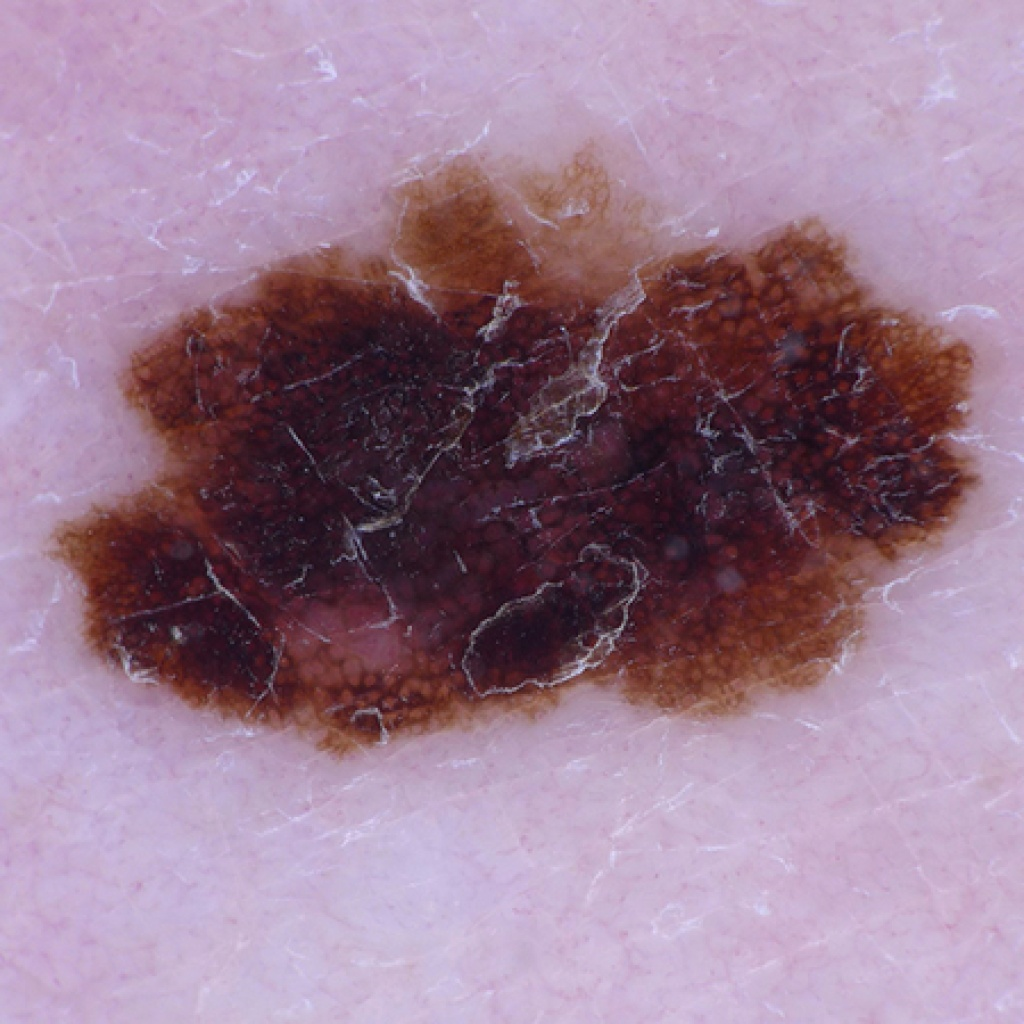
\includegraphics[width=4cm]{../img/bab2/mel.jpg}
            \caption{Kanker kulit MEL} 
            \label{fig:mel}
            Sumber: \citep{Codella2018,Combalia2019,Tschandl2018}
        \end{center} 
    \end{figure}

    \subsection{\textit{Actinic Keratosis} (AK)}
    AK merupakan kanker kulit yang sangat umum diderita. Paparan sinar UV yang sangat tinggi pada tubuh dapat menyebabkan kemunculan AK, seperti pada bagian wajah, kulit kepala, leher, punggung tangan, dan lengan. AK memiliki kemungkinan berevolusi menjadi SCC, akan tetapi tidak memungkinkan untuk memprediksi setiap lesi. Oleh karena itu, pengobatan AK sangat penting untuk menghindari perubahannya menjadi SCC. Seseorang yang berusia lebih dari 40 tahun memiliki kecenderungan untuk terkena AK daripada seseorang yang lebih muda \citep{Dianzani2020}. Kanker kulit \textit{actinic keratosis} seperti terlihat pada Gambar \ref{fig:ak}.
    \begin{figure}[H] 
        \begin{center} 
            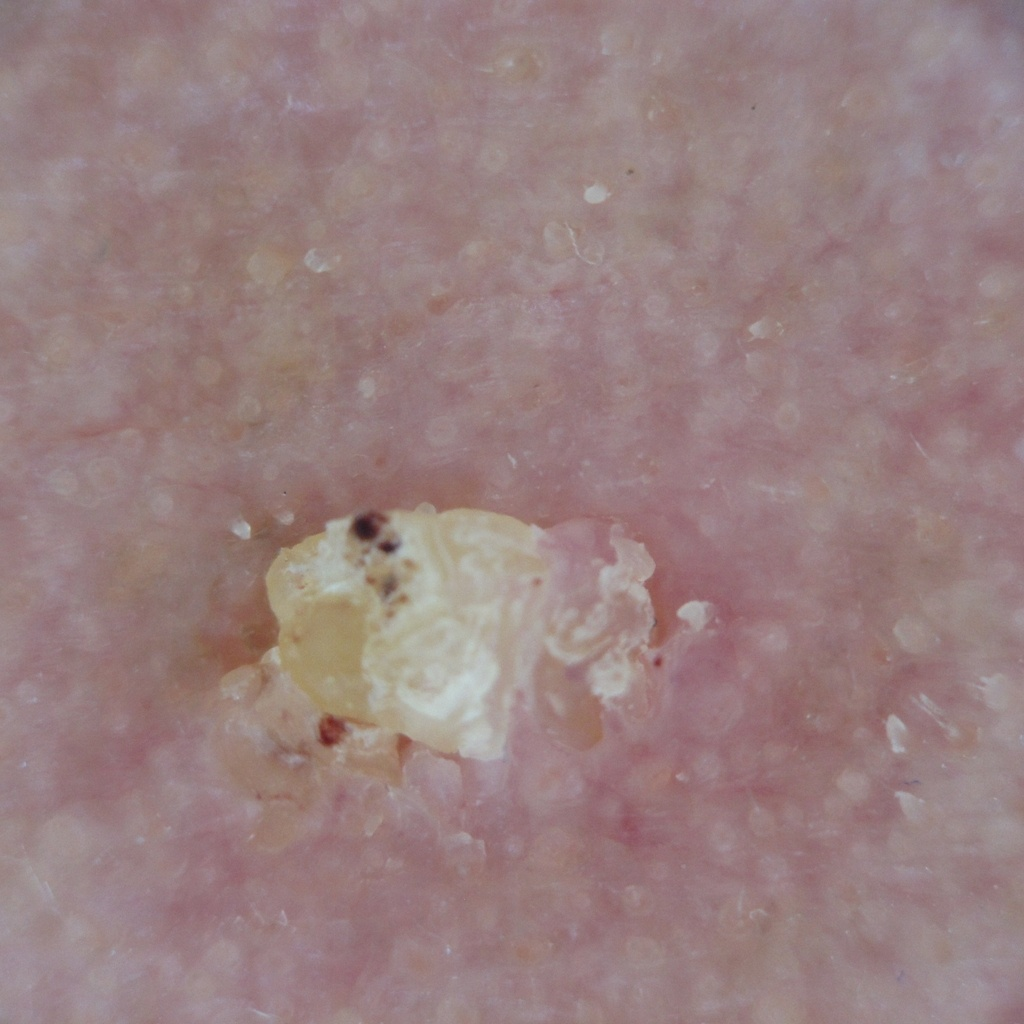
\includegraphics[width=4cm]{../img/bab2/ak.jpg}
            \caption{Kanker kulit AK} 
            \label{fig:ak}
            Sumber: \citep{Codella2018,Combalia2019,Tschandl2018}
        \end{center} 
    \end{figure}

    \subsection{\textit{Melanocytic Nevus} (NV)}
    NV merupakan \textit{benign} yang berasal dari melanosit, pigmen yang dihasilkan sel dendritik, dan biasanya berada pada lapisan basal epidermis di antara keratinosit. NV yang bertumbuh sangat berbahaya karena berpotensi menjadi \textit{melanoma}. NV memiliki ciri-ciri seperti tahi lalat. Jika NV sering terpapar polusi, sinar UV, dan bahan kimia berbahaya dapat berpotensi menjadi \textit{melanoma}. Kanker kulit jenis ini memberikan efek bagi seseorang yang terkena komplikasi, seperti gangguan saraf, kejang, pingsan, dan muntah \citep{Fuadah2020a}. Kanker kulit nevus seperti terlihat pada Gambar \ref{fig:nv}.
    \begin{figure}[H] 
        \begin{center} 
            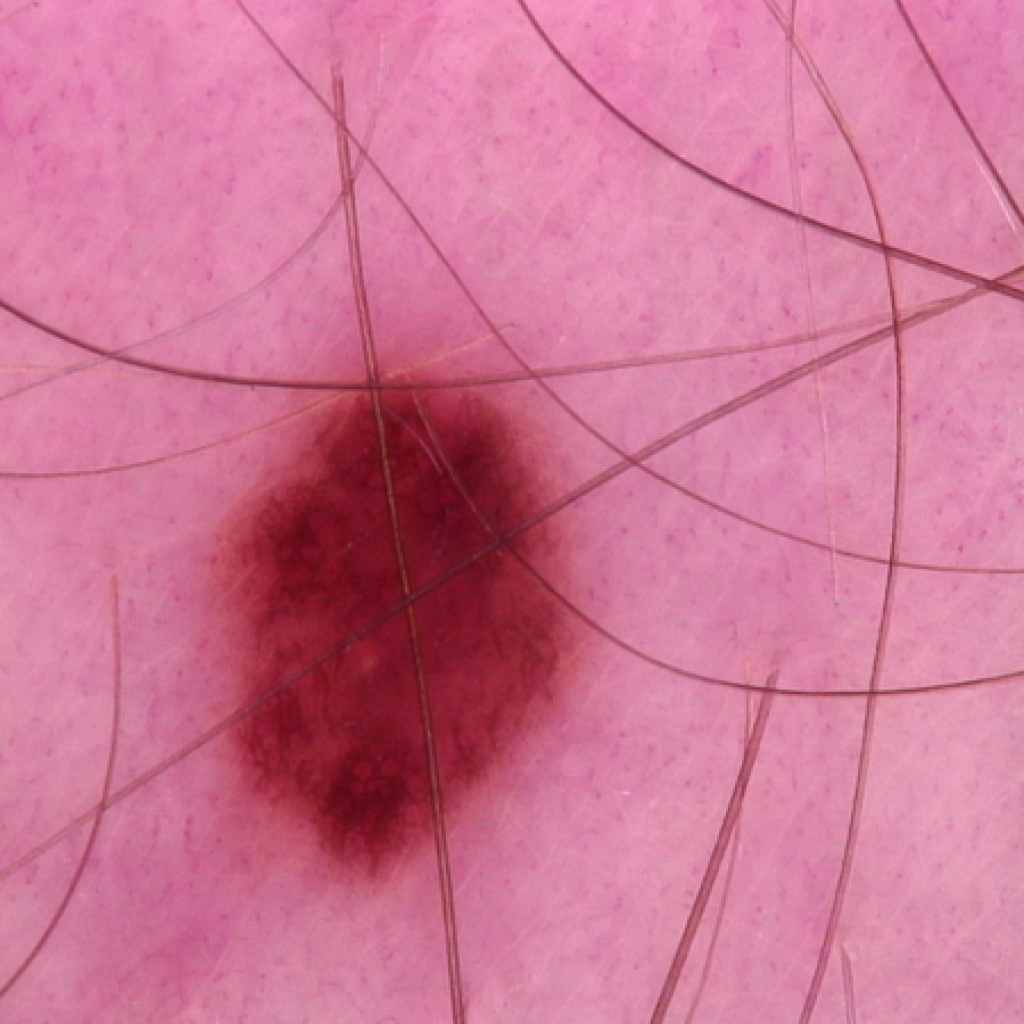
\includegraphics[width=4cm]{../img/bab2/nv.jpg}
            \caption{Kanker kulit NV} 
            \label{fig:nv}
            Sumber: \citep{Codella2018,Combalia2019,Tschandl2018}
        \end{center} 
    \end{figure}

    \subsection{\textit{Basal Cell Carcinoma} (BCC)}
    BCC merupakan kanker kulit yang dari sel-sel basal di dekat persimpangan epidermis-dermis. Kanker kulit jenis ini tumbuh dengan lambat dan tidak bermigrasi. Kemunculan BCC seringkali karena paparan sinar matahari secara langsung dan berlebihan dan biasanya terdapat pada bagian wajah atau leher. Pria dan orang yang semakin tua memiliki presentase lebih tinggi untuk terkena BCC. Diet energi tinggi (khususnya lemak tinggi, vitamin rendah), bahan kimia berbahaya, dan paparan debu juga dapat menyebabkan munculnya BCC. Dalam praktiknya, BCC dibagi menjadi empat jenis, yaitu jenis dangkal, nodular, pigmen, dan titik keras \citep{Sang2019}. Kanker kulit BCC seperti terlihat pada Gambar \ref{fig:bcc}.
    \begin{figure}[H] 
        \begin{center} 
            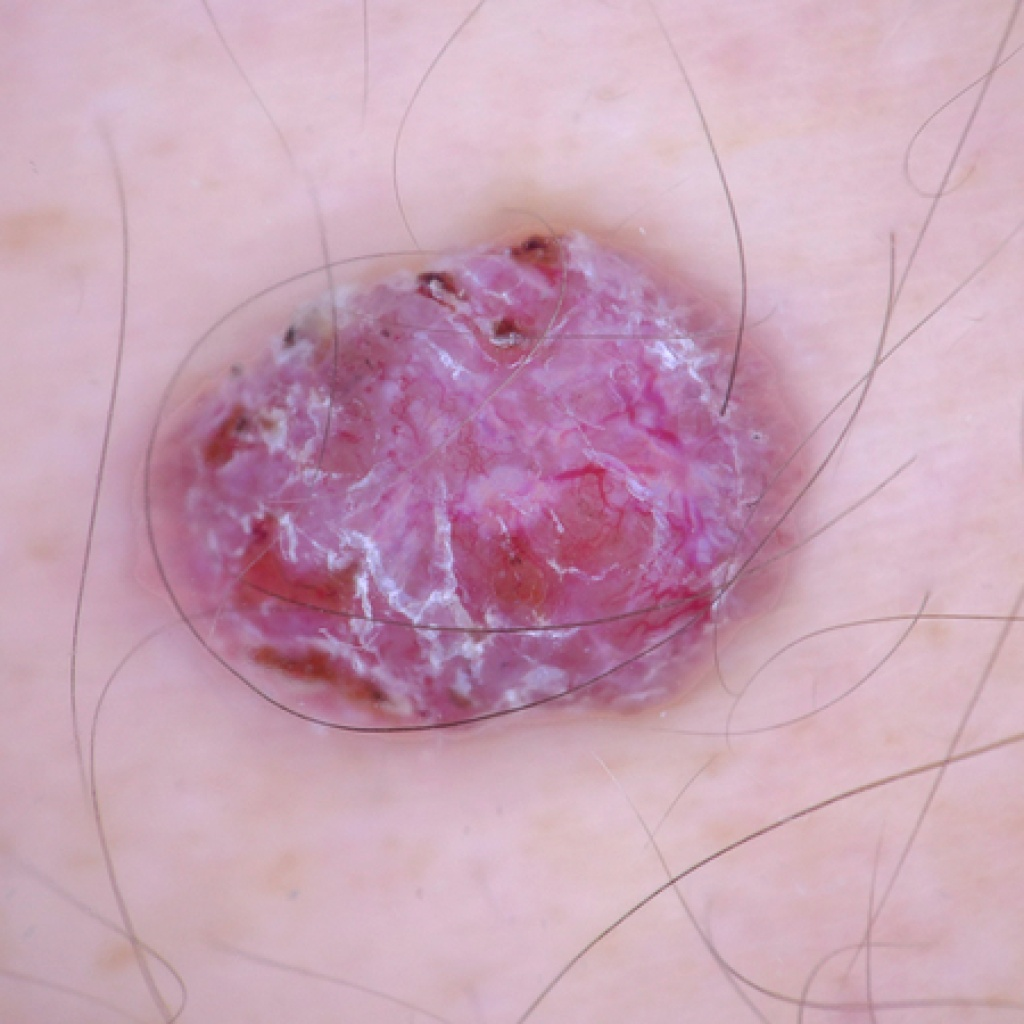
\includegraphics[width=4cm]{../img/bab2/bcc.jpg}
            \caption{Kanker kulit BCC} 
            \label{fig:bcc}
            Sumber: \citep{Codella2018,Combalia2019,Tschandl2018}
        \end{center} 
    \end{figure}

    \subsection{\textit{Squamous Cell Carcinoma} (SCC)}
    SCC merupakan tipe kanker kulit yang tidak agresif. Kanker kulit jenis ini tumbuh dengan lambat. Terapi tanpa pembedahan dapat menangani SCC jika didiagnosis lebih awal. Karena \textit{benign} dapat bertumbuh dengan terus menerus serta menyebar ke tulang, jaringan, dan bahkan kelenjar getah bening jika tidak ditangani sejak awal \citep{Fuadah2020a}. SCC lebih banyak ditemukan pada pria dan usia di atas 60 tahun. Daerah invasi SCC dapat dibagi menjadi tiga bagian, yaitu dangkal, dalam, dan tipe transfer \citep{Sang2019}. Kanker kulit SCC seperti terlihat pada Gambar \ref{fig:scc}.
    \begin{figure}[H] 
        \begin{center} 
            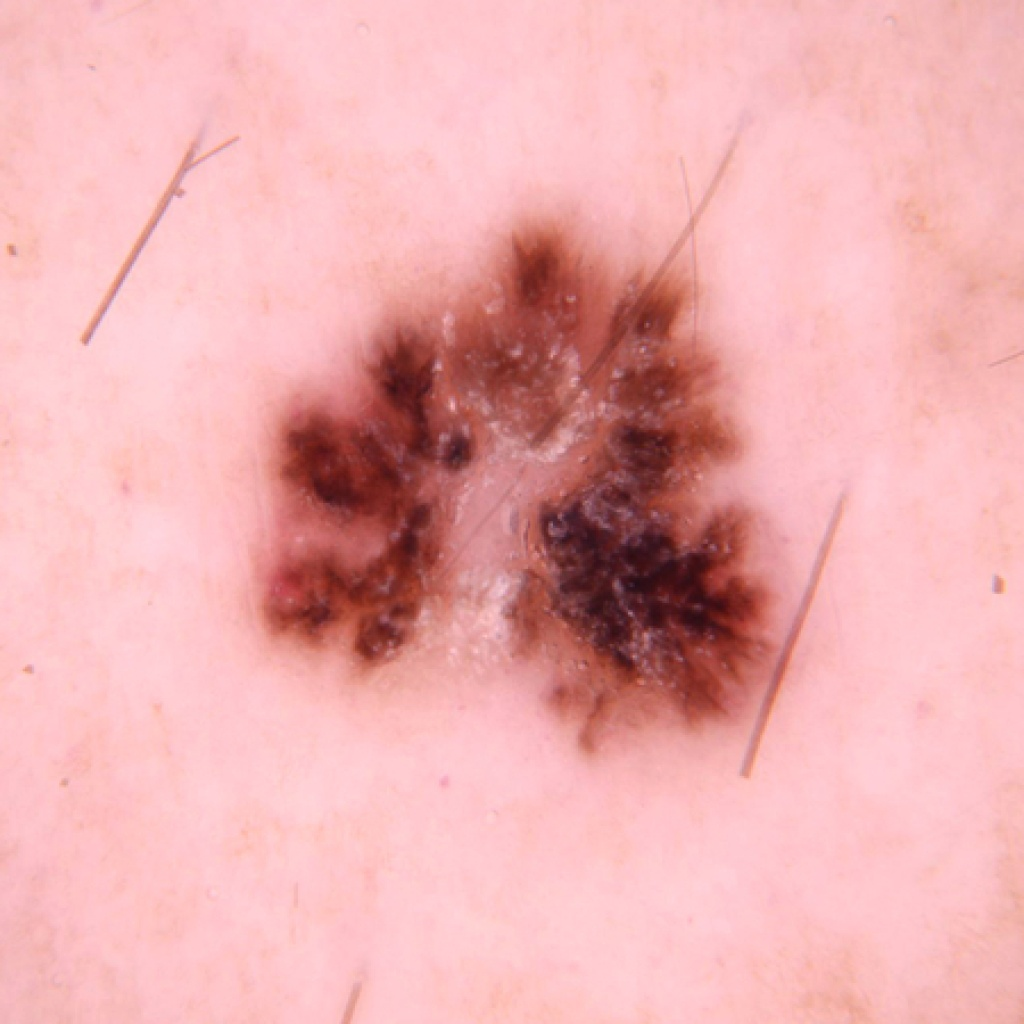
\includegraphics[width=4cm]{../img/bab2/scc.jpg}
            \caption{Kanker kulit SCC} 
            \label{fig:scc}
            Sumber: \citep{Codella2018,Combalia2019,Tschandl2018}
        \end{center} 
    \end{figure}

    \subsection{\textit{Dermatofibroma} (DF)}
    DF termasuk ke dalam kategori \textit{benign}. Kanker kulit jenis ini muncul karena pertumbuhan campuran dari jenis sel di lapisan dermis kulit secara berlebih. Gejala defmatofibroma muncul setelah mengalami beberapa trauma kulit ringan, seperti luka tusuk. Dermatofibroma berukuran sekitar 2-3 mm, berwarna coklat keunguan, berstruktur keras, dan menimbulkan rasa nyeri ketika ditekan \citep{Fuadah2020a}. Kanker kulit DF seperti terlihat pada Gambar \ref{fig:df}.
    \begin{figure}[H] 
        \begin{center} 
            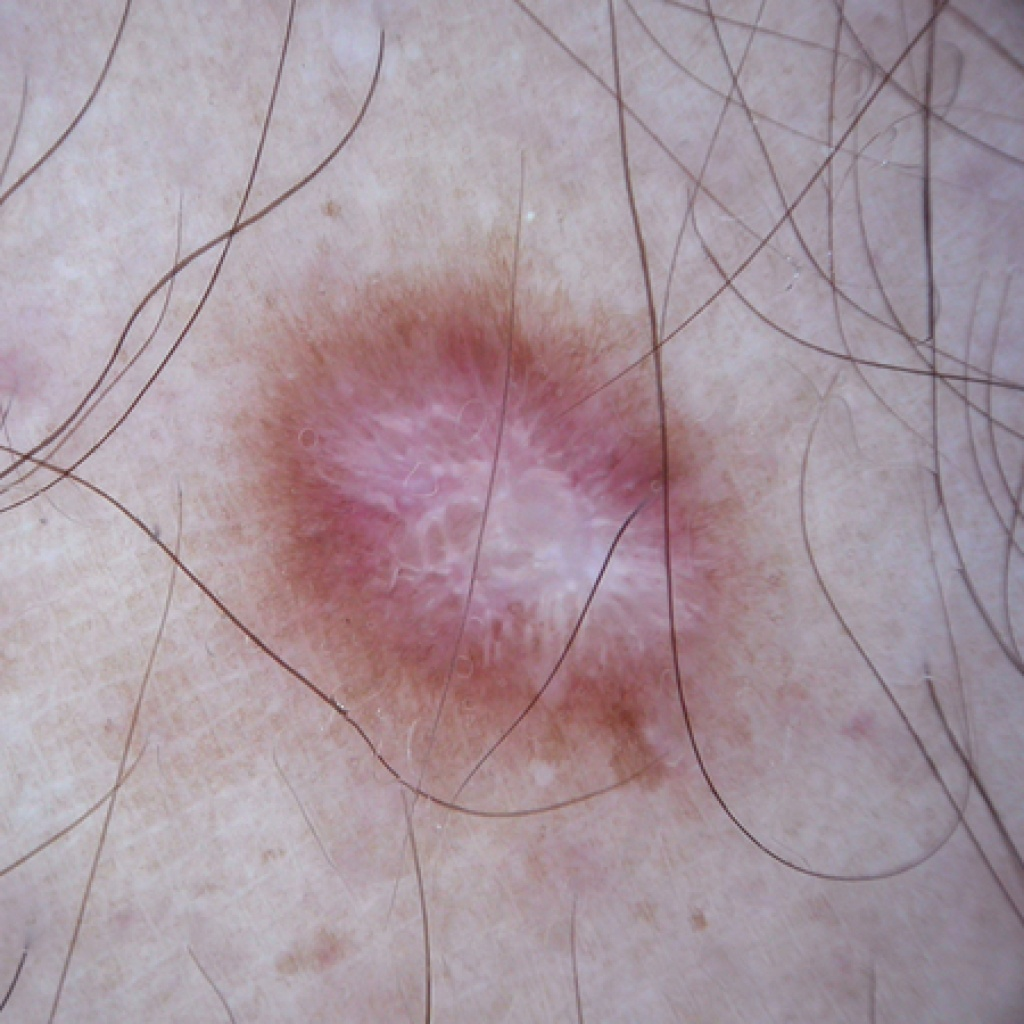
\includegraphics[width=4cm]{../img/bab2/df.jpg}
            \caption{Kanker kulit DF} 
            \label{fig:df}
            Sumber: \citep{Codella2018,Combalia2019,Tschandl2018}
        \end{center} 
    \end{figure}

    \subsection{\textit{Benign Keratosis Lesion} (BKL)}
    BKL merupakan kanker kulit yang tidak berbahaya dan tumbuh dengan warna coklat, hitam, atau coklat lilin. BKL cenderung tidak berbahaya dan tidak memerlukan perawatan khusus. Tampilan umum dari BKL berupa bercak bulat atau oval yang seakan-akan menempel pada kulit. BKL lebih sering terjadi seiring bertambahnya usia seseorang. Tempat tumbuhnya BKL pada kulit yang mengandung rambut dan mukosa. BKL juga ditemukan di daerah genital pria \citep{Hall2019}. Kanker kulit BKL seperti terlihat pada Gambar \ref{fig:bkl}.
    \begin{figure}[H] 
        \begin{center} 
            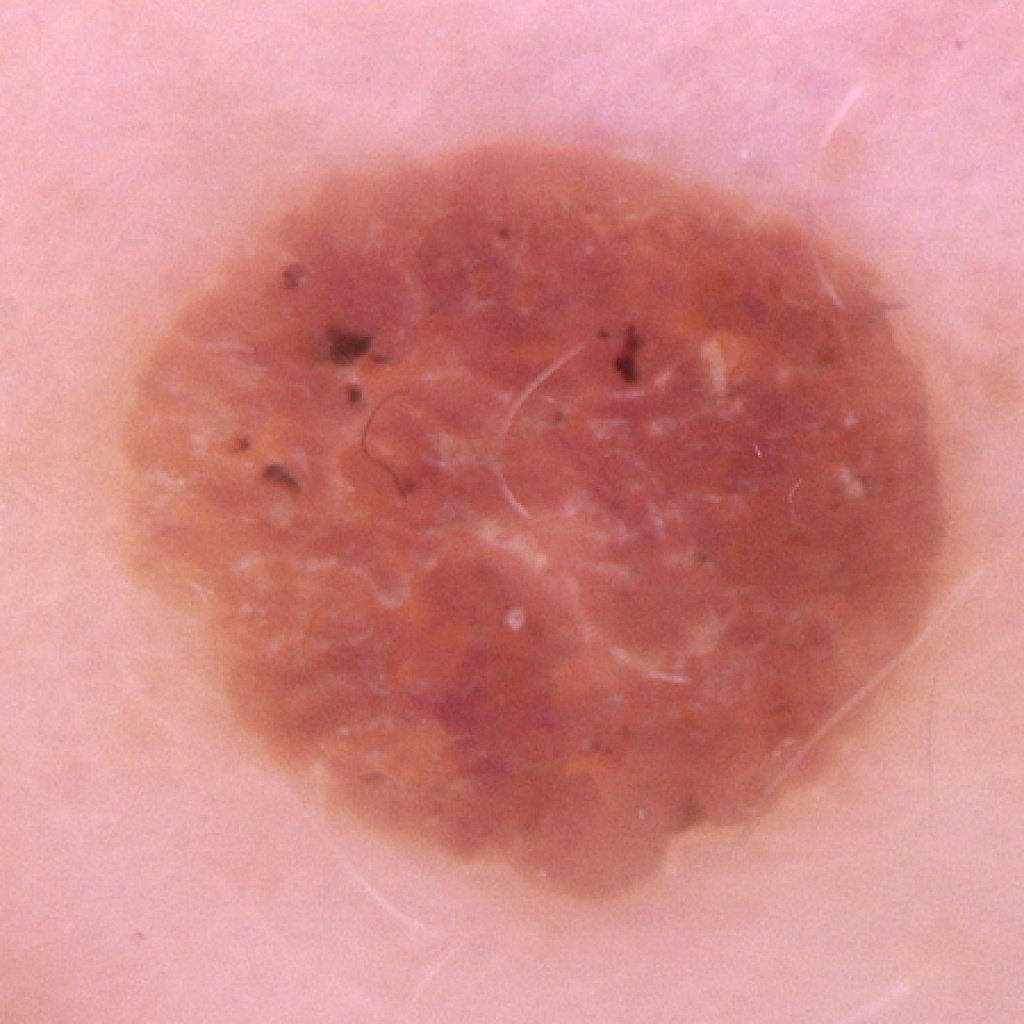
\includegraphics[width=4cm]{../img/bab2/bkl.jpg}
            \caption{Kanker kulit BKL} 
            \label{fig:bkl}
            Sumber: \citep{Codella2018,Combalia2019,Tschandl2018}
        \end{center} 
    \end{figure}

    \subsection{\textit{Vascular Lesion} (VASC)}
    VASC atau biasa disebut sebagai tanda lahir merupakan kanker yang ada pada kulit dan jaringan di bawahnya \citep{Balas2018}. Kanker kulit jenis ini relatif umum terjadi. Terdapat tiga kategori utama dari VASC, yaitu \textit{Hemangioma}, \textit{Malformasi Vaskular}, dan \textit{Granuloma Piogenik}. Ketiga jenis tanda lahir ini terlihat serupa, meskipun ketiganya memiliki perawatan yang berbeda-beda. \textit{Hemangioma} merupakan jenis kanker kulit yang umum pada anak-anak. \textit{Hemangioma} dapat dipantau oleh dokter kulit atau dokter anak karena kanker kulit jenis ini tumbuh secara alami dan tanpa perawatan. Meskipun tidak banyak \textit{Hemangioma} yang perlu perawatan khusus karena berada pada daerah yang tidak tepat. \textit{Malformasi vaskular} merupakan kesalahan kongenital dalam pembentukan pembuluh darah. \textit{Malformasi vaskular} memerlukan perawatan khusus karena terkait dengan kesalahan fungsi pada pembuluh darah. \textit{Granuloma piogenik} merupakan kanker kulit tidak berbahaya yang terbentuk sebagai respon terhadap cedera jaringan lokal. Kanker kulit jenis ini umumnya muncul pada anak-anak dan ibu hamil pada daerah mulut dan ujung jari \citep{Rastogi2020}. Kanker kulit VASC seperti terlihat pada Gambar \ref{fig:vasc}.
    \begin{figure}[H] 
        \begin{center} 
            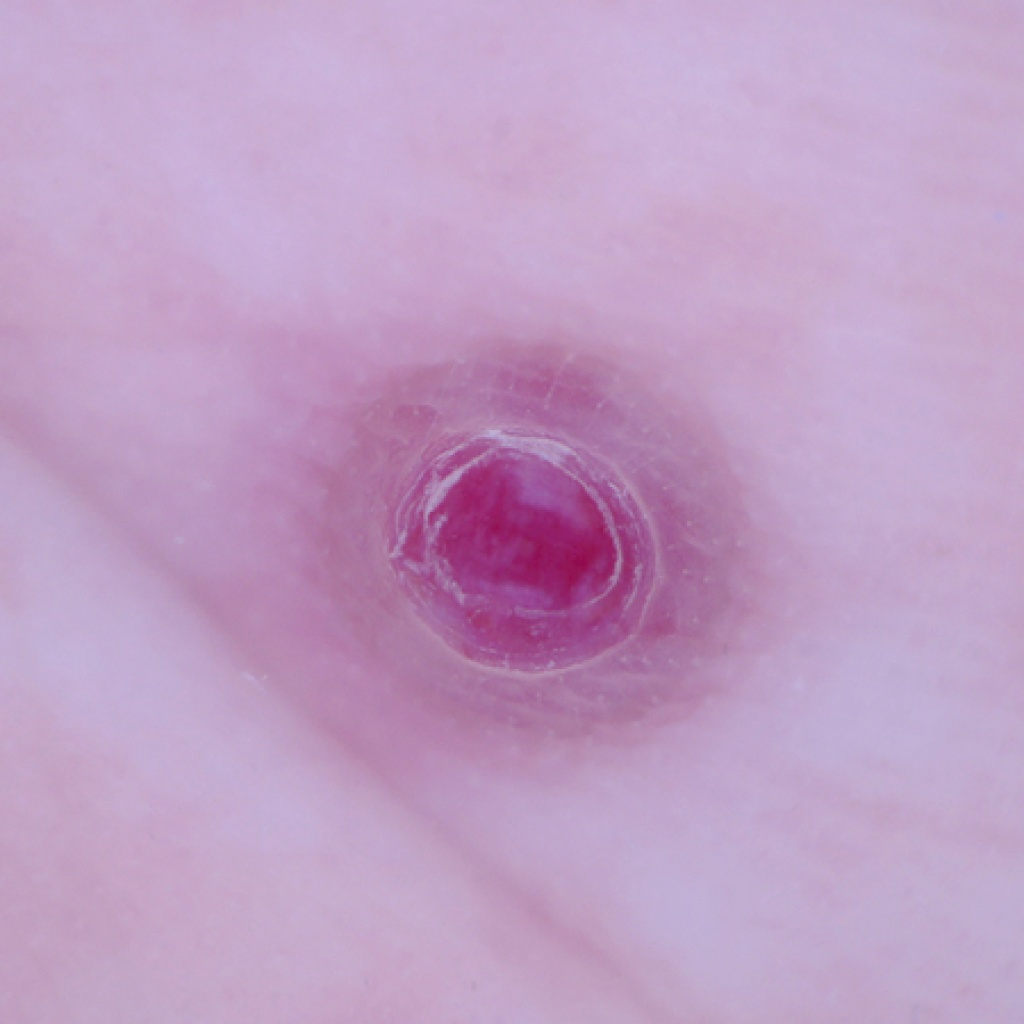
\includegraphics[width=4cm]{../img/bab2/vasc.jpg}
            \caption{Kanker kulit VASC} 
            \label{fig:vasc}
            Sumber: \citep{Codella2018,Combalia2019,Tschandl2018}
        \end{center} 
    \end{figure}

\section{Citra Digital}
Sebagian besar informasi didapatkan dalam bentuk gelombak elektrik dan sinyal. Citra merupakan informasi yang dapat diubah ke dalam bentuk sinyal dua dimensi. Fungsi intensitas cahaya dalam bentuk diskrit pada ruang dua dimensi disebut citra digital. Pada citra digital terdapat beberapa elemen baris dan kolom yang disebut piksel. Piksel pada citra memiliki atribut amplitudo $f(a,b)$ dan koordinat $(x,y)$. Amplitudo $f(a,b)$ menunjukkan intensitas warna yang ada pada citra. Koordinat $(x,y)$ merepresentasikan letak piksel dalam sebuah citra digital \citep{Ratna2020}. Sebuah citra digital dapat dilihat sebagai gambaran visual dari matriks yang berisi bilangan bulat (\textit{integer}). Bilangan bulat tersebut menunjukkan derajat keabuan untuk citra \textit{grayscale} dan menunjukkan derajat warna untuk citra RGB \citep{Blackledge2005,Septiaji2018}.

Fungsi dari dua variabel $f(x,y)$ merepresentasikan citra berdasarkan derajat keabuan $(x,y)$ sehingga citra tersebut dapat diubah menjadi fungsi diskrit sebagai citra digital seperti terlihat pada Persamaan (\ref{eq:citra}).

\begin{align}
    f_{ij} \textnormal{ dimana } f_{ij} &\equiv f(x_i, y_i)
    \label{eq:citra}
\end{align}

$f_{ij}$ merupakan nilai fungsi pada $x=x_i$ dan $y=y_i$ sehingga bisa didefinisikan sebagai matriks seperti pada Persamaan \ref{eq:citra2}.

\begin{align}
    f_{ij} &=
    \begin{bmatrix}
        f_{11} &f_{12} &\cdots &f_{1n}\\
        f_{21} &f_{22} &\cdots &f_{2n}\\
        \vdots &\vdots &\ddots &\vdots\\
        f_{n1} &f_{n2} &\cdots &f_{nn}\\
    \end{bmatrix}
    \label{eq:citra2}
\end{align}

    \subsection{Citra RGB}
    Citra digital yang memiliki tiga kanal warna merupakan citra RGB. Tiga kanal warna tersebut adalah \textit{Red}, \textit{Green}, \textit{Blue} (RGB). Setiap lapisan warna memiliki nilai piksel antara $0$ sampai $255$. Pada umumnya, nilai piksel ini tersimpan pada memori komputer atau berkas tertentu dalam bentuk 8-bit atau $2^8$ warna \citep{Septiaji2018}. Citra RGB seperti terlihat pada Gambar \ref{fig:color}.

    \begin{figure}[H]
        \begin{center}
            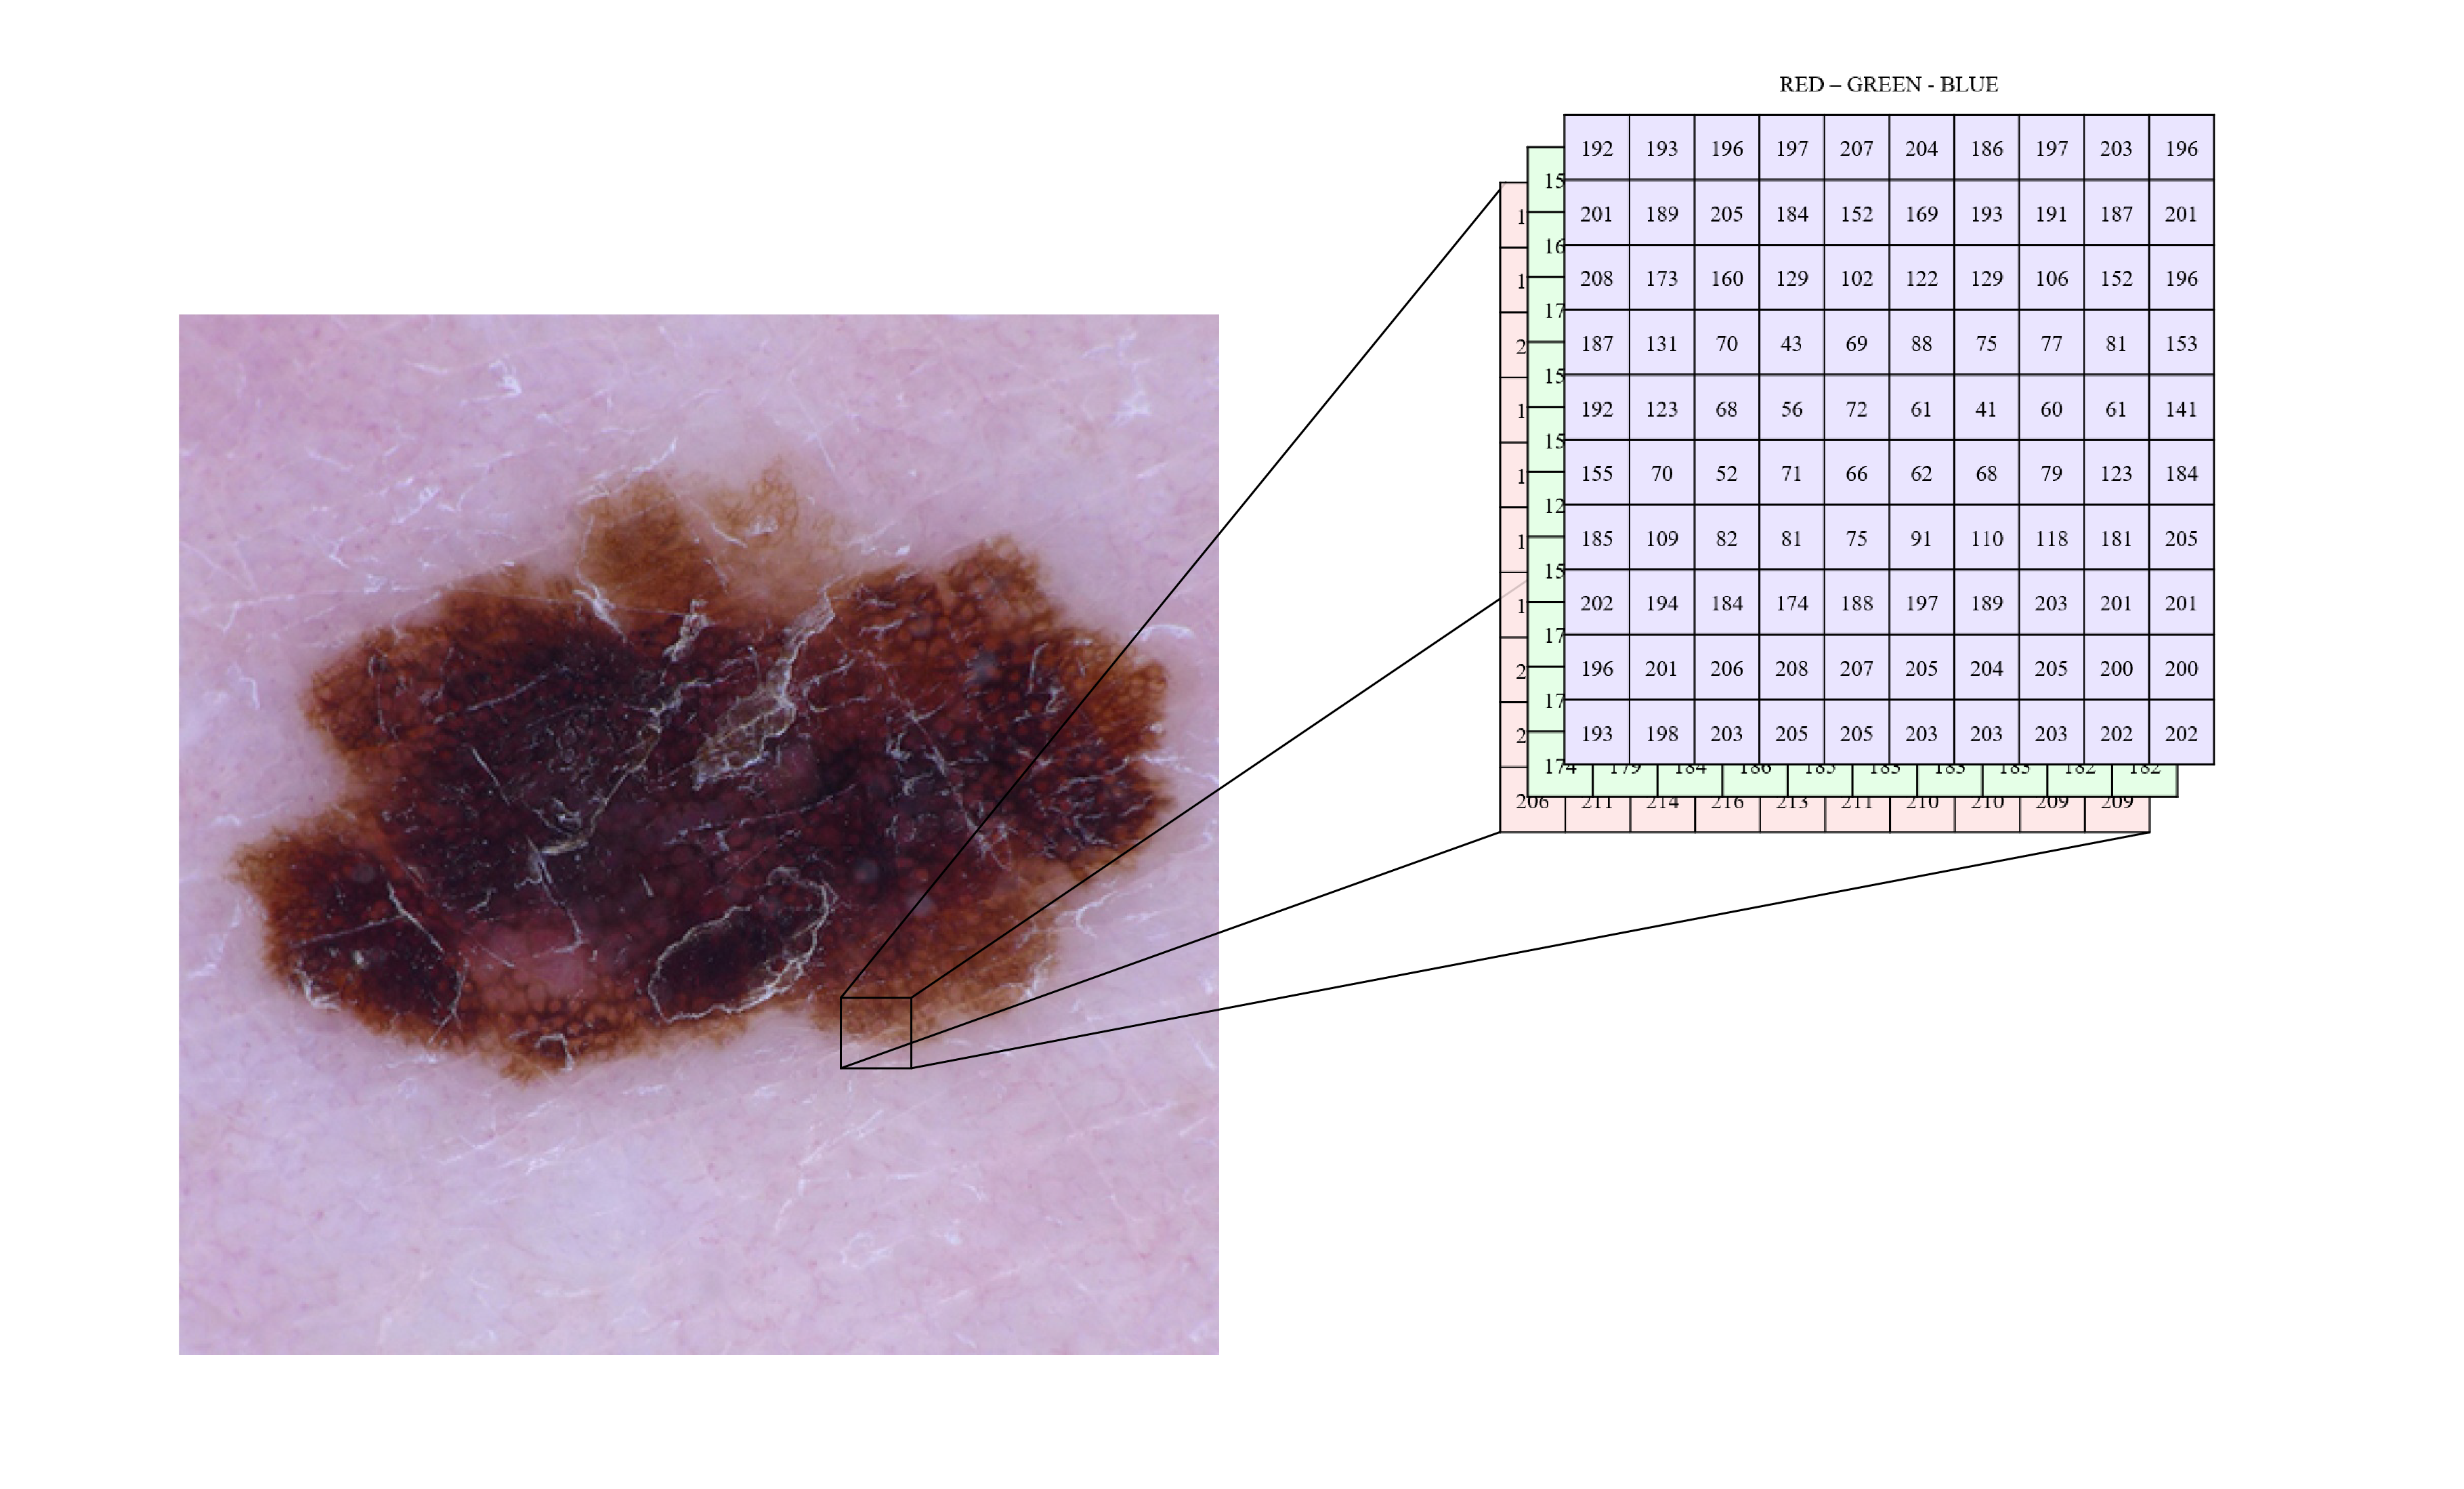
\includegraphics[width=8cm]{../img/bab2/warna.png}
            \caption{Citra warna beserta nilai pikselnya}
            \label{fig:color}
            Sumber: \citep{Kusumanto2011}
        \end{center}
    \end{figure}

    \subsection{Citra \textit{Grayscale}}
    Citra \textit{grayscale} hanya memiliki satu kanal warna yang menunjukkan intensitas derajat keabuan. Pada umumnya, nilai piksel yang dimiliki citra \textit{grayscale} berkisar antara $0$ sampai $255$ \citep{Kusumanto2011}. Citra \textit{grayscale} seperti terlihat pada Gambar \ref{fig:grayscale}.

    \begin{figure}[H]
        \begin{center}
            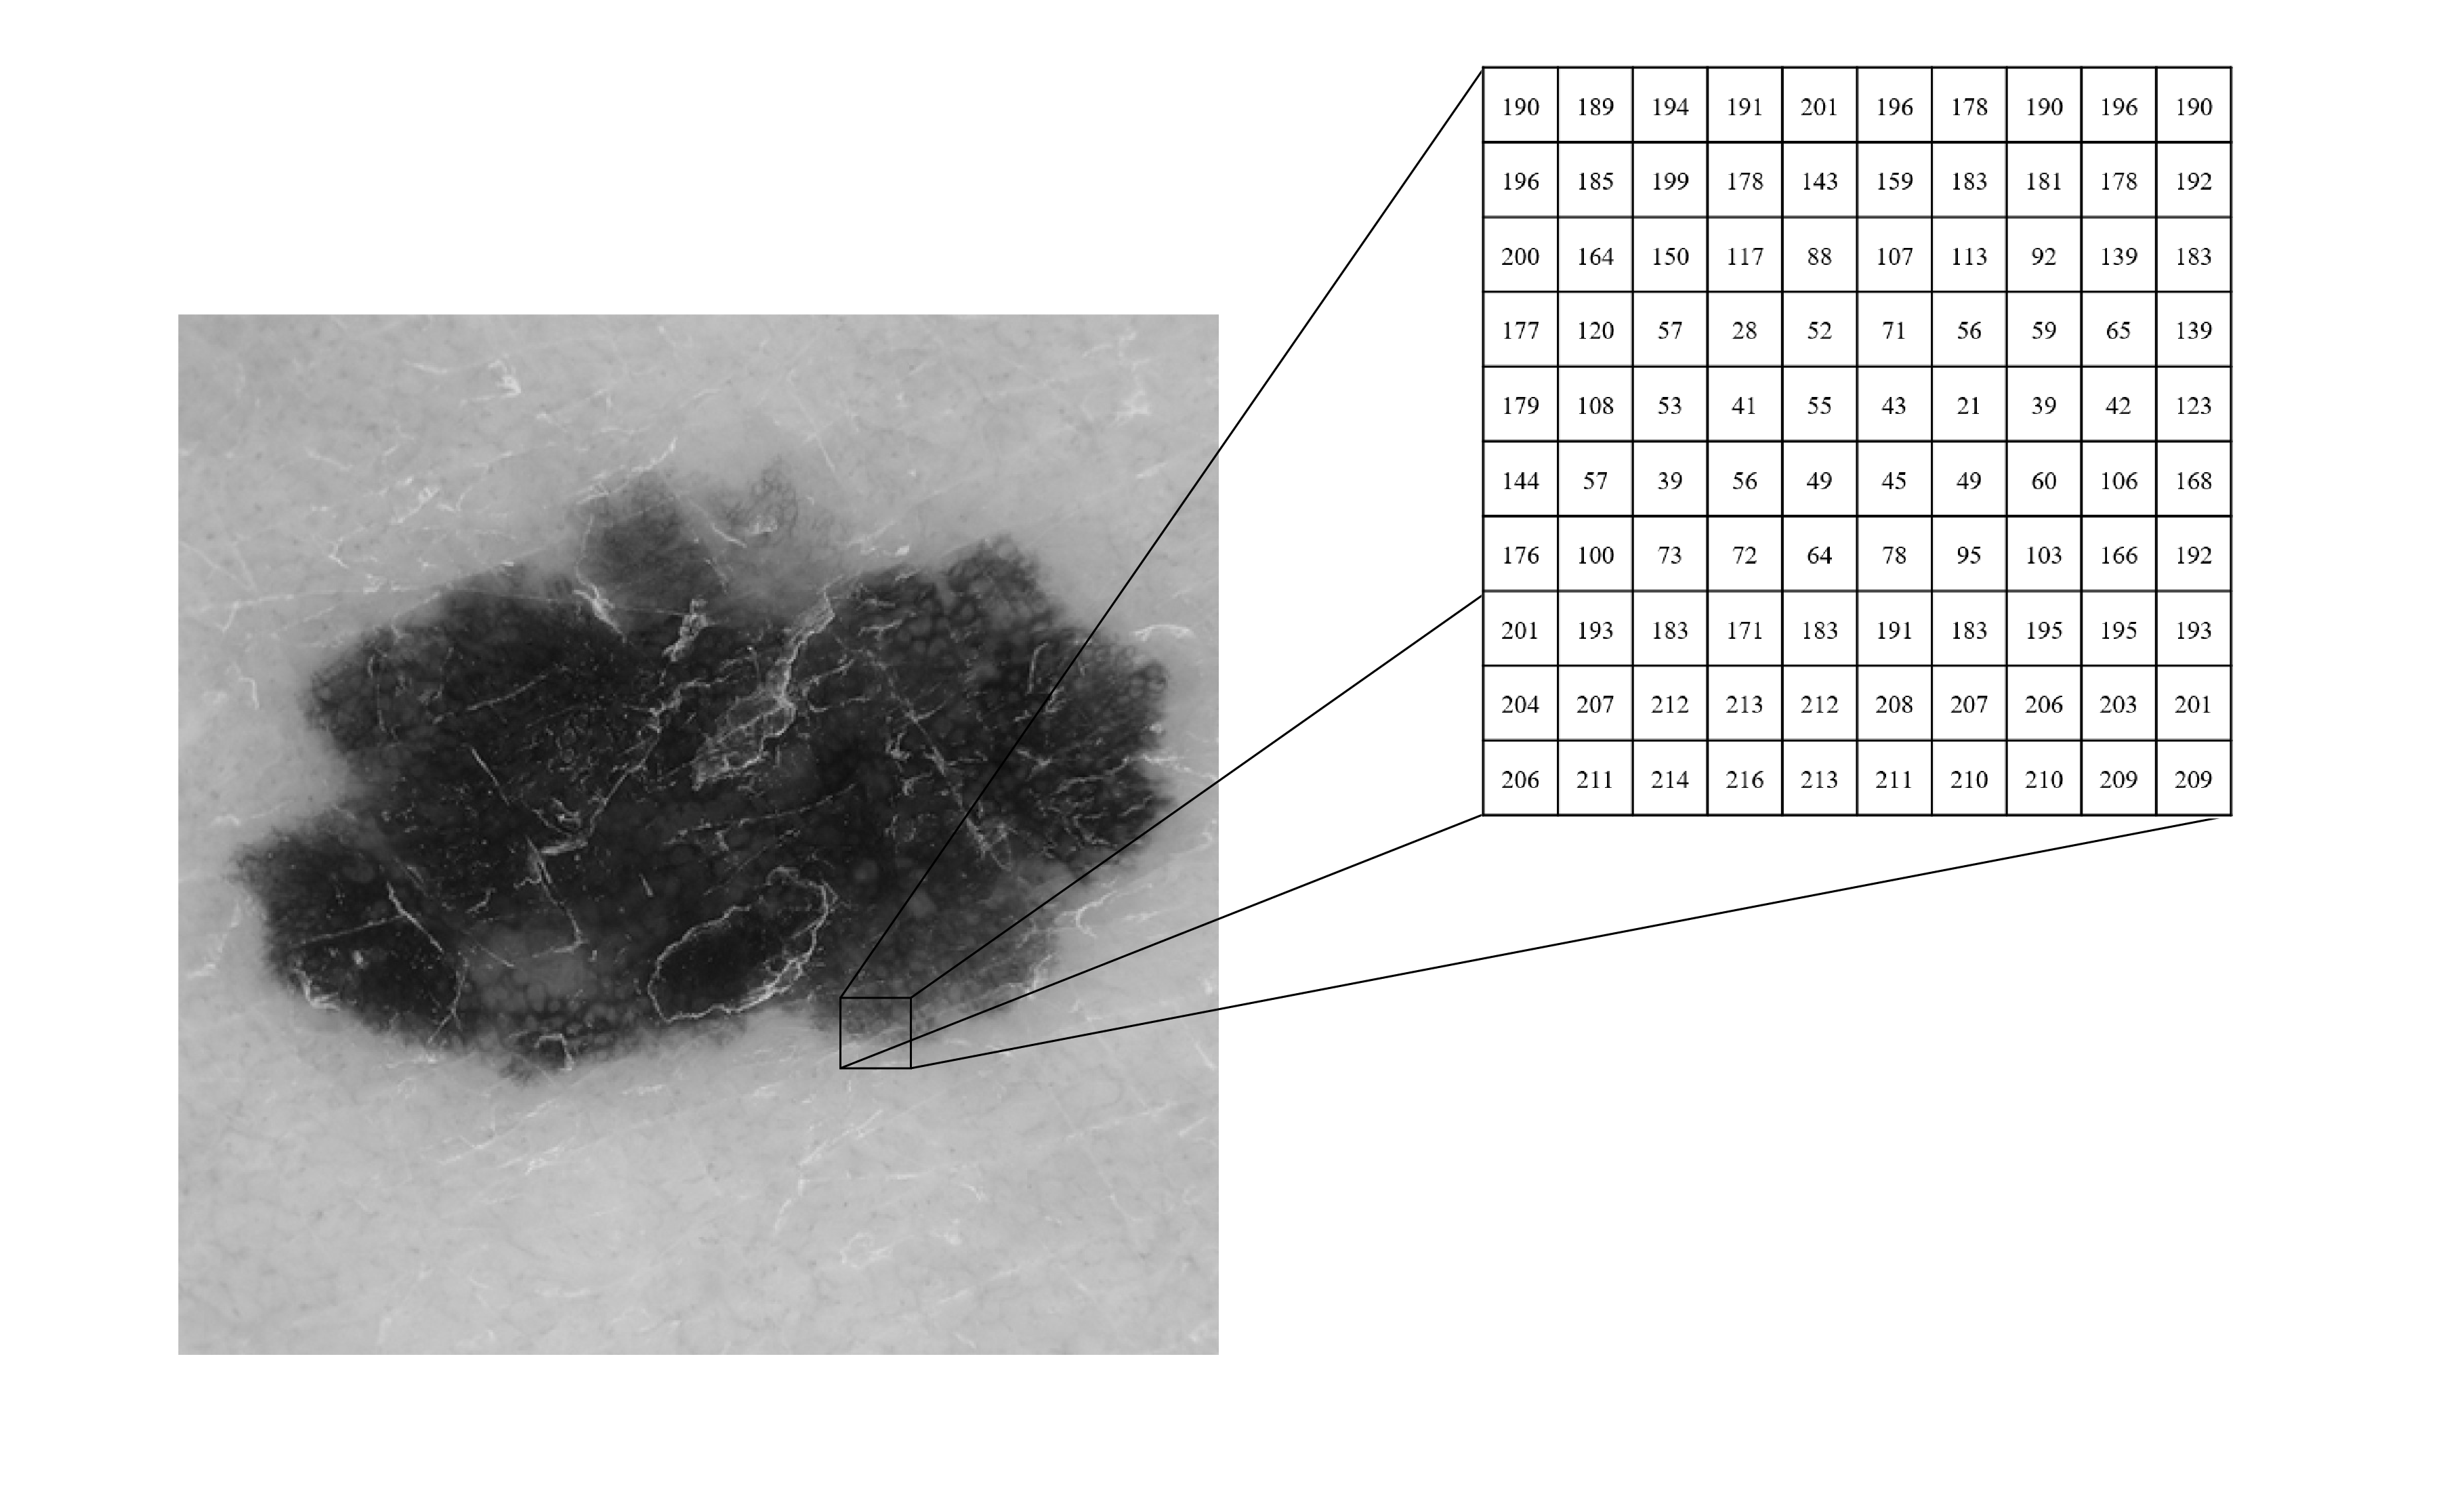
\includegraphics[width=8cm]{../img/bab2/grayscale.png}
            \caption{Citra \textit{grayscale} beserta nilai pikselnya}
            \label{fig:grayscale}
            Sumber: \citep{Kusumanto2011}
        \end{center}
    \end{figure}

    \subsection{Citra \textit{Binary}}
    Citra \textit{binary} hanya memiliki dua nilai, yaitu $0$ atau $1$. Citra ini termasuk citra yang paling sederhana karena nilai $0$ pada suatu piksel citra \textit{binary} menggambarkan warna hitam sedangkan nilai $1$ menggambarkan warna putih \citep{Kusumanto2011}. Contoh citra \textit{binary} seperti terlihat pada Gambar \ref{fig:binary}.

    \begin{figure}[H]
        \begin{center}
            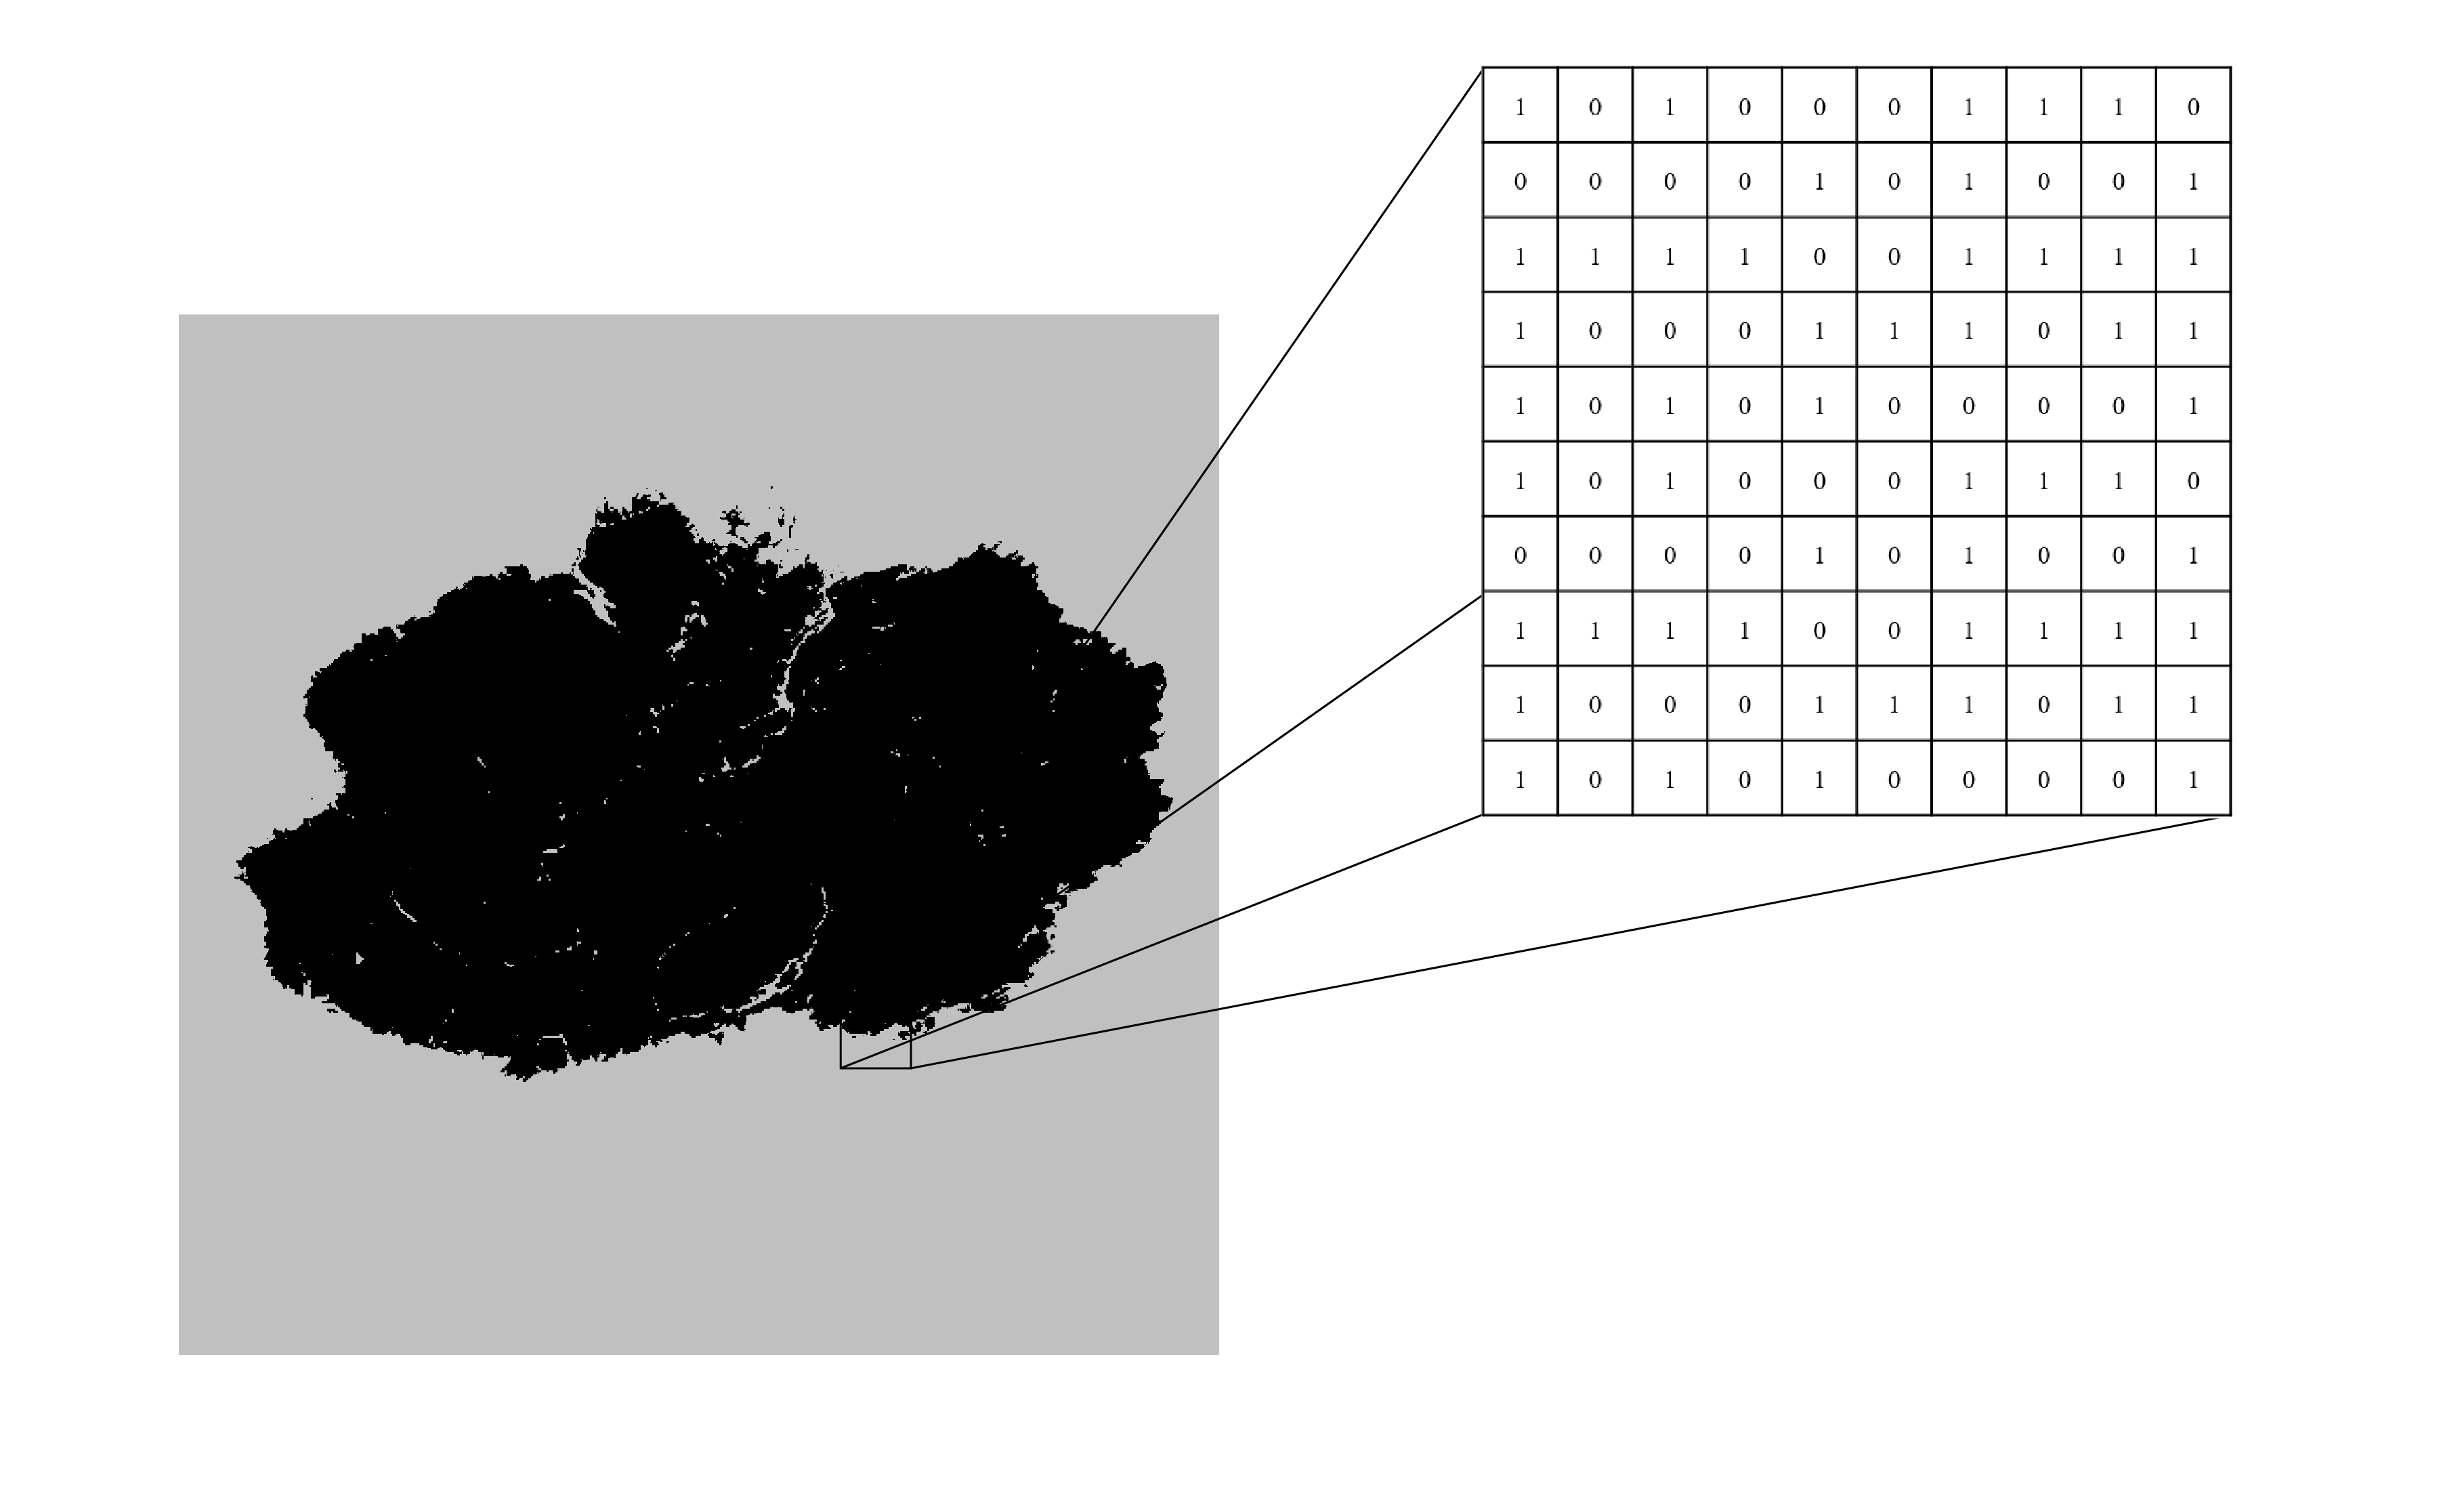
\includegraphics[width=8cm]{../img/bab2/biner.png}
            \caption{Citra \textit{binary} beserta nilai pikselnya}
            \label{fig:binary}
            Sumber: \citep{Kusumanto2011}
        \end{center}
    \end{figure}

    % TODO: kurang jelas
    \subsection{Citra Dermoskopi}
    Dermoskopi menuju pada istilah dalam pemeriksaan kulit menggunakan mikroskop. Teknik ini merupakan teknik pencitraan kulit beresolusi tinggi yang memungkinkan visualisasi struktur kulit tanpa terhalang oleh pantulan permukaan kulit. Hal ini bertujuan untuk mengamati kulit dengan lebih detil dan mempermudah diagnosis kanker kulit. Sehingga, hasil dari teknik pencitraan kulit menggunakan mikroskop ini disebut sebagai citra dermoskopi \citep{Celebi2019}. Contoh citra dermoskopi seperti terlihat pada Gambar \ref{fig:dermoscopy}.

    \begin{figure}[H]
        \begin{center}
            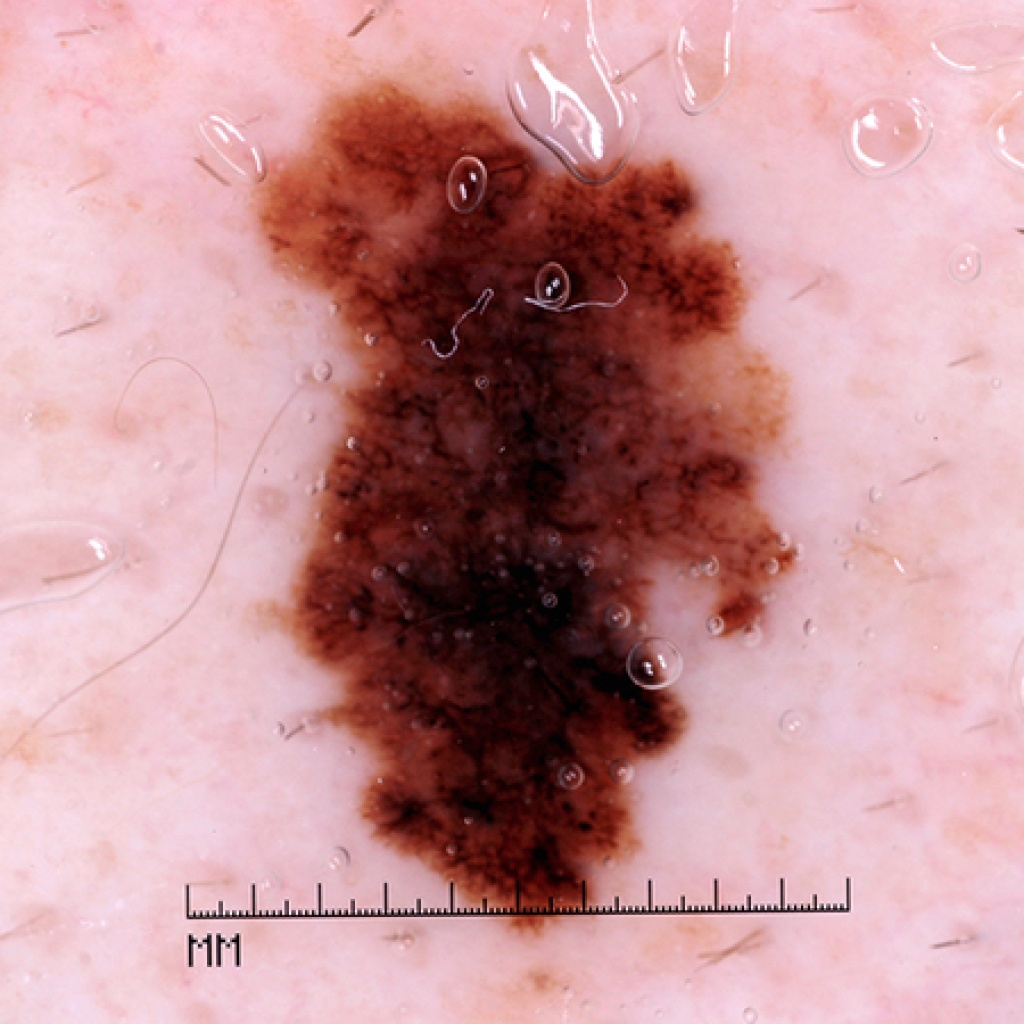
\includegraphics[width=4cm]{../img/bab2/dermoscopy.jpg}
            \caption{Citra \textit{dermoscopy} yang mengandung kanker kulit \textit{melanoma}}
            \label{fig:dermoscopy}
            Sumber: \citep{Nersisson2021a}
        \end{center}
    \end{figure}

\section{\textit{Resize}}
\textit{Resize} atau penskalaan citra merupakan proses rekontruksi citra untuk mengubah ukuran sebuah citra \citep{Morsy2018}. Pengubahan ukuran citra biasanya terjadi untuk menyesuaikan ukuran citra dan mengurangi waktu komputasi \citep{AhmedThaajwer2020a,Umamaheswari2018}. Penelitian ini menggunakan Interpolasi Bilinier untuk melakukan \textit{resize}. Perhitungan untuk melakukan \textit{resize} seperti terlihat pada Persamaan \ref{eq:resize} dimana $w_x = \frac{x-x_1}{x_2-x_1}$ dan $w_y = \frac{y-y_1}{y_2-y_1}$. Pada Persamaan \ref{eq:resize} $x$ merupakan lebar, $y$ merupakan tinggi, $(y_1, x_1)$, $(y_1, x_2)$, $(y_2, x_1)$, $(y_2, x_2)$ merupakan koordinat nilai piksel, $A$, $B$, $C$, $D$ merupakan nilai piksel, dan $Z$ merupakan nilai interpolasi antara dua nilai interpolasi $X$ dan $Y$ \citep{Gribbon2004}. Contoh penskalaan citra seperti terlihat pada Gambar \ref{fig:resize}.

\begin{align}
    X &= A(1-w_x)+Bw_x\nonumber\\
    Y &= C(1-w_x)+Dw_x\nonumber\\
    Z &= X(1-w_y)+Yw_y\nonumber\\
    \label{eq:resize}
    &= A(1-w_x)(1-w_y) + Bw_x(1-w_y) + C(1-w_x)w_y + Dw_{x}w_{y}
\end{align}

\begin{figure}[H]
    \centering
    \begin{tabular}{cc}
        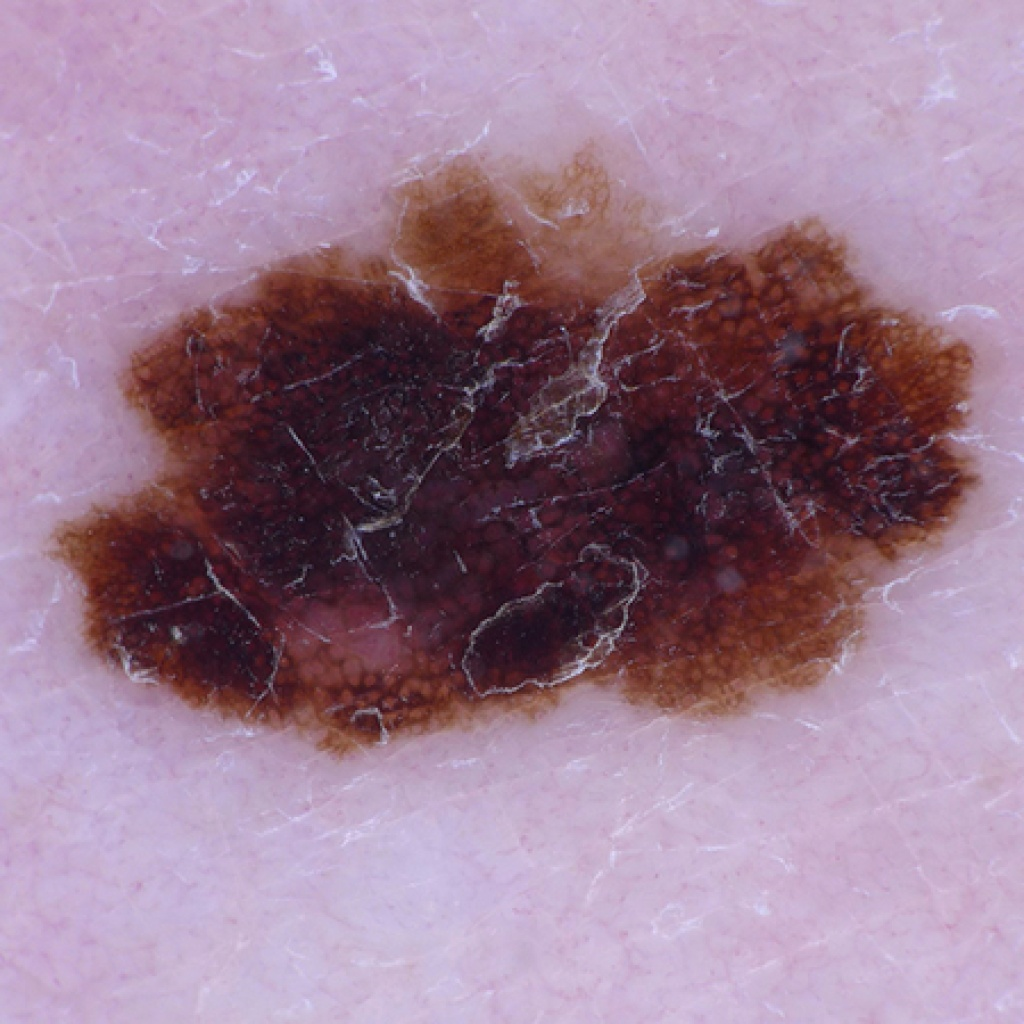
\includegraphics[width=4cm]{../img/bab2/mel.jpg}
        &
        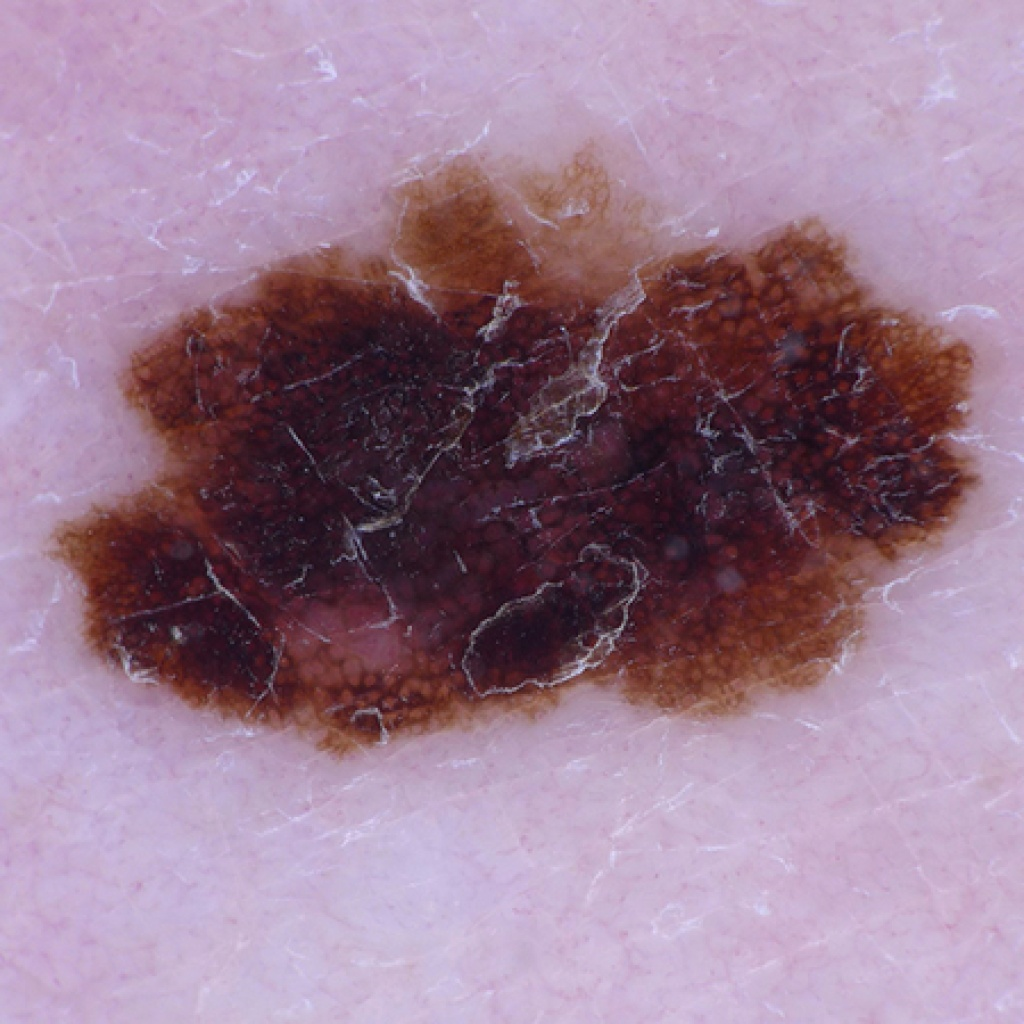
\includegraphics[width=2cm]{../img/bab2/mel.jpg}\\
        (a) &(b)\\
    \end{tabular}
    \caption{(a) Citra sebelum diubah berukuran $500\times 500$ piksel (b) Citra setelah diubah berukuran $200\times 200$ piksel}
    \label{fig:resize}
    Sumber: \citep{Morsy2018}
\end{figure}

\section{Deteksi Objek}
Deteksi objek merupakan salah satu proses penting dalam \textit{computer vision} dengan mendeteksi sebuah objek pada sebuah citra dengan kelas tertentu, misalnya mobil, manusia, hewan secara spesifik, atau yang lainnya. Sebagai salah satu bagian penting dalam \textit{computer vision}, deteksi objek merupakan dasar dari beberapa tugas \textit{computer vision} seperti melacak objek, segmentasi objek, dan mengambil teks dalam gambar \citep{Zou2019}. Contoh deteksi objek seperti terlihat pada Gambar \ref{fig:obj-det}.

\begin{figure}[H]
    \begin{center}
        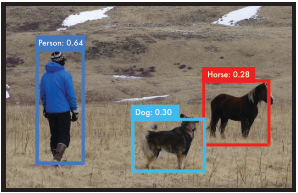
\includegraphics[width=7cm]{../img/bab2/object-detection.PNG}
        \caption{Deteksi objek yang dilakukan oleh model YOLO}
        \label{fig:obj-det}
        Sumber: \citep{Redmon2016a}
    \end{center}
\end{figure}

Pada Gambar \ref{fig:obj-det}, metode YOLO yang dikembangkan oleh Redmon, dkk. dapat melakukan deteksi objek pada citra dengan memberikan \textit{bounding box} pada objek yang telah ditemukan pada citra \citep{Redmon2016a}. Objek manusia, anjing, dan kuda pada Gambar \ref{fig:obj-det} dapat dideteksi oleh YOLO secara bersamaan. Pada setiap deteksi, YOLO mengeluarkan probabilitas kelas beserta \textit{bounding box} objek.

\section{\textit{Convolutional Neural Networks} (CNN)}
CNN termasuk ke dalam \textit{deep learning} dan perkembangan dari \textit{Multi Layer Perceptron} (MLP). CNN merupakan algoritma yang mirip dengan \textit{Artificial Neural Network} (ANN). Bahkan karena kemiripannya, strategi pengembangan ANN dapat diterapkan pada CNN. Data masukan pada CNN berupa matriks dari citra sehingga menghasilkan keluaran berupa skor atau bobot tertentu. Layer terakhir pada sebuah CNN mengandung loss function yang diasosiasikan dengan kelas tertentu. Pada umumnya, perbedaan ANN dan CNN terletak pada CNN yang lebih mengutamakan pengenalan pola pada sebuah citra. Hal ini dapat mengeluarkan fitur spesifik pada sebuah citra sehingga diolah pada arsitektur CNN.

Berdasarkan kemampuan CNN yang dapat mengolah data citra, neuron pada CNN terdiri atas neuron tiga dimensi. Neuron tersebut mengandung dimensi spasial dari data masukan, yaitu \textit{height}, \textit{width}, dan \textit{depth}. \textit{Depth} tidak mengacu pada jumlah layer pada jaringan, akan tetapi mengacu pada dimensi ketiga dari \textit{activation volume}. Neuron pada setiap layer hanya terkoneksi terhadap layer yang mendahuluinya. Arsitektur dasar CNN terdiri dari tiga jenis layer, yaitu \textit{convolutional layer}, \textit{pooling layer}, dan \textit{fully-connected layers}. Arsitektur dasar pada CNN seperti terlihat pada Gambar \ref{fig:cnn}.

\begin{figure}[H]
    \begin{center}
        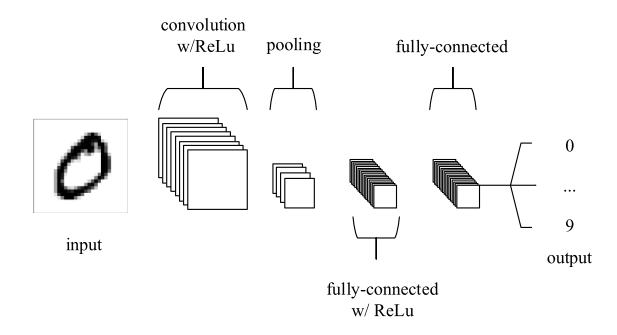
\includegraphics[width=12cm]{../img/bab2/cnn.png}
        \caption{Arsitektur dasar dari CNN}
        \label{fig:cnn}
        Sumber: \citep{OShea2015}
    \end{center}
\end{figure}

    \subsection{\textit{Convolutional Layer}}
    \textit{Convolutional Layer} merupakan layer utama dari CNN karena pada layer ini citra diolah dan dipelajari oleh CNN. \textit{Convolutional layer} menerapkan operasi konvolusi dengan tujuan mendapatkan fitur-fitur yang ada pada citra, seperti \textit{edge}, \textit{color}, \textit{shape}, dan fitur lainnya. Operasi konvolusi terjadi antara matriks dari data masukan, yaitu citra dan matriks filter. Kernel mengubah nilai pada citra masukan sesuai dengan nilai pada filter. Kernel memproses citra masukan dengan cara bergeser sebanyak \textit{stride} yang ditentukan. Hasil keluaran dari \textit{convolutional layer} berupa \textit{feature map} yang didapatkan dari sebuah citra masukan. Perhitungan untuk mendapatkan \textit{feature map} seperti terlihat pada Persamaan \ref{eq:conv-layer} dimana $z$ merupakan keluaran dari layer $l$, $h$ merupakan citra masukan, $W$ merupakan filter, dan $b$ merupakan bias. Gambar \ref{fig:conv} menunjukkan representasi dari \textit{convolutional layer} \citep{OShea2015}.

    \begin{align}
        \label{eq:conv-layer}
        z_l &= h_{l-1}\ast W_l + b_l
    \end{align}

    \begin{figure}[H]
        \begin{center}
            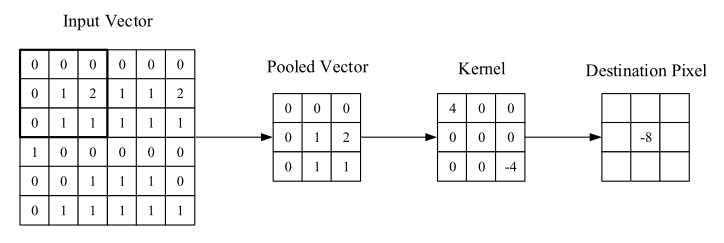
\includegraphics[width=12cm]{../img/bab2/convlayer.PNG}
            \caption{Cara kerja filter pada \textit{convolutional layer}}
            \label{fig:conv}
            Sumber: \citep{OShea2015}
        \end{center}
    \end{figure}

    Pada YOLOv7, setiap operasi konvolusi selalu diikuti dengan \textit{batch normalization} dan fungsi aktivasi \textit{Sigmoid-weighted Linear Unit} sehingga dinamakan CBS (\textit{Convolution}, \textit{Batch normalization}, \textit{Sigmoid-weighted linear unit}) pada arsitektur YOLOv7. YOLOv7 menggunakan 3 jenis operasi konvolusi, yaitu operasi konvolusi dengan $f=1\times 1$ dan $s=1$, operasi konvolusi dengan $f=3\times 3$ dan $s=1$, dan operasi konvolusi dengan $f=3\times 3$ dan $s=2$. Operasi konvolusi dengan $f=1\times 1$ dan $s=1$ bertujuan untuk mengurangi dimensi \textit{feature map}. Operasi konvolusi dengan $f=3\times 3$ dan $s=1$ bertujuan untuk melakukan \textit{feature learning}. Operasi konvolusi dengan $f=3\times 3$ dan $s=2$ bertujuan untuk mengurangi ukuran \textit{feature map}. Arsitektur CBS seperti terlihat pada Gambar \ref{fig:cbs}.

    \begin{figure}[H]
        \begin{center}
            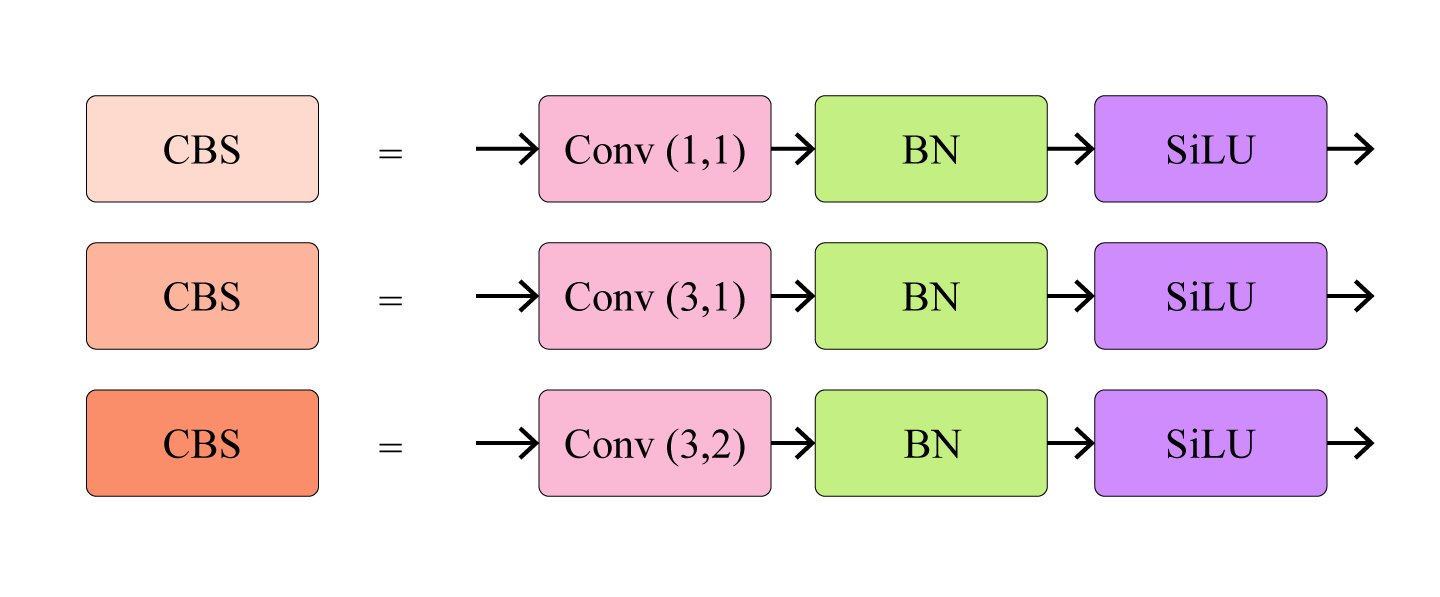
\includegraphics[width=8cm]{../img/bab2/cbs.png}
            \caption{Susunan arsitektur CBS pada YOLOv7}
            \label{fig:cbs}
            Sumber: \citep{Wang2022}
        \end{center}
    \end{figure}

    \subsection{\textit{Pooling Layer}}
    \textit{Feature map} dari \textit{convolutional layer} diproses oleh \textit{pooling layer}. \textit{Pooling layer} berguna untuk mengurangi ukuran \textit{feature map} tanpa menghilangkan informasi yang dibutuhkan. \textit{Pooling layer} yang sering digunakan pada CNN adalah \textit{max pooling} dan \textit{average pooling}. YOLO-v7 menggunakan \textit{max pooling} dalam arsitekturnya. \textit{Max pooling} mengambil nilai tertinggi pada \textit{feature map} berdasarkan ukuran filter. Perhitungan \textit{max pooling} seperti terlihat pada Persamaan \ref{eq:max-pool} dimana $i=0, \cdots, n;j=0, \cdots, n$. Hasil aktivasi \textit{layer} $l$ adalah $h_{l(x,y)}$ dengan $xy$ yang merepresentasikan baris dan kolom. Proses \textit{max pooling} seperti terlihat pada Gambar \ref{fig:max-pool}.

    \begin{align}
        \label{eq:max-pool}
        h_{l(x,y)} &= max_{ij}(h_{(l-1)_{(x+i)(y+j)}})
    \end{align}

    \begin{figure}[H]
        \centering
        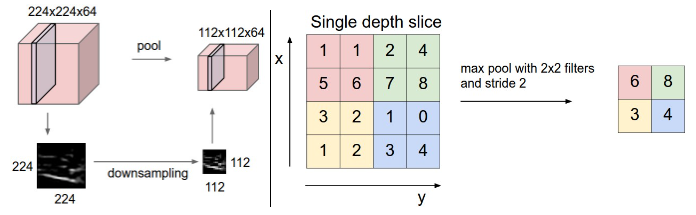
\includegraphics[width=10cm]{../img/bab2/maxpool.png}
        \caption{Cara kerja \textit{max pooling} yang digunakan pada YOLO-v7}
        \label{fig:max-pool}
        Sumber: \citep{Yani2019}
    \end{figure}

    \textit{Max pooling} pada arsitektur YOLOv7 memiliki susunan arsitektur dengan mengombinasikan CBS untuk mengurangi dimensi \textit{feature map} dan melakukan proses \textit{feature learning} seperti terlihat pada Gambar \ref{fig:mp}.

    \begin{figure}[H]
        \begin{center}
            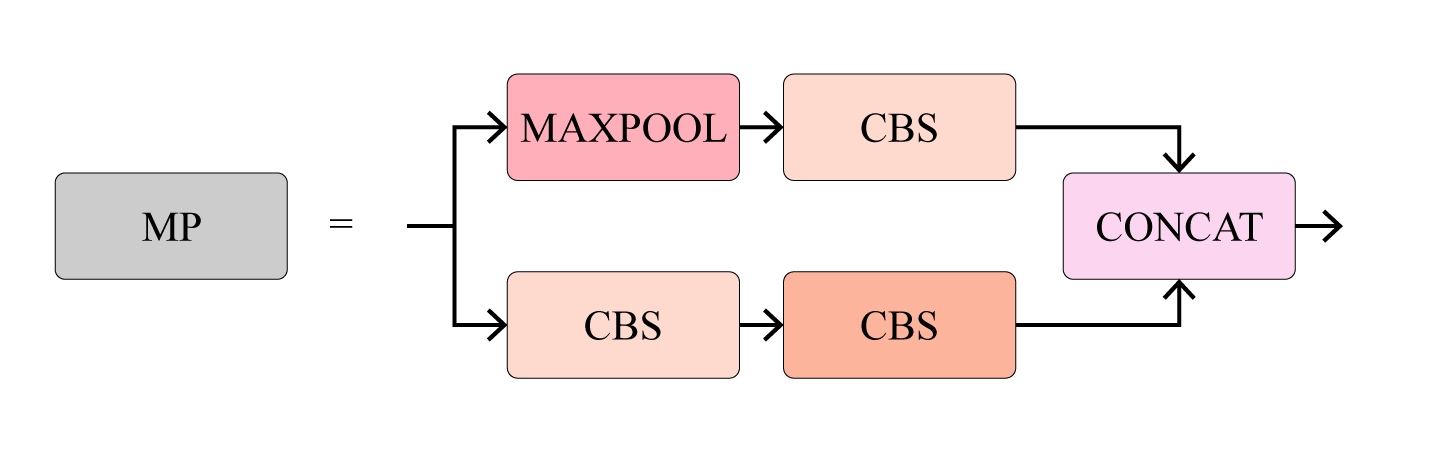
\includegraphics[width=8cm]{../img/bab2/mp.png}
            \caption{Susunan arsitektur MP pada YOLOv7}
            \label{fig:mp}
            Sumber: \citep{Wang2022}
        \end{center}
    \end{figure}

    \subsection{\textit{Upsample Layer}}
    \textit{Upsample layer} merupakan \textit{layer} yang dapat meningkatkan ukuran \textit{feature map}. \textit{Layer} ini mengembalikan ukuran seperti yang digunakan pada \textit{layer} sebelumnya. Rumus untuk mengimplementasikan \textit{upsample layer} seperti terlihat pada Persamaan \ref{eq:upsample} dimana $R$ dan $C$ merupakan tinggi dan lebar data asli sedangkan $R'$ dan $C'$ merupakan tinggi dan lebar data setelah \textit{upsampling}. 

    \begin{align}
        \label{eq:upsample}
        S_r &= \frac{R-1}{R'}\nonumber\\
        S_c &= \frac{C-1}{C'}
    \end{align}

    YOLOv7 menggunakan metode \textit{nearest} untuk mengimplementasikan \textit{upsample layer} pada arsitekturnya. Metode \textit{nearest} adalah cara mengisi data kosong dengan mempertimbangkan nilai di sekitarnya. Proses \textit{upsample} menggunakan metode \textit{nearest} seperti terlihat pada Gambar \ref{fig:il-nearest}.

    \begin{figure}[H]
        \begin{center}
            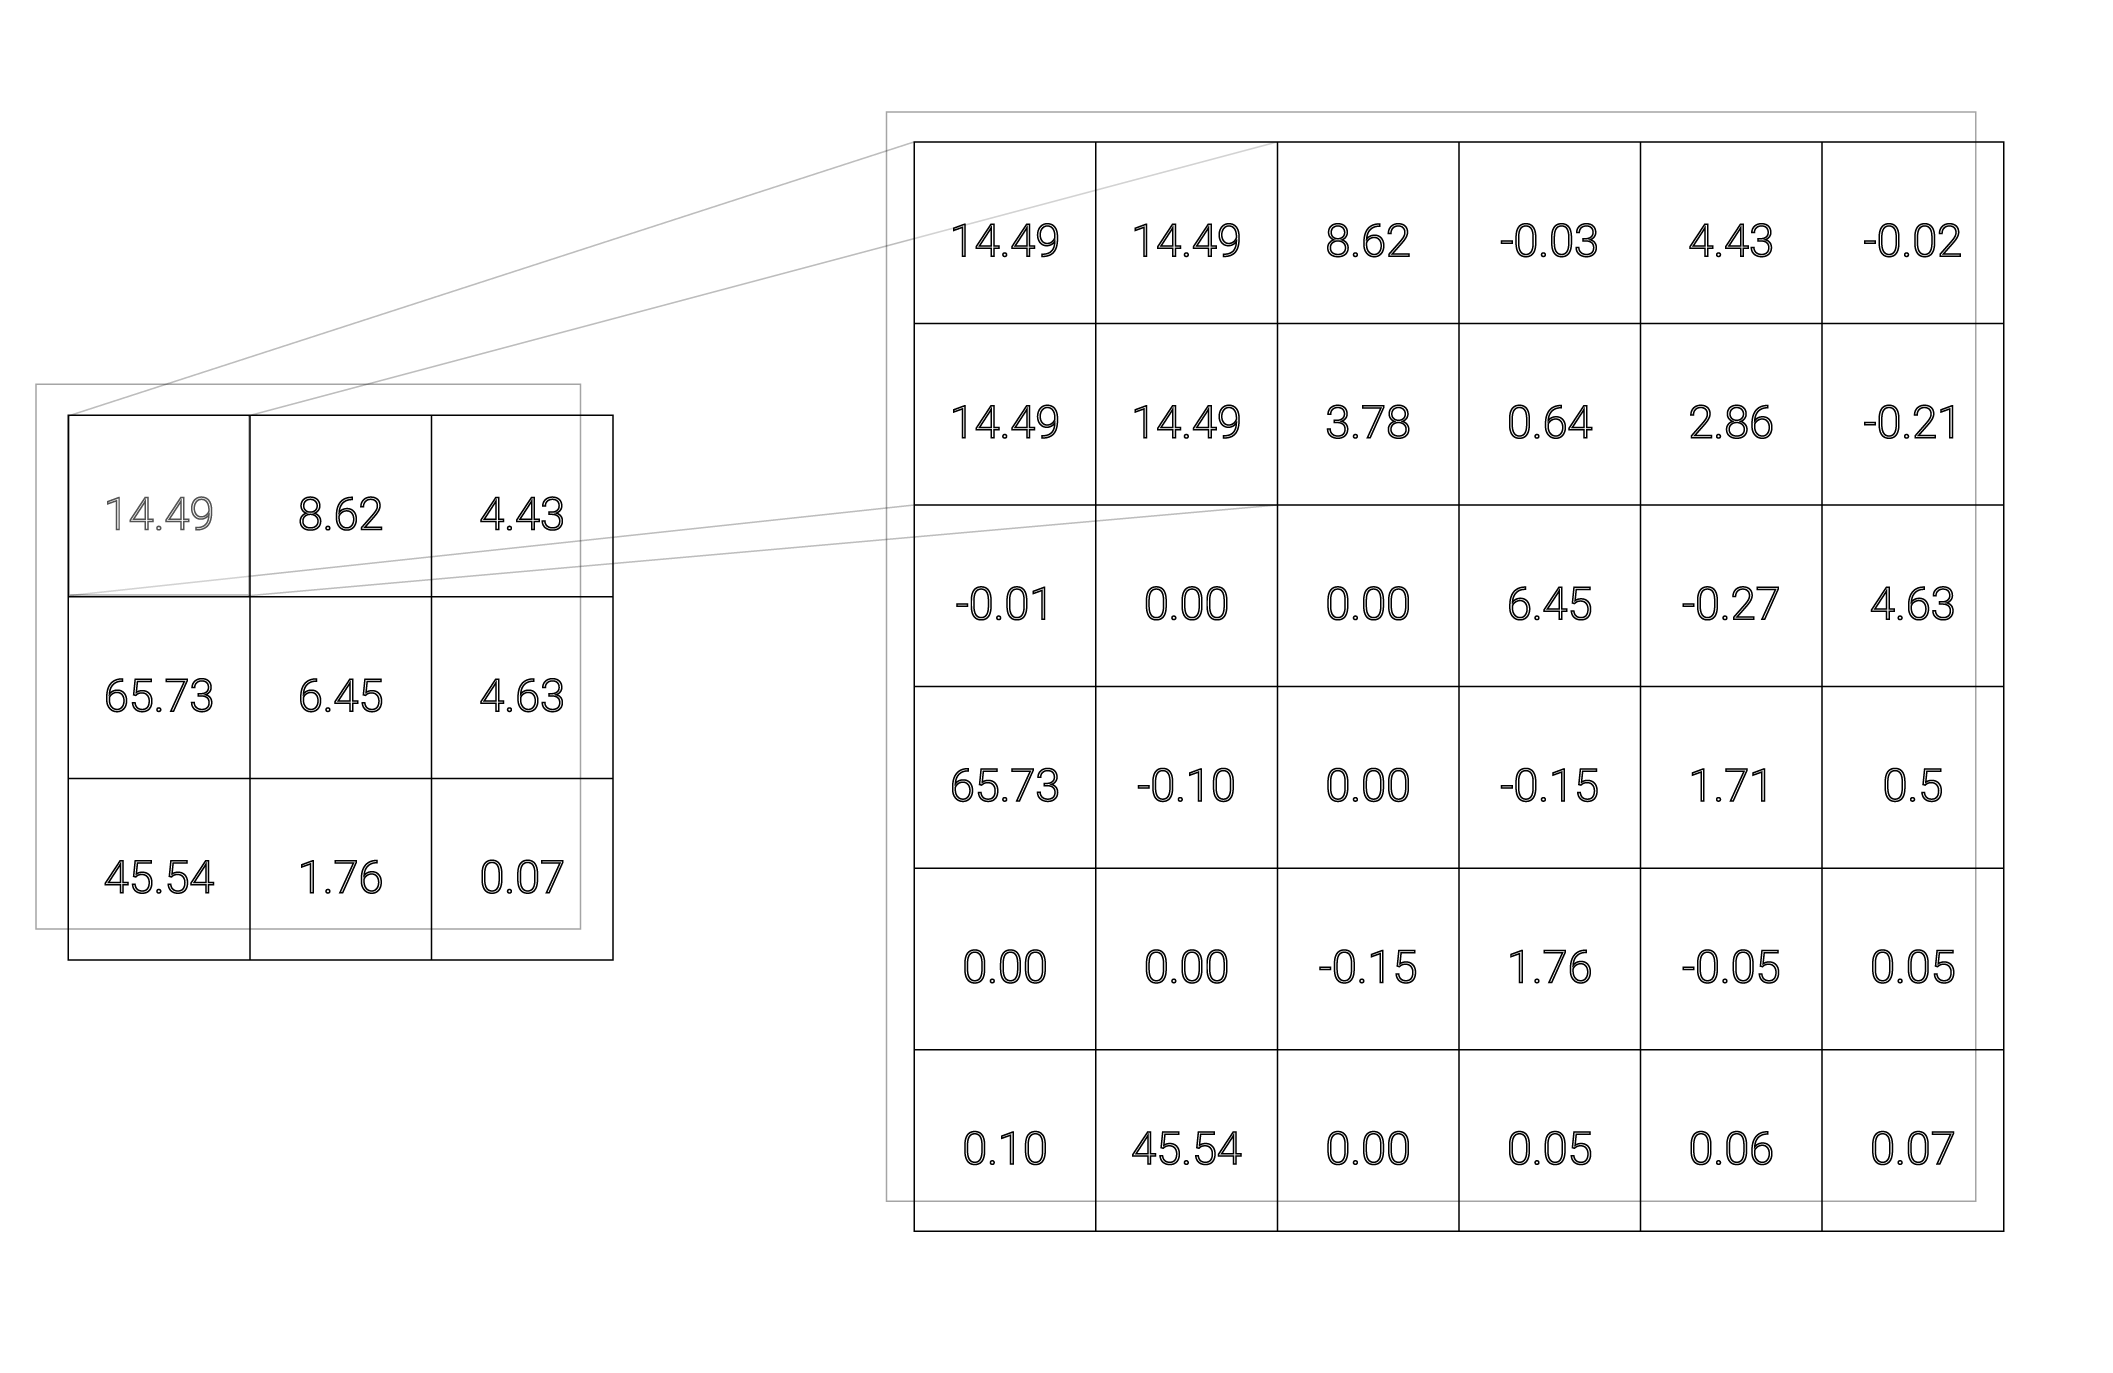
\includegraphics[width=12cm]{../img/bab2/nearest.png}
            \caption{Proses \textit{upsample} pada YOLOv7}
            \label{fig:il-nearest}
        \end{center}
    \end{figure}

    Pada YOLOv7, \textit{upsample layer} dikombinasikan dengan CBS seperti terlihat pada Gambar \ref{fig:up}. Sebelum dilakukan \textit{upsample}, \textit{feature map} melewati CBS terlebih dahulu. Hal ini bertujuan untuk mengurangi dimensi \textit{feature map}.

    \begin{figure}[H]
        \begin{center}
            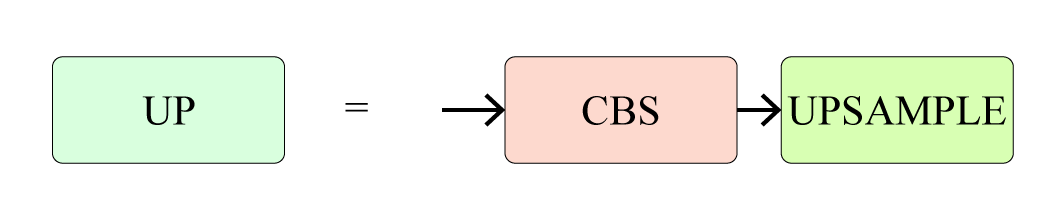
\includegraphics[width=8cm]{../img/bab2/up.png}
            \caption{Susunan arsitektur UP pada YOLOv7}
            \label{fig:up}
            Sumber: \citep{Wang2022}
        \end{center}
    \end{figure}    

    \subsection{\textit{Batch Normalization} (BN)}
    Pada umumnya, hampir setiap metode \textit{deep learning} mengimplementasikan BN. BN merupakan teknik yang dapat mempercepat proses pelatihan model dan membuat proses pelatihan lebih stabil. Teknik ini melakukan normalisasi vektor pada \textit{hidden layers} menggunakan rata-rata dan varian. BN dapat dilakukan sebelum atau sesudah menjalankan fungsi non-linier. Pada setiap \textit{hidden layer}, BN mengubah nilai pada \textit{hidden layer} menggunakan Persamaan \ref{eq:bn-1}-\ref{eq:bn-4}.

    \begin{align}
        \label{eq:bn-1}
        \mu &= \frac{1}{n} \sum_i Z_{i}\\
        \label{eq:bn-2}
        \sigma^2 &= \frac{1}{n} \sum_i (Z_{i}-\mu)^2\\
        \label{eq:bn-3}
        Z_{norm} &= \frac{Z_{i}-\mu}{\sqrt{\sigma^2-\epsilon}}\\
        \label{eq:bn-4}
        \breve{Z} &= \gamma \ast Z_{norm}+\beta
    \end{align}

    Pertama, BN menghitung nilai rata-rata dan varian menggunakan Persamaan \ref{eq:bn-1} dan \ref{eq:bn-2}. Kemudian dilakukan normalisasi menggunakan Persamaan \ref{eq:bn-3} sehingga data keluaran berdistribusi normal dimana $\epsilon = 2.71828$ untuk stabilitas numerik. Langkah terakhir menghitung keluaran $\breve{Z}$ dengan menerapkan transformasi linier terhadap $\gamma$ dan $\beta$ seperti Persamaan \ref{eq:bn-4}.

    \subsection{\textit{Leaky Rectified Linear Unit} (Leaky ReLU)}
    ReLU seringkali digunakan pada masalah \textit{deep learning} terutama pada \textit{computer vision}. ReLU memiliki tingkat konvergensi yang lebih baik daripada fungsi aktivasi $\sigma$ (\textit{sigmoid}) dan $tanh$. Hasil keluaran ReLU memiliki ambang batas $0$ sehingga jaringan lebih cepat karena memiliki perhitungan yang efisien. Akan tetapi, ReLU memiliki masalah \textit{dying ReLU} dimana ReLU tidak berfungsi untuk semua data masukan karena bernilai kurang dari nol. Berawal dari hal ini, Leaky ReLU muncul dengan mengubah gradien ReLU sedikit ke kiri sehingga Leaky ReLU dapat menghasilkan beberapa nilai jika data masukan kurang dari nol. Rumus Leaky ReLU seperti terlihat pada Persamaan \ref{eq:l-relu}. Grafik Leaky ReLU seperti terlihat pada Gambar \ref{fig:l-relu} \citep{Xu2015}.

    \begin{align}
        \label{eq:l-relu}
        f(x) &= max(0.1x, x)
    \end{align}

    \begin{figure}[H]
        \begin{center}
            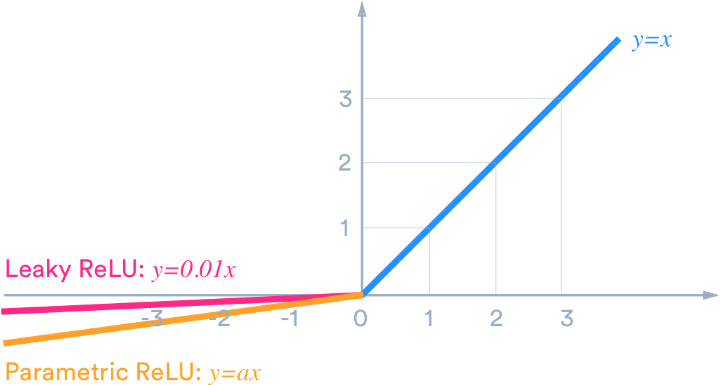
\includegraphics[width=8cm]{../img/bab2/lrelu.png}
            \caption{Grafik Leaky ReLU}
            \label{fig:l-relu}
            Sumber: \citep{Xu2015}
        \end{center}
    \end{figure}

    \subsection{\textit{Sigmoid-weighted Linear Unit} (SiLU)}
    SiLU merupakan salah satu fungsi aktivasi yang diusulkan untuk \textit{reinforcement learning}. Fungsi aktivasi SiLU dihitung dengan melakukan operasi perkalian antara fungsi sigmoid dengan data masukan. Rumus SiLU seperti terlihat pada Persamaan \ref{eq:silu}. Grafik SiLU tidak menaik secara monoton seperti ReLU, akan tetapi sedikit melandai ke bawah dengan nilai minimum sekitar $-0.28$ untuk $z_k \approx -1.28$. Grafik SiLU seperti terlihat pada Gambar \ref{fig:silu}.

    \begin{align}
        \label{eq:silu}
        a_k(z_k) &= z_k\sigma (z_k)\nonumber\\
        &= z_k\frac{1}{1+e^{-(z_k)}}
    \end{align}

    \begin{figure}[H]
        \begin{center}
            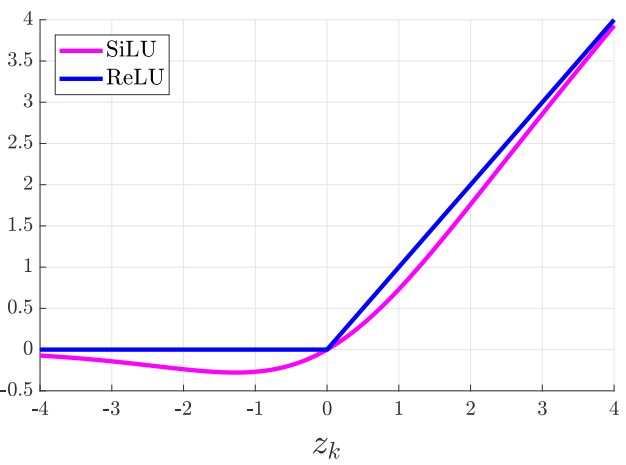
\includegraphics[width=8cm]{../img/bab2/silu.PNG}
            \caption{Perbandingan grafik SiLU dan ReLU}
            \label{fig:silu}
            Sumber: \citep{Elfwing2018}
        \end{center}
    \end{figure}

    % TODO: Turunan dari activation function masukkan ke dalam BAB II

\section{\textit{You Only Look Once version 7} (YOLO-v7)}
YOLO merupakan algoritma deteksi objek berdasarkan \textit{Fully Connected Neural Network} (FCNN). Algoritma ini dapat digunakan untuk mendeteksi objek secara \textit{real-time}. Algoritma ini bekerja dengan membagi citra ke dalam beberapa kisi. Setiap kisi pada YOLO memiliki kemampuan untuk memprediksi \textit{bounding box} dan kelas di dalamnya. \textit{Bounding box} merupakan kotak pembatas yang menandakan di dalamnya terdapat objek tertentu. Objek tersebut kemudian diklasifikasikan ke dalam kelas tertentu dengan memilih batas kotak yang memiliki nilai IoU paling tinggi. Secara umum, terdapat tiga komponen utama pada YOLO, yaitu \textit{backbone}, \textit{neck}, dan \textit{head}. \textit{Backbone} melakukan \textit{feature learning} kemudian diteruskan ke \textit{neck}. Bagian \textit{neck} mengumpulkan \textit{feature map} yang dipelajari dari \textit{backbone}. Pada akhirnya, \textit{head} memprediksi \textit{bounding box} dan probabilitas kelas yang ada di dalam \textit{bounding box}. YOLO merupakan metode yang populer dalam bidang \textit{computer vision} dan memunculkan banyak versi. Penelitian ini menggunakan YOLO-v7 dengan arsitektur seperti terlihat pada Gambar \ref{fig:yolov7-archi}.
\begin{figure}[H]
    \begin{center}
        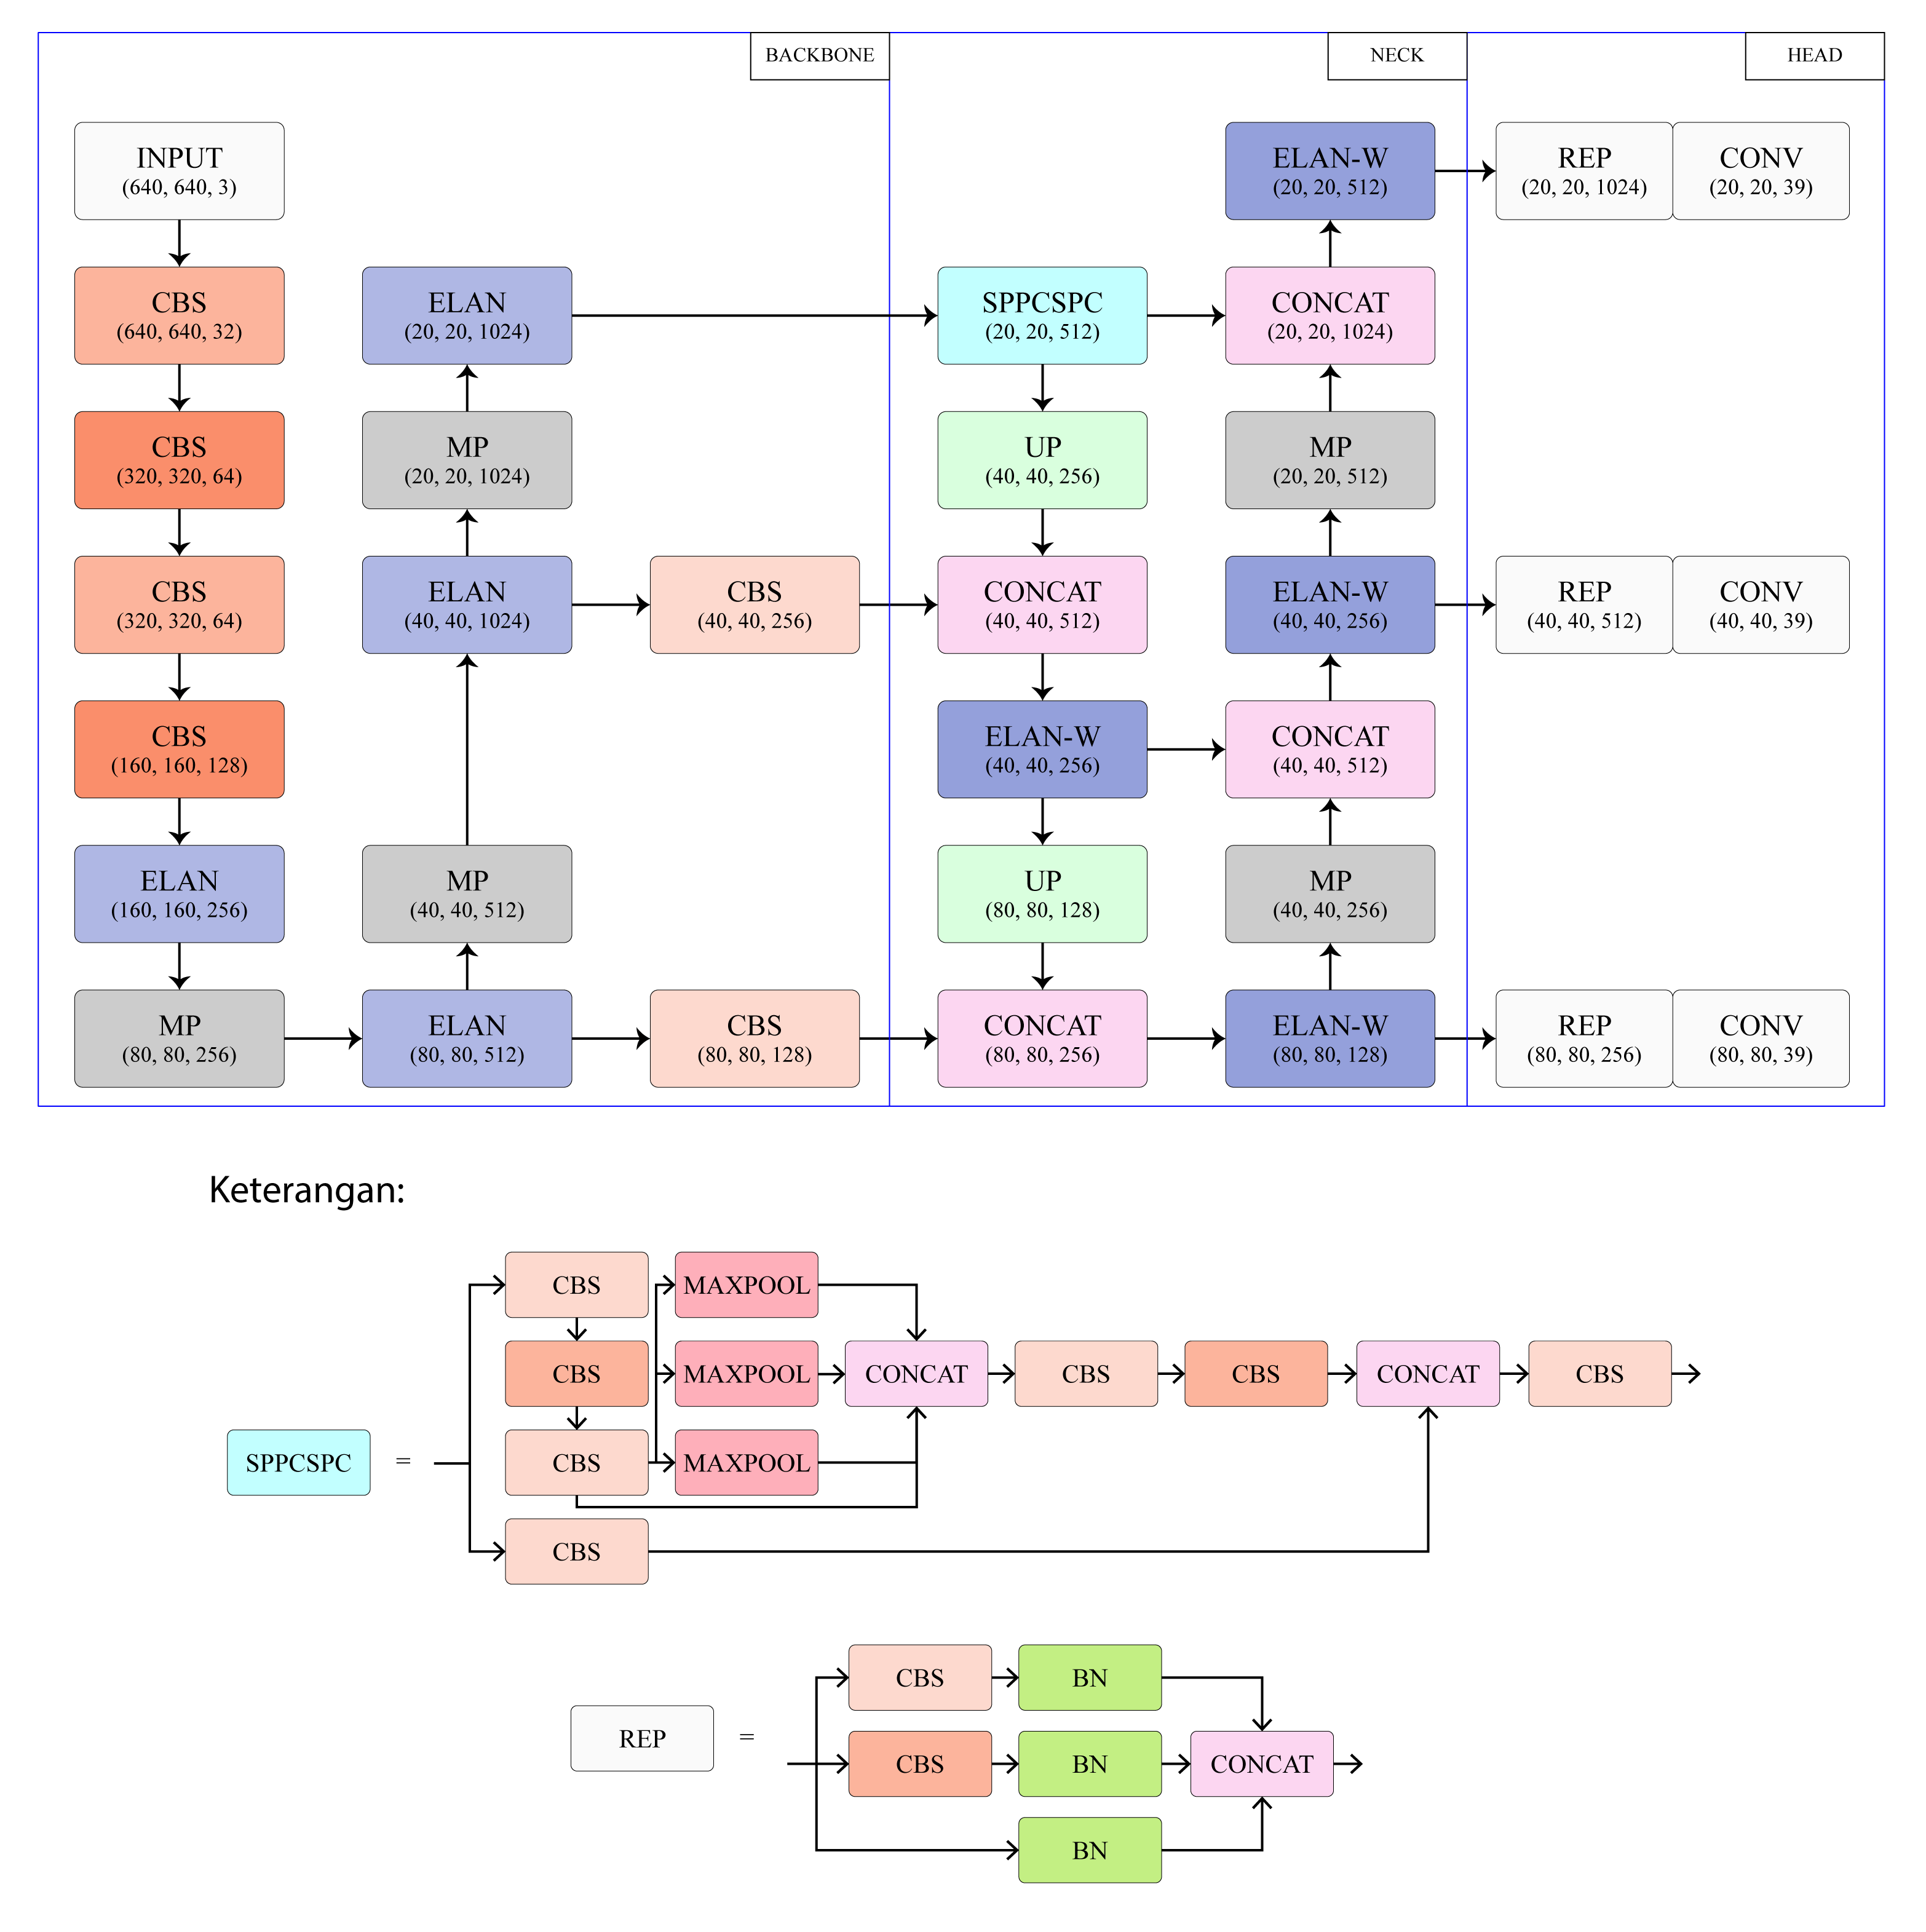
\includegraphics[width=13cm]{../img/bab2/yolov7-architecture.png}
        \caption{Arsitektur YOLO-v7}
        \label{fig:yolov7-archi}
        Sumber: \citep{Wang2022}
    \end{center}
\end{figure}

    \subsection{\textit{Efficient Layer Aggregation Networks} (ELAN)}
    ELAN merupakan jaringan yang melakukan proses agregasi fitur dan transfer fitur. Pada YOLO-v7, ELAN berada pada bagian \textit{backbone} sehingga ELAN bertugas untuk melakukan \textit{feature learning}. Modul ini memiliki struktur jaringan dan proses komputasi pemanfaatan parameter yang efisien sehingga jaringan dapat mempelajari fitur yang lebih beragam. ELAN memiliki dua cabang. Cabang pertama melakukan konvolusi $1\times 1$ untuk mengurangi \textit{depth}. Cabang kedua melakukan konvolusi $1\times 1$ kemudian melalui empat modul konvolusi $3\times 3$ yang berguna untuk \textit{feature learning}. Pada akhirnya, keempat fitur digabungkan untuk mendapatkan fitur akhir. Terdapat dua jenis ELAN, yaitu ELAN dan ELAN-W dimana perbedaan keduanya terdapat pada output yang diteruskan pada cabang kedua. Struktur jaringan ELAN dan ELAN-W seperti terlihat pada Gambar \ref{fig:elan}.

    \begin{figure}[H]
        \centering
        \begin{tabular}{c}
            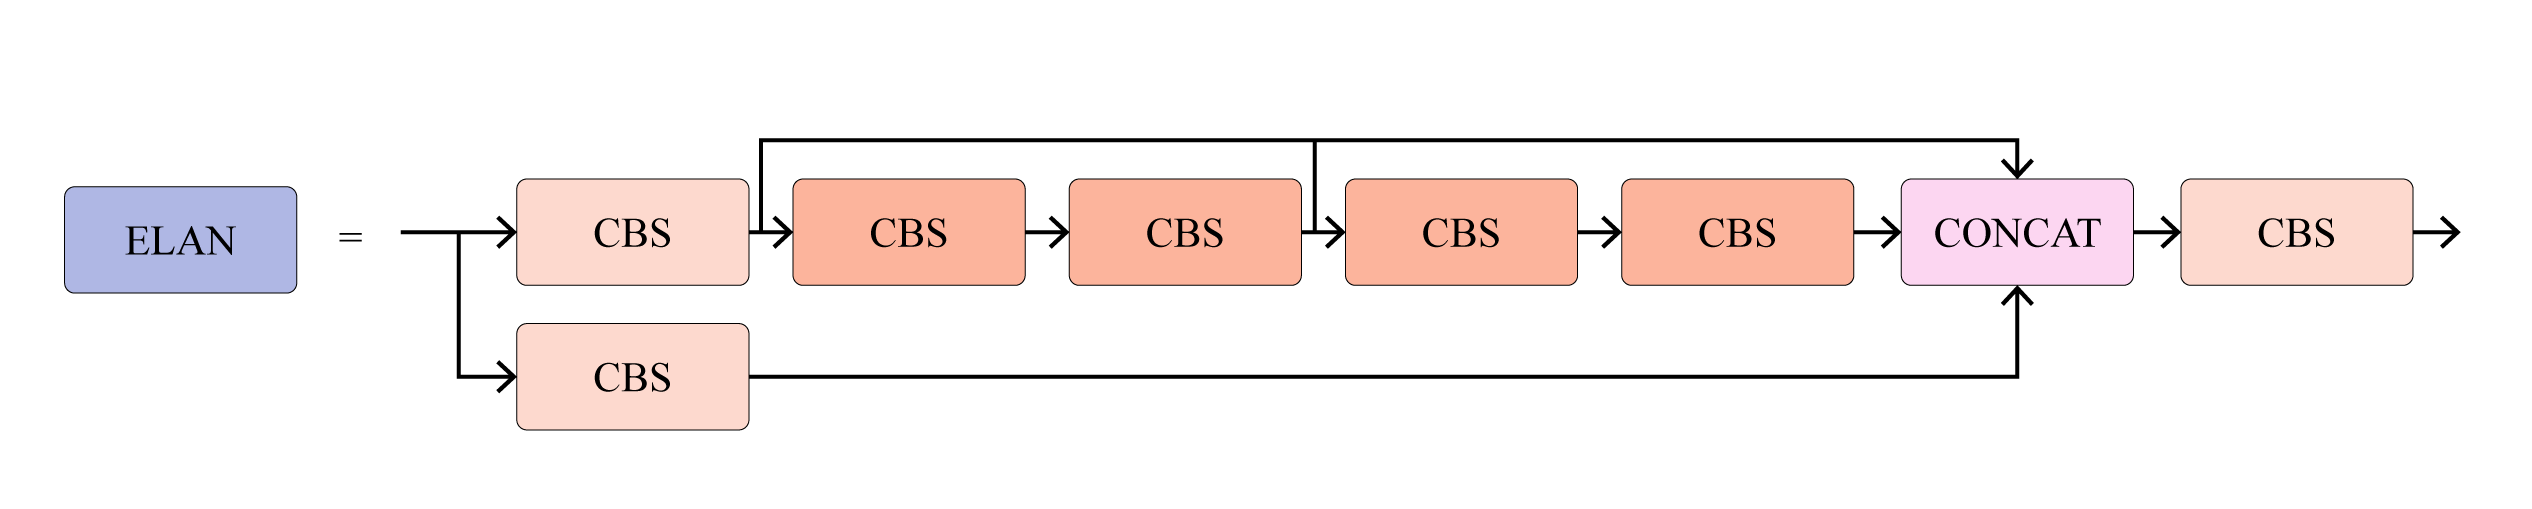
\includegraphics[width=13cm]{../img/bab2/elan.png}\\
            (a)\\
            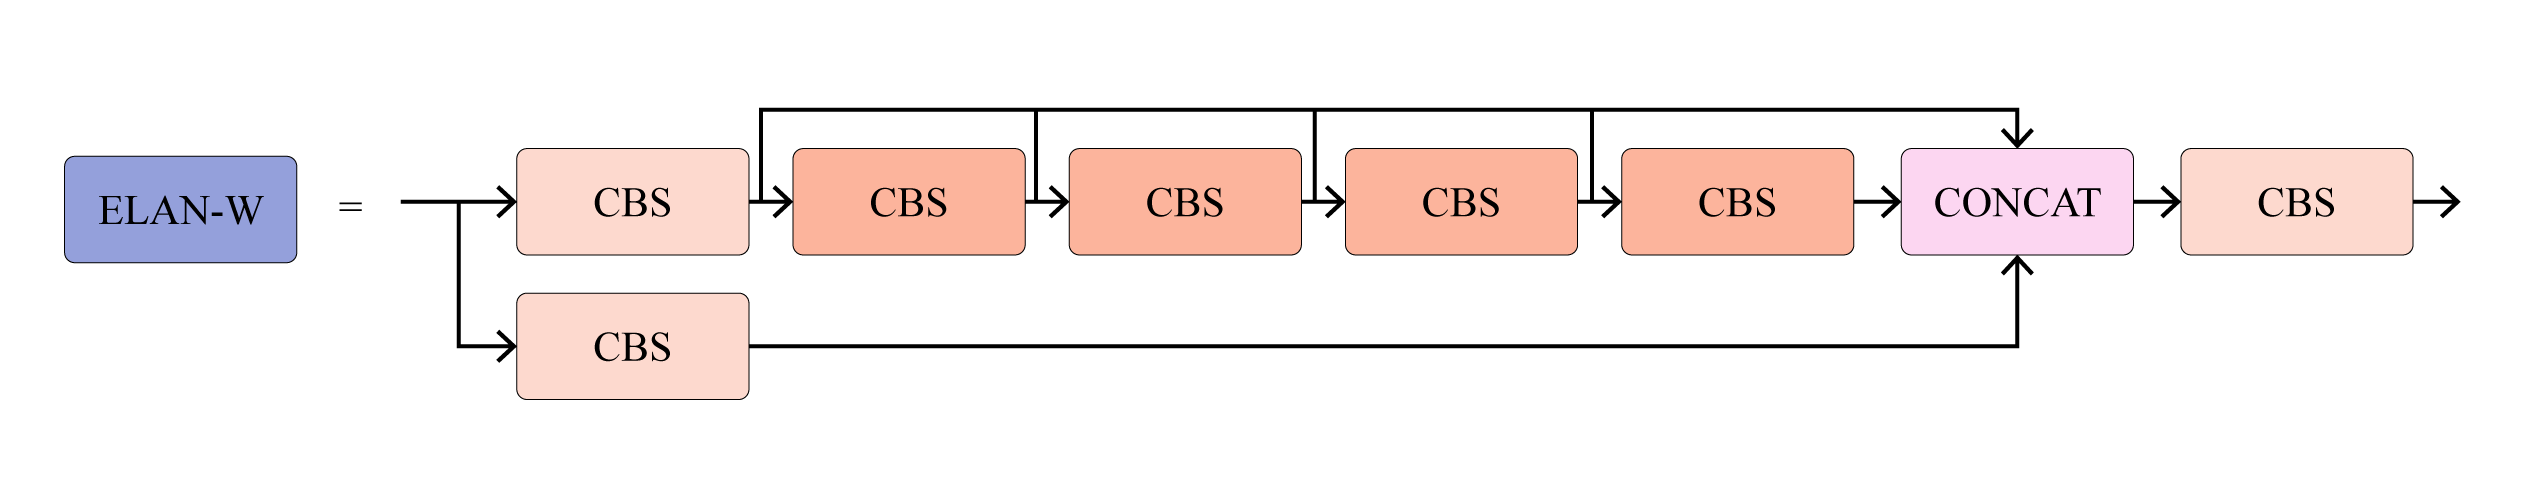
\includegraphics[width=13cm]{../img/bab2/elan-w.png}\\
            (b)\\
        \end{tabular}
        \caption{Struktur jaringan ELAN (a) ELAN; (b) ELAN-W}
        \label{fig:elan}
        Sumber: \citep{Wang2022}
    \end{figure}

\section{\textit{Confusion Matrix}}
\textit{Confusion matrix} adalah tabel yang digunakan untuk menggambarkan performa dari sebuah algoritma klasifikasi \citep{nasution2022sentiment, julianto2021performance}. Secara matematis, \textit{confusion matrix} berupa matrix $C_{ij}$ yang berisi nilai integer yang tidak negatif dengan $i=1, 2, 3, \cdots, n,j=1, 2, 3, \cdots, n$ dimana $n$ merupakan jumlah kelas pada permasalahan klasifikasi. Elemen $C_{ij}$ merupakan hasil klasifikasi selama proses pengujian model. Jika $i=j$ maka kelas $i$ terklasifikasi dengan benar pada kelas $j$. Sehingga dapat dikatakan elemen pada diagonal utama matriks merupakan semua kelas yang terklasifikasi dengan benar. Sedangkan elemen tidak nol lainnya menandakan kesalahan klasifikasi \citep{Susmaga2004}. Setiap elemen pada \textit{confusion matrix} termasuk ke dalam beberapa kategori berikut \citep{Shultz2017}:
\begin{enumerate}
    \item \textit{True Positive} (TP) menunjukkan ketepatan model dalam mengklasifikasikan kelas positif sebagai kelas positif.
    \item \textit{False Positive} (FP) menunjukkan ketepatan model dalam mengklasifikasikan kelas positif sebagai kelas negatif.
    \item \textit{True Negative} (TN) menunjukkan ketepatan model dalam mengklasifikasikan kelas negatif sebagai kelas negatif.
    \item \textit{False Negative} (FN) menunjukkan ketepatan model dalam mengklasifikasikan kelas negatif sebagai kelas positif.
\end{enumerate}

Sehingga \textit{confusion matrix} dapat digambarkan ke dalam sebuah tabel. Tabel \ref{tab:conf-mat} menunjukkan representasi dari \textit{confusion matrix}. Pada Tabel \ref{tab:conf-mat} terdapat $1, 2, 3, \cdots, n$ kelas. Baris dan kolom pada Tabel \ref{tab:conf-mat} berturut-turut merepresentasikan data aktual dan data prediksi.

\begin{table}[H]
    \caption{\textit{Confusion matrix}}
    \centering
    \begin{tblr}{
        rows = {3em, rowsep = 2pt},
        columns = {3em, colsep = 2pt},
        cells = {m,c},
        hlines,
        vlines,
      }
          \multicolumn{2}{c}{ \multirow{2}{*}{} }             &\multicolumn{4}{|c|}{Prediksi}                 \\
                                                              &           &$1$        &$2$        &$\cdots$   &$n$        \\
          \multirow{4}{*}{\rotatebox[origin=c]{90}{Aktual}}   &$1$        &$C_{11}$   &$FN$       &$\cdots$   &$C_{1n}$   \\
                                                              &$2$        &$FP$       &$TP$       &$\cdots$   &$FP$       \\
                                                              &$\vdots$   &$\vdots$   &$\vdots$   &$\ddots$   &$\vdots$   \\
                                                              &$n$        &$C_{n1}$   &$FN$       &$\cdots$   &$C_{nn}$   \\
    \end{tblr}
    \label{tab:conf-mat}\\
    \vspace{2pt}
    Sumber: \citep{Shultz2017}
\end{table}

\section{\textit{Intersection over Union} (IoU)}
IoU merupakan indikasi untuk mengetahui seberapa tepat prediksi kotak pembatas ke terhadap objek yang ada pada citra. Semakin tinggi nilai IoU menandakan semakin baik prediksi kotak pembatas oleh model deteksi objek. Kondisi IoU seperti terlihat pada Gambar \ref{fig:iou-cond} (a) dimana $(x_1, y_1)$ dan $(x_2, y_2)$ merupakan koordinat kotak pembatas data aktual sedangkan $(x_3, y_3)$ dan $(x_4, y_4)$ merupakan koordinat kotak pembatas hasil prediksi.

\begin{figure}[H]
    \centering
    \begin{tabular}{ccc}
        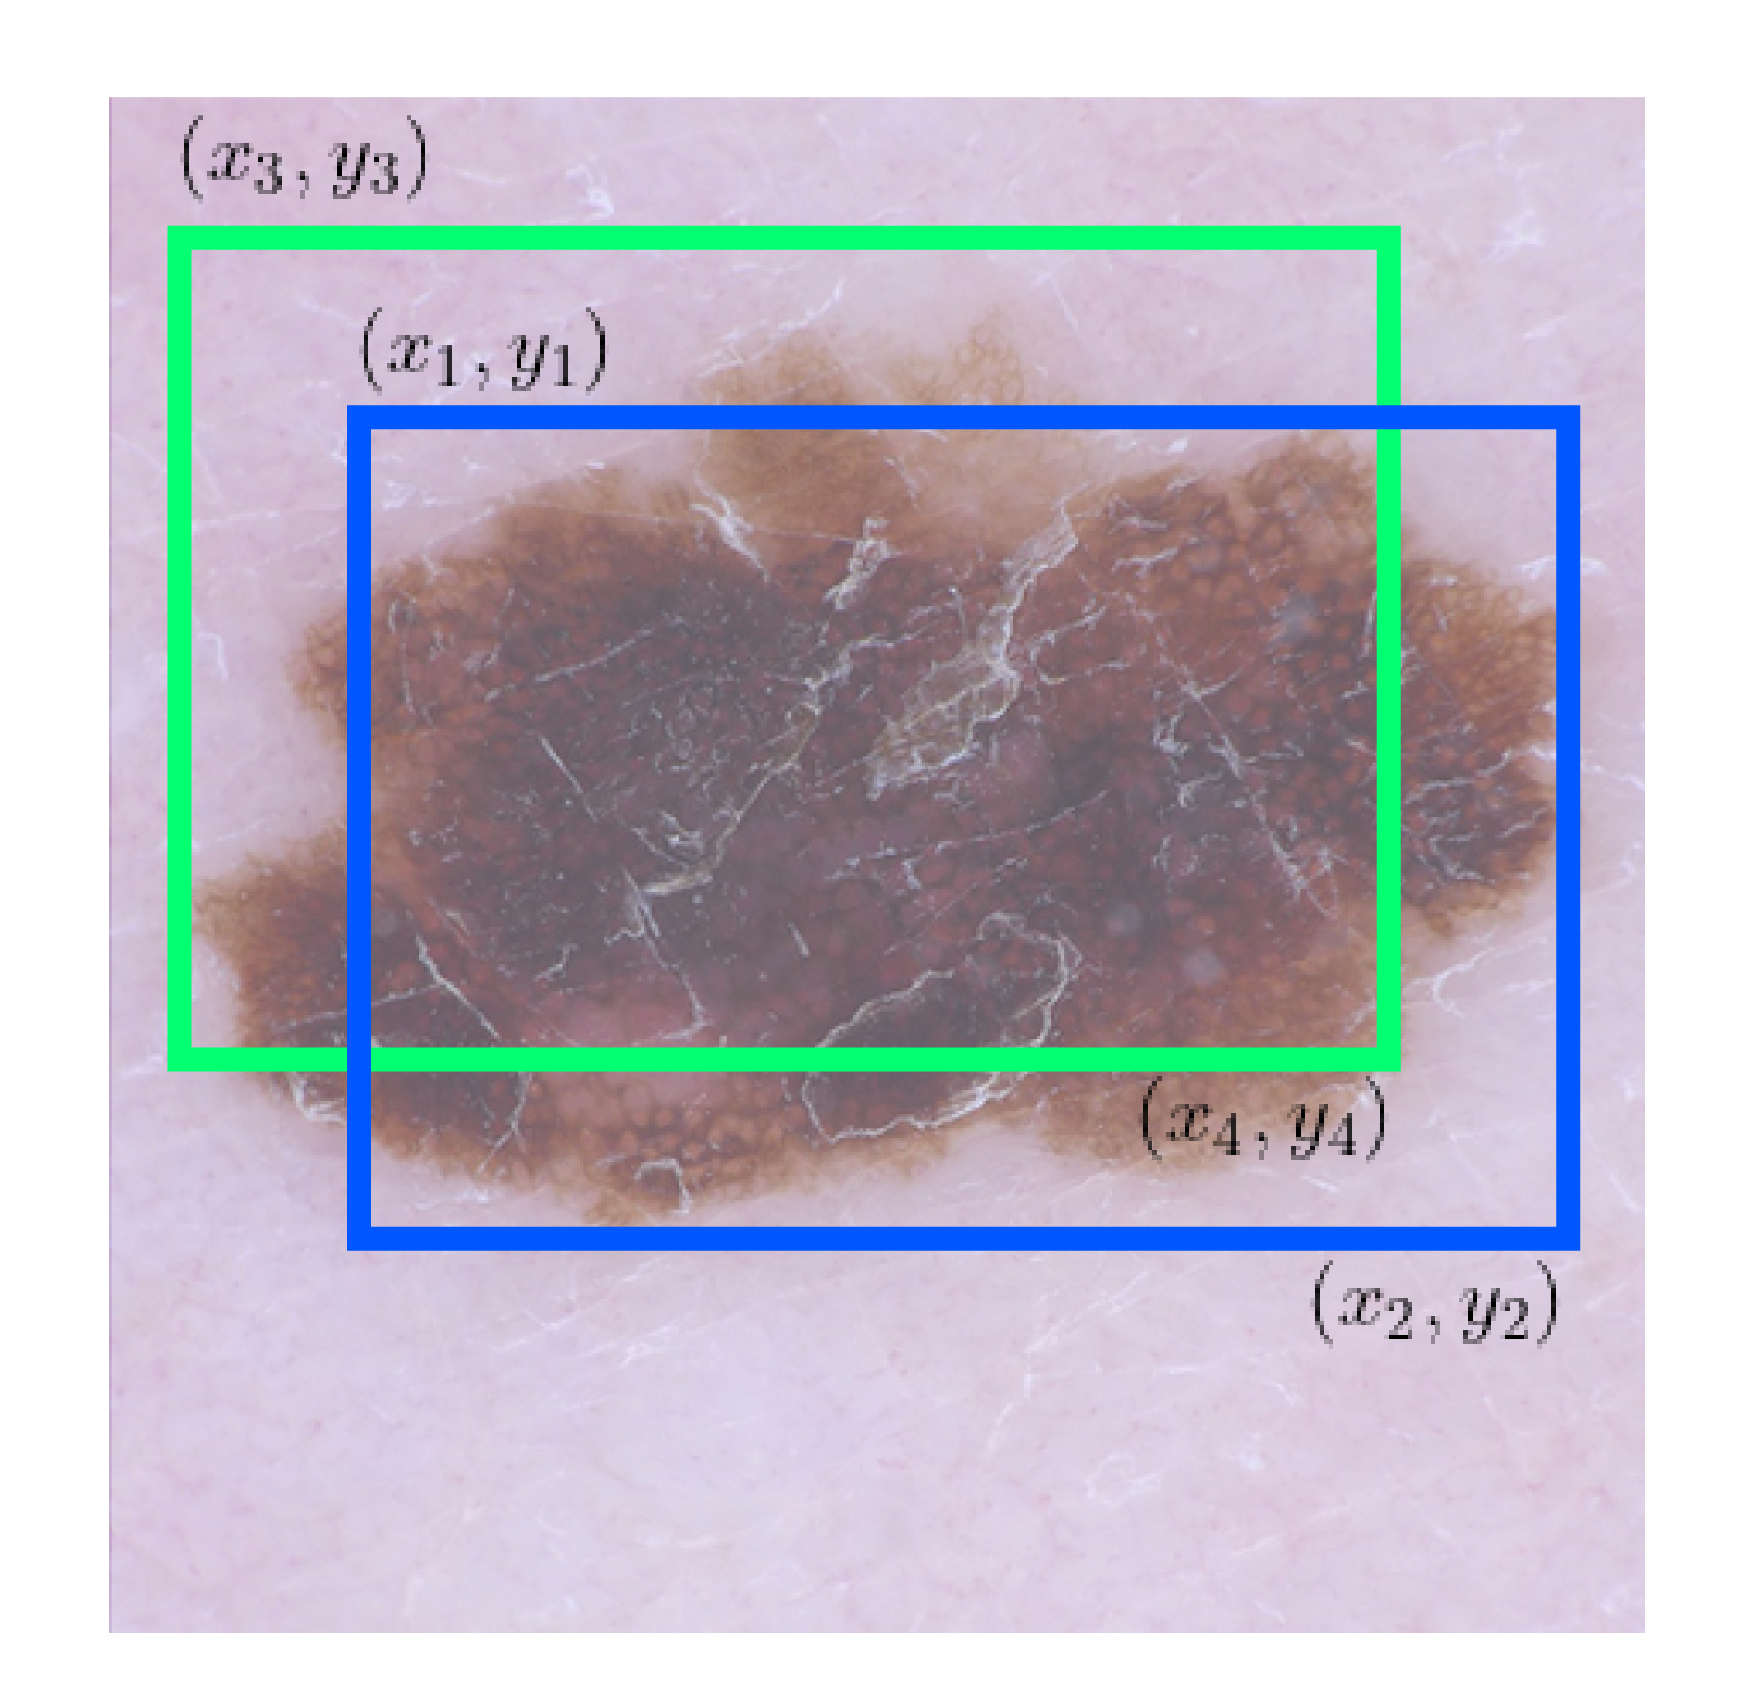
\includegraphics[width=3cm]{../img/bab2/bb-two.png}
        &
        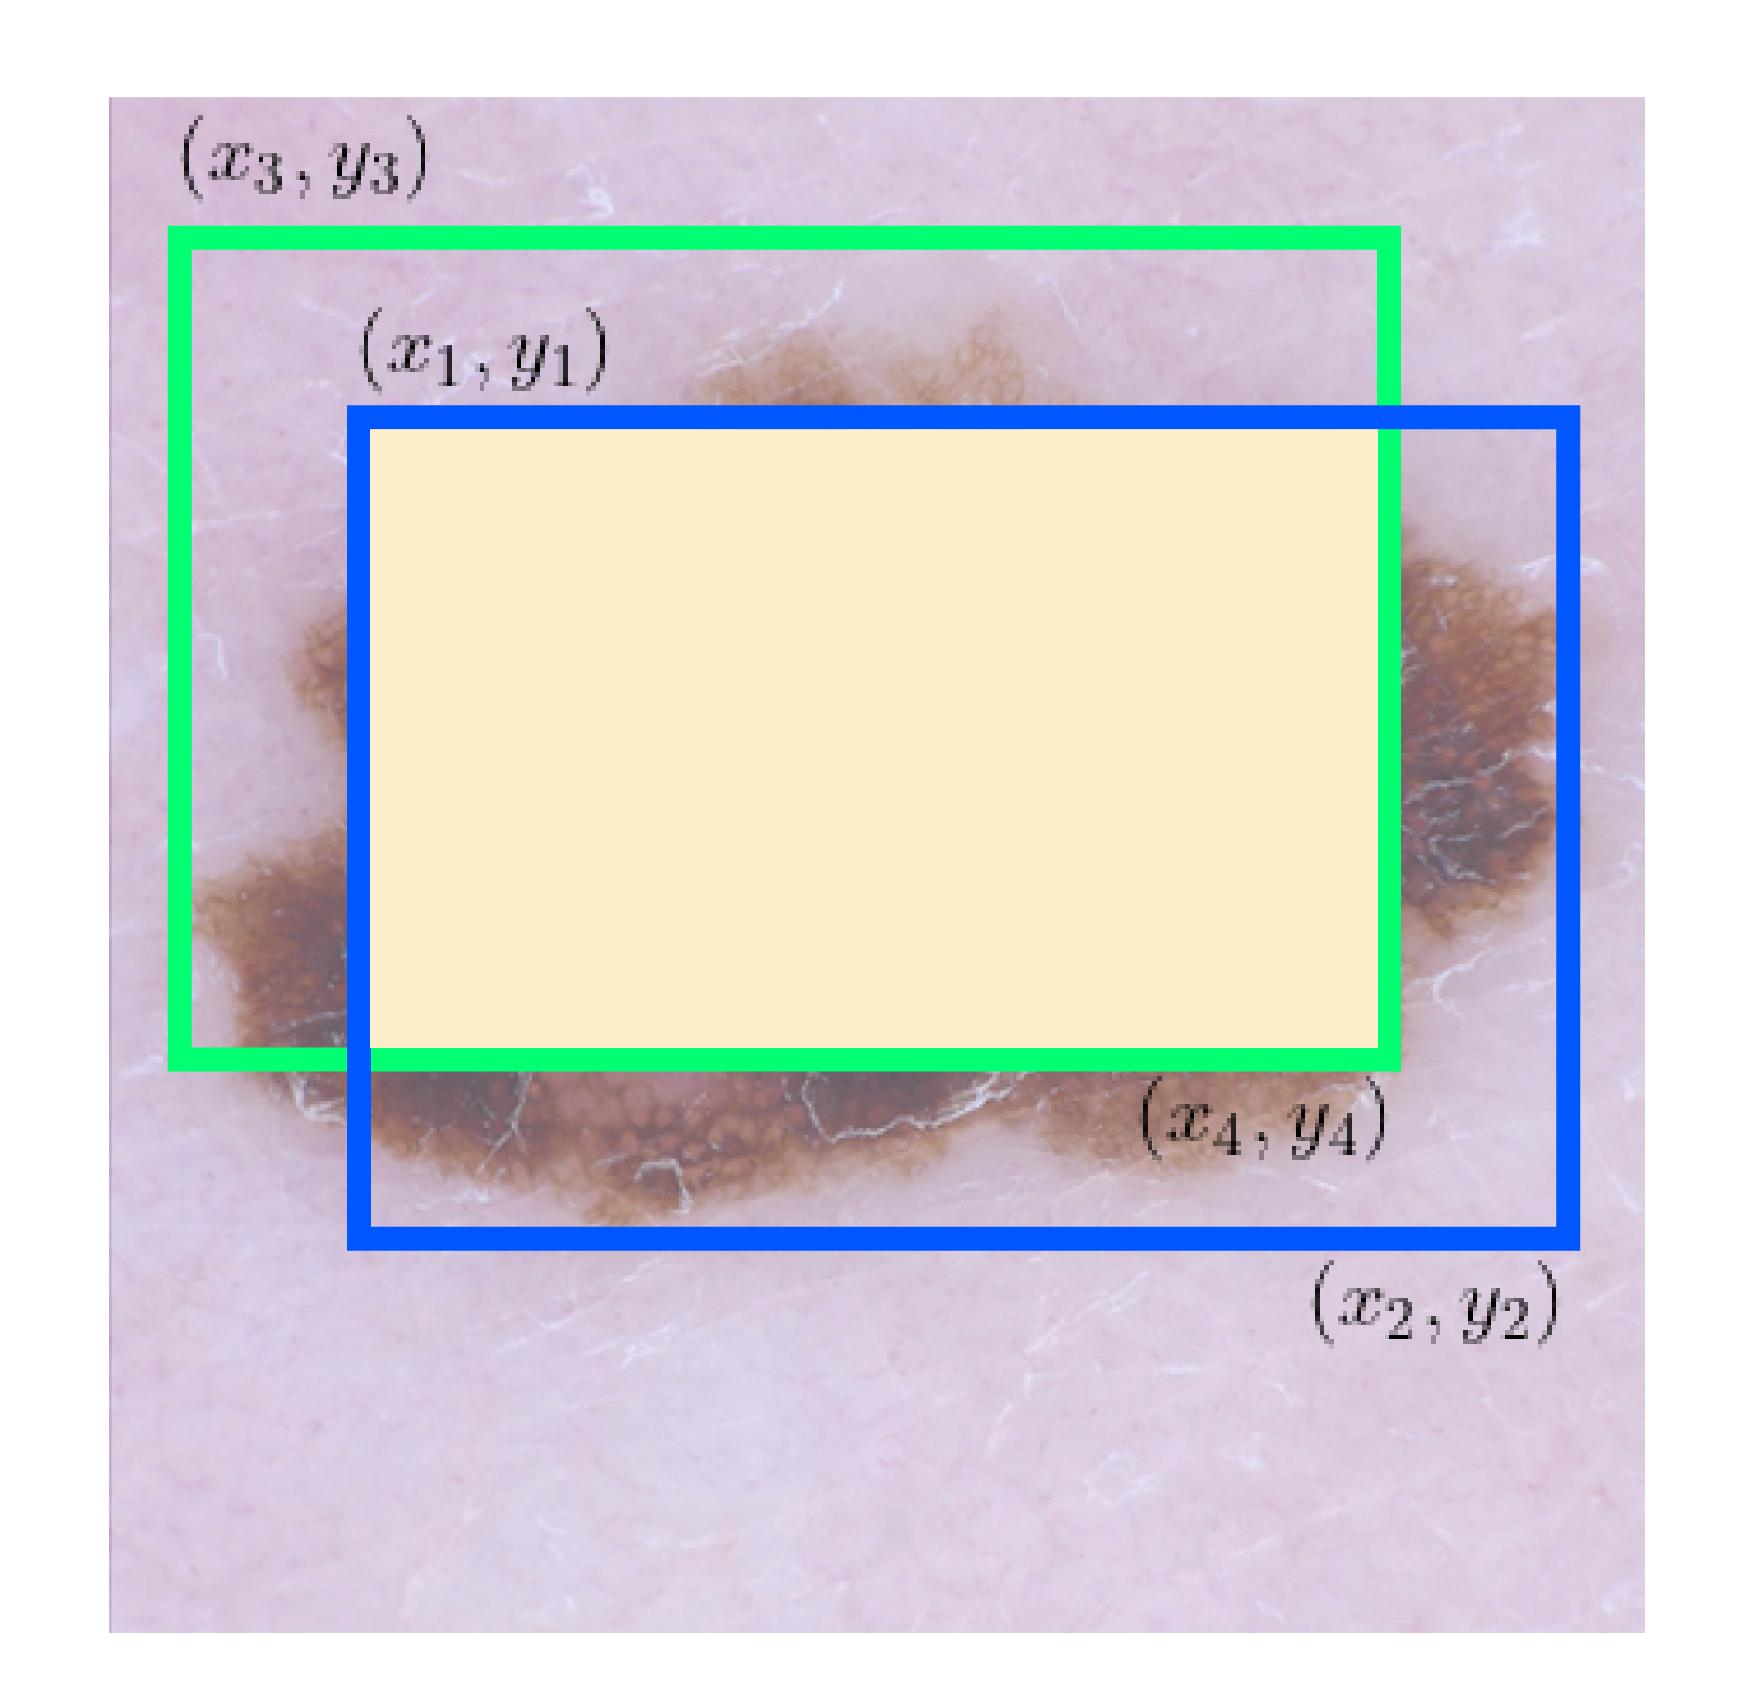
\includegraphics[width=3cm]{../img/bab2/bb-overlap.png}
        &
        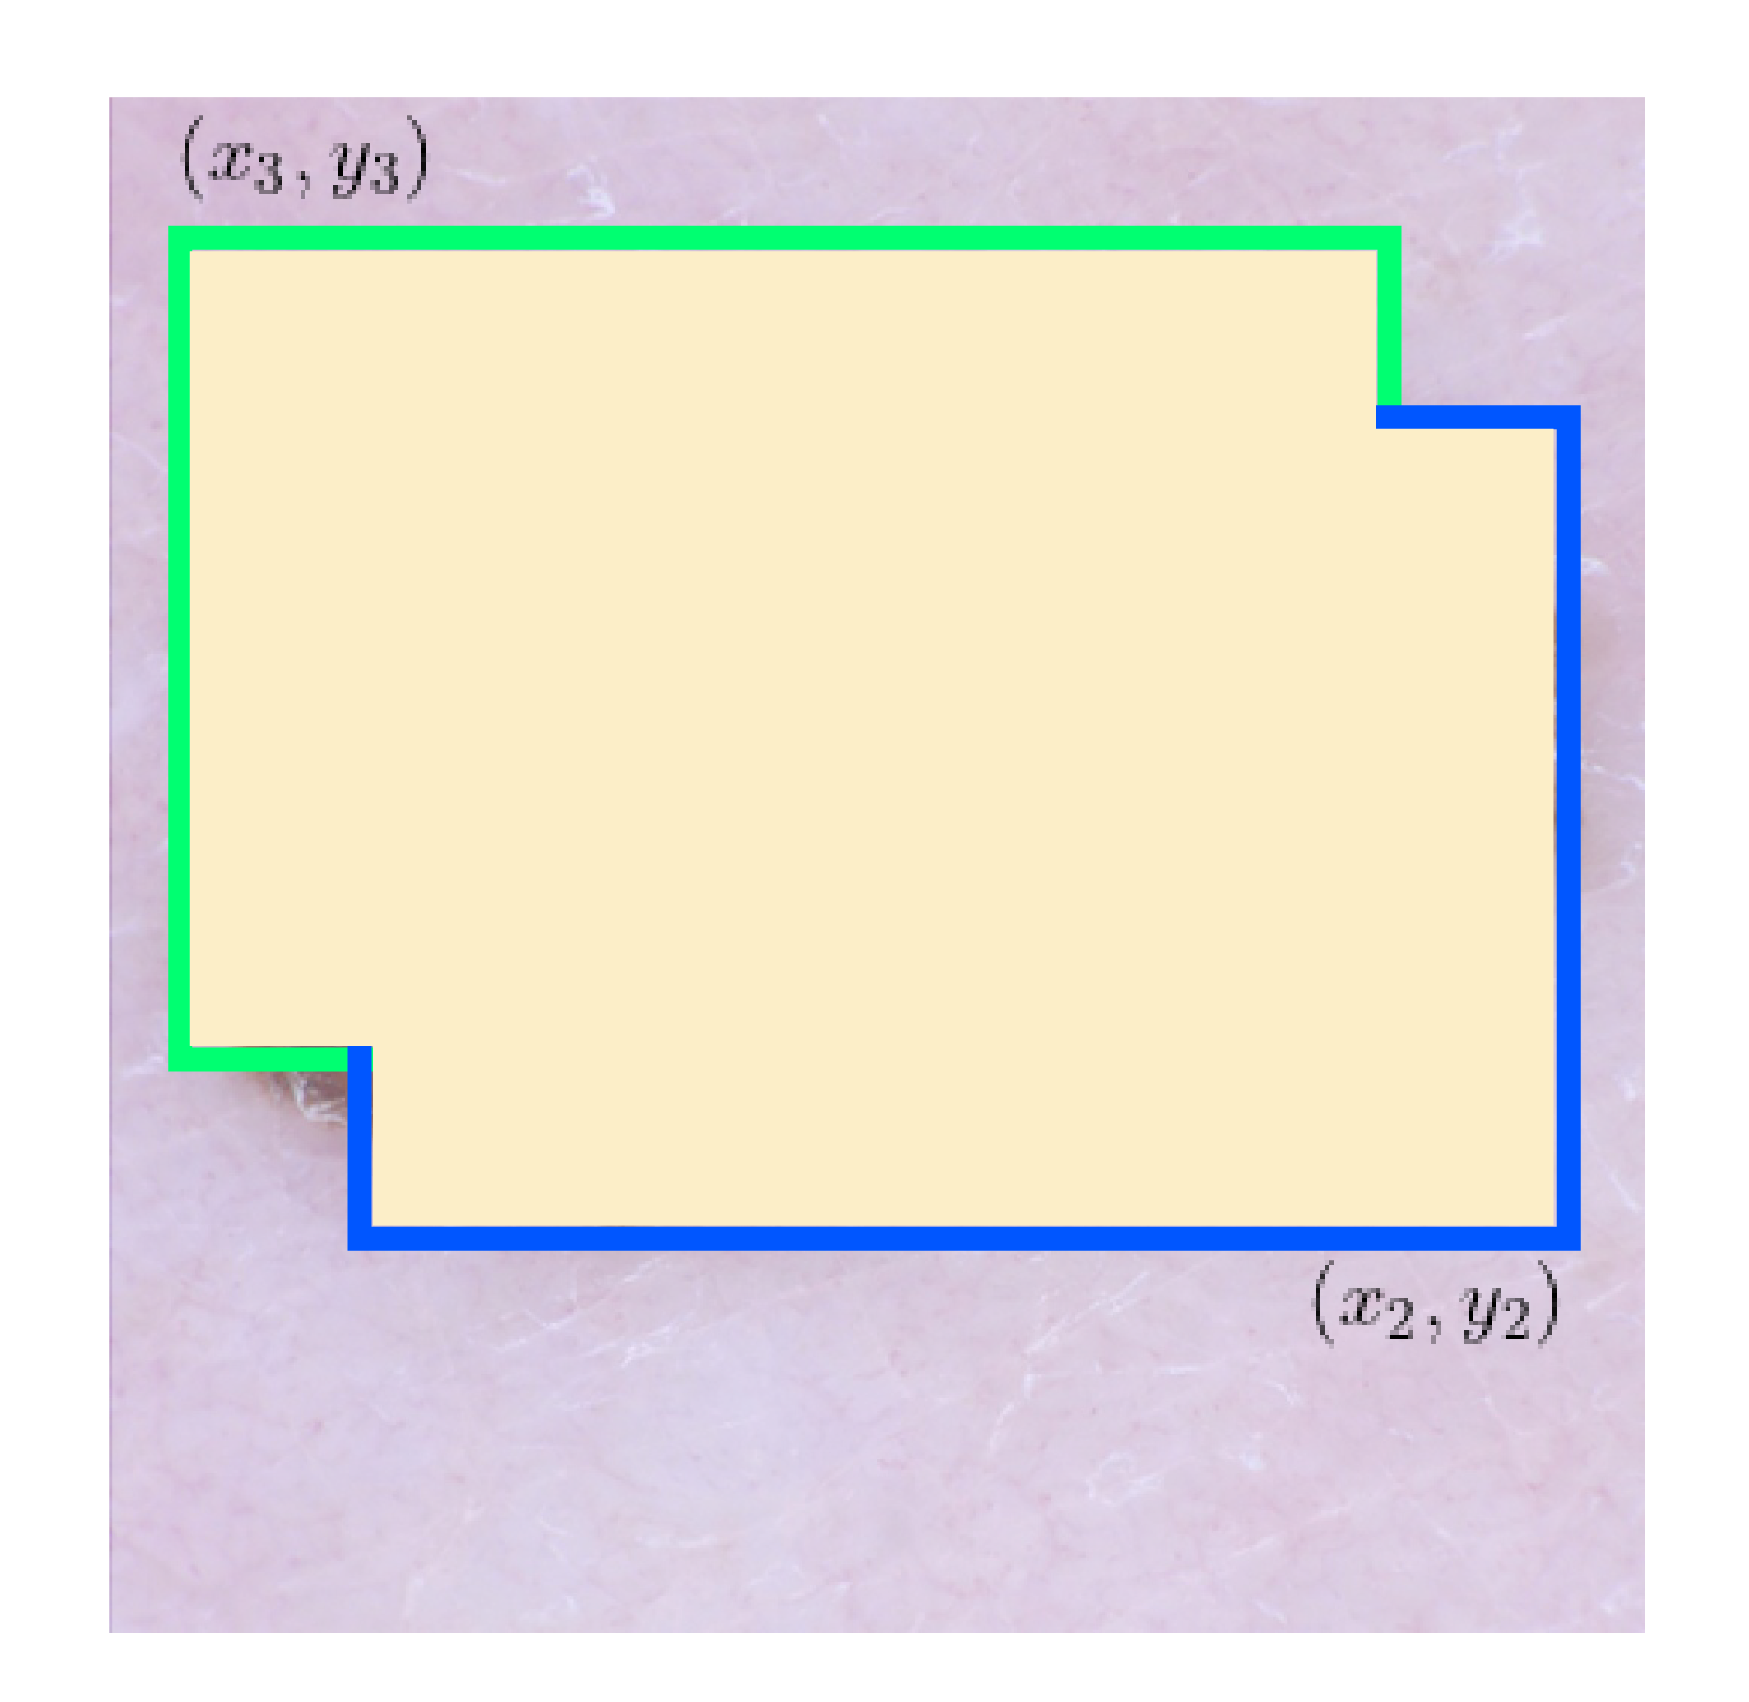
\includegraphics[width=3cm]{../img/bab2/bb-union.png}\\
        (a) &(b) &(c)\\
    \end{tabular}
    \caption{Menunjukkan kondisi kotak pembatas (a) IoU; (b) \textit{Overlap Area} (OA); (c) \textit{Union Area} (UA)}
    \label{fig:iou-cond}
\end{figure}

Dari kedua kotak pembatas tersebut didapatkan dua bagian, yaitu \textit{Overlap Area} (OA) dan \textit{Union Area} (UA). OA merupakan bagian tumpang tindih antara kotak pembatas data aktual dan kotak pembatas hasil prediksi. Sedangkan UA merupakan gabungan antara kedua kotak pembatas. OA dan UA seperti terlihat pada Gambar \ref{fig:iou-cond}. Pembagian antara OA dengan UA menghasilkan nilai IoU seperti pada Persamaan \ref{eq:iou}. Perhitungan OA dan UA seperti terlihat pada Persamaan \ref{eq:oa} dan \ref{eq:ua}. Nilai $x_a1, x_a2, y_a1, y_a2$ pada perhitungan tersebut didapatkan seperti pada Persamaan \ref{eq:xa1} - \ref{eq:ya2}.
\begin{align}
    \label{eq:xa1}
    x_{a1} &= max(x_1, x_3)\\
    \label{eq:ya1}
    y_{a1} &= max(y_1, y_3)\\
    \label{eq:xa2}
    x_{a2} &= min(x_2, x_4)\\
    \label{eq:ya2}
    y_{a2} &= min(y_2, y_4)\\
    \label{eq:oa}
    OA     &= (x_{a2}-x_{a1})\times (y_{a2}-y_{a1})\\
    \label{eq:ua}
    UA     &= (x_2-x_1)\times (y_2-y_1) + (x_4-x_3)\times (y_4-y_3) - OA\\
    \label{eq:iou}
    IoU    &= \frac{OA}{UA}
\end{align}

Dalam menentukan nilai IoU, sangat penting untuk memperhatikan ambang batas IoU. Karena hal ini akan menentukan kategori klasifikasi seperti pada Gambar \ref{fig:iou-cat}. Jika ambang batas IoU adalah $0.5$ maka Gambar \ref{fig:iou-cat} (a) termasuk ke dalam FP, Gambar \ref{fig:iou-cat} (b) dan (c) termasuk ke dalam TP. Sedangkan kondisi kotak pembatas data aktual dan kotak pembatas hasil prediksi tidak beririsan sama sekali dikategorikan sebagai FN.

\begin{figure}[H]
    \centering
    \begin{tabular}{ccc}
        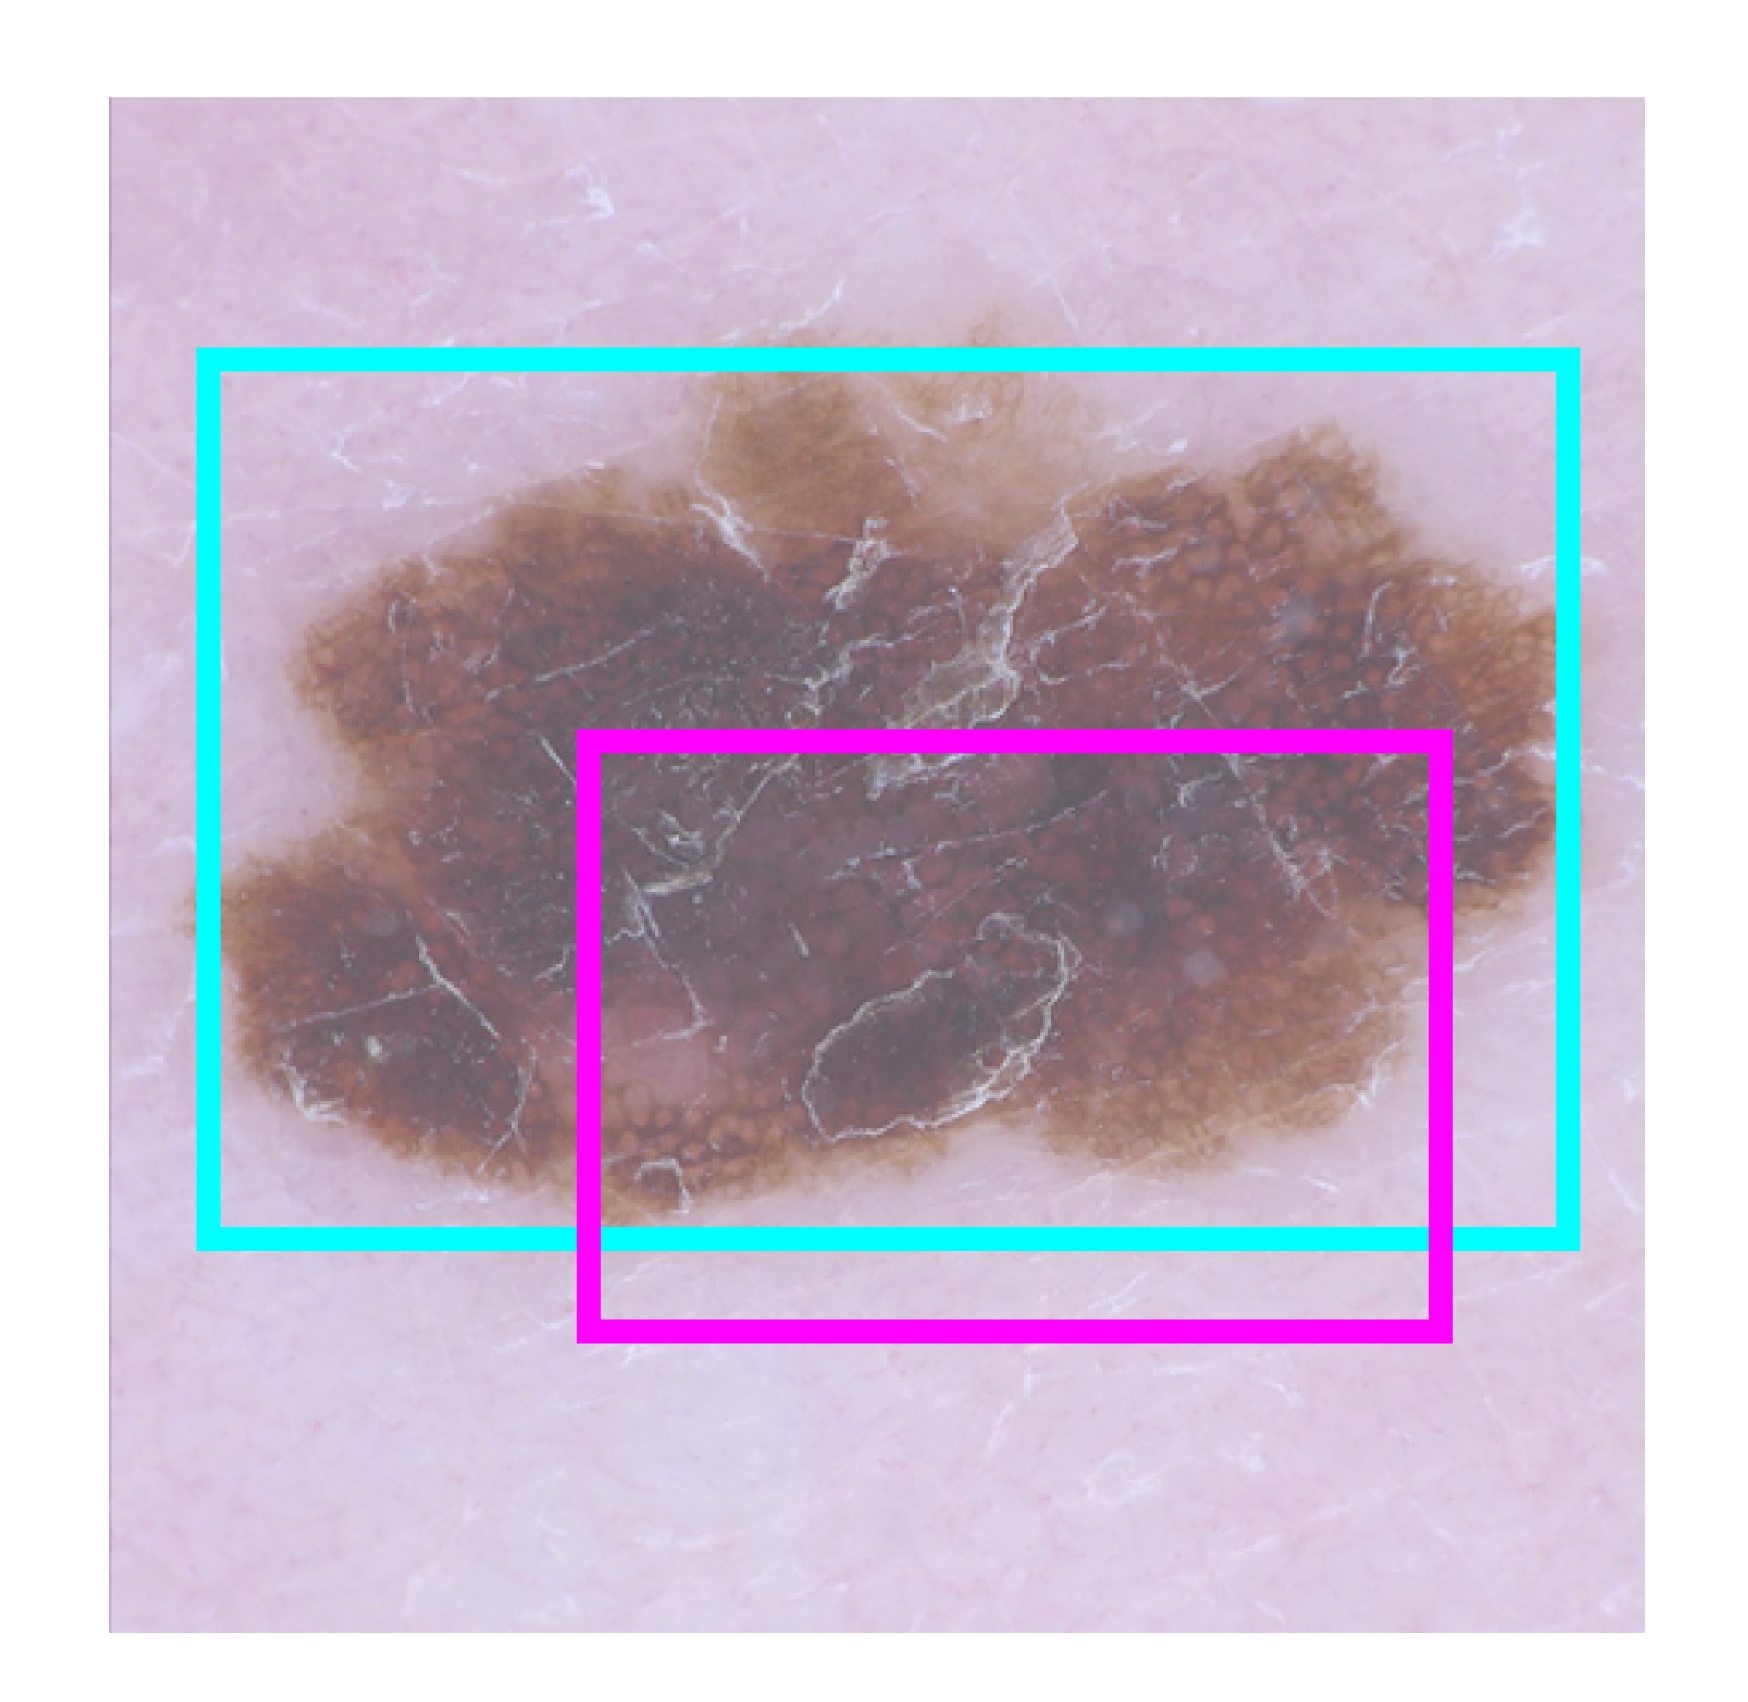
\includegraphics[width=2cm]{../img/bab2/iou-poor.png}
        &
        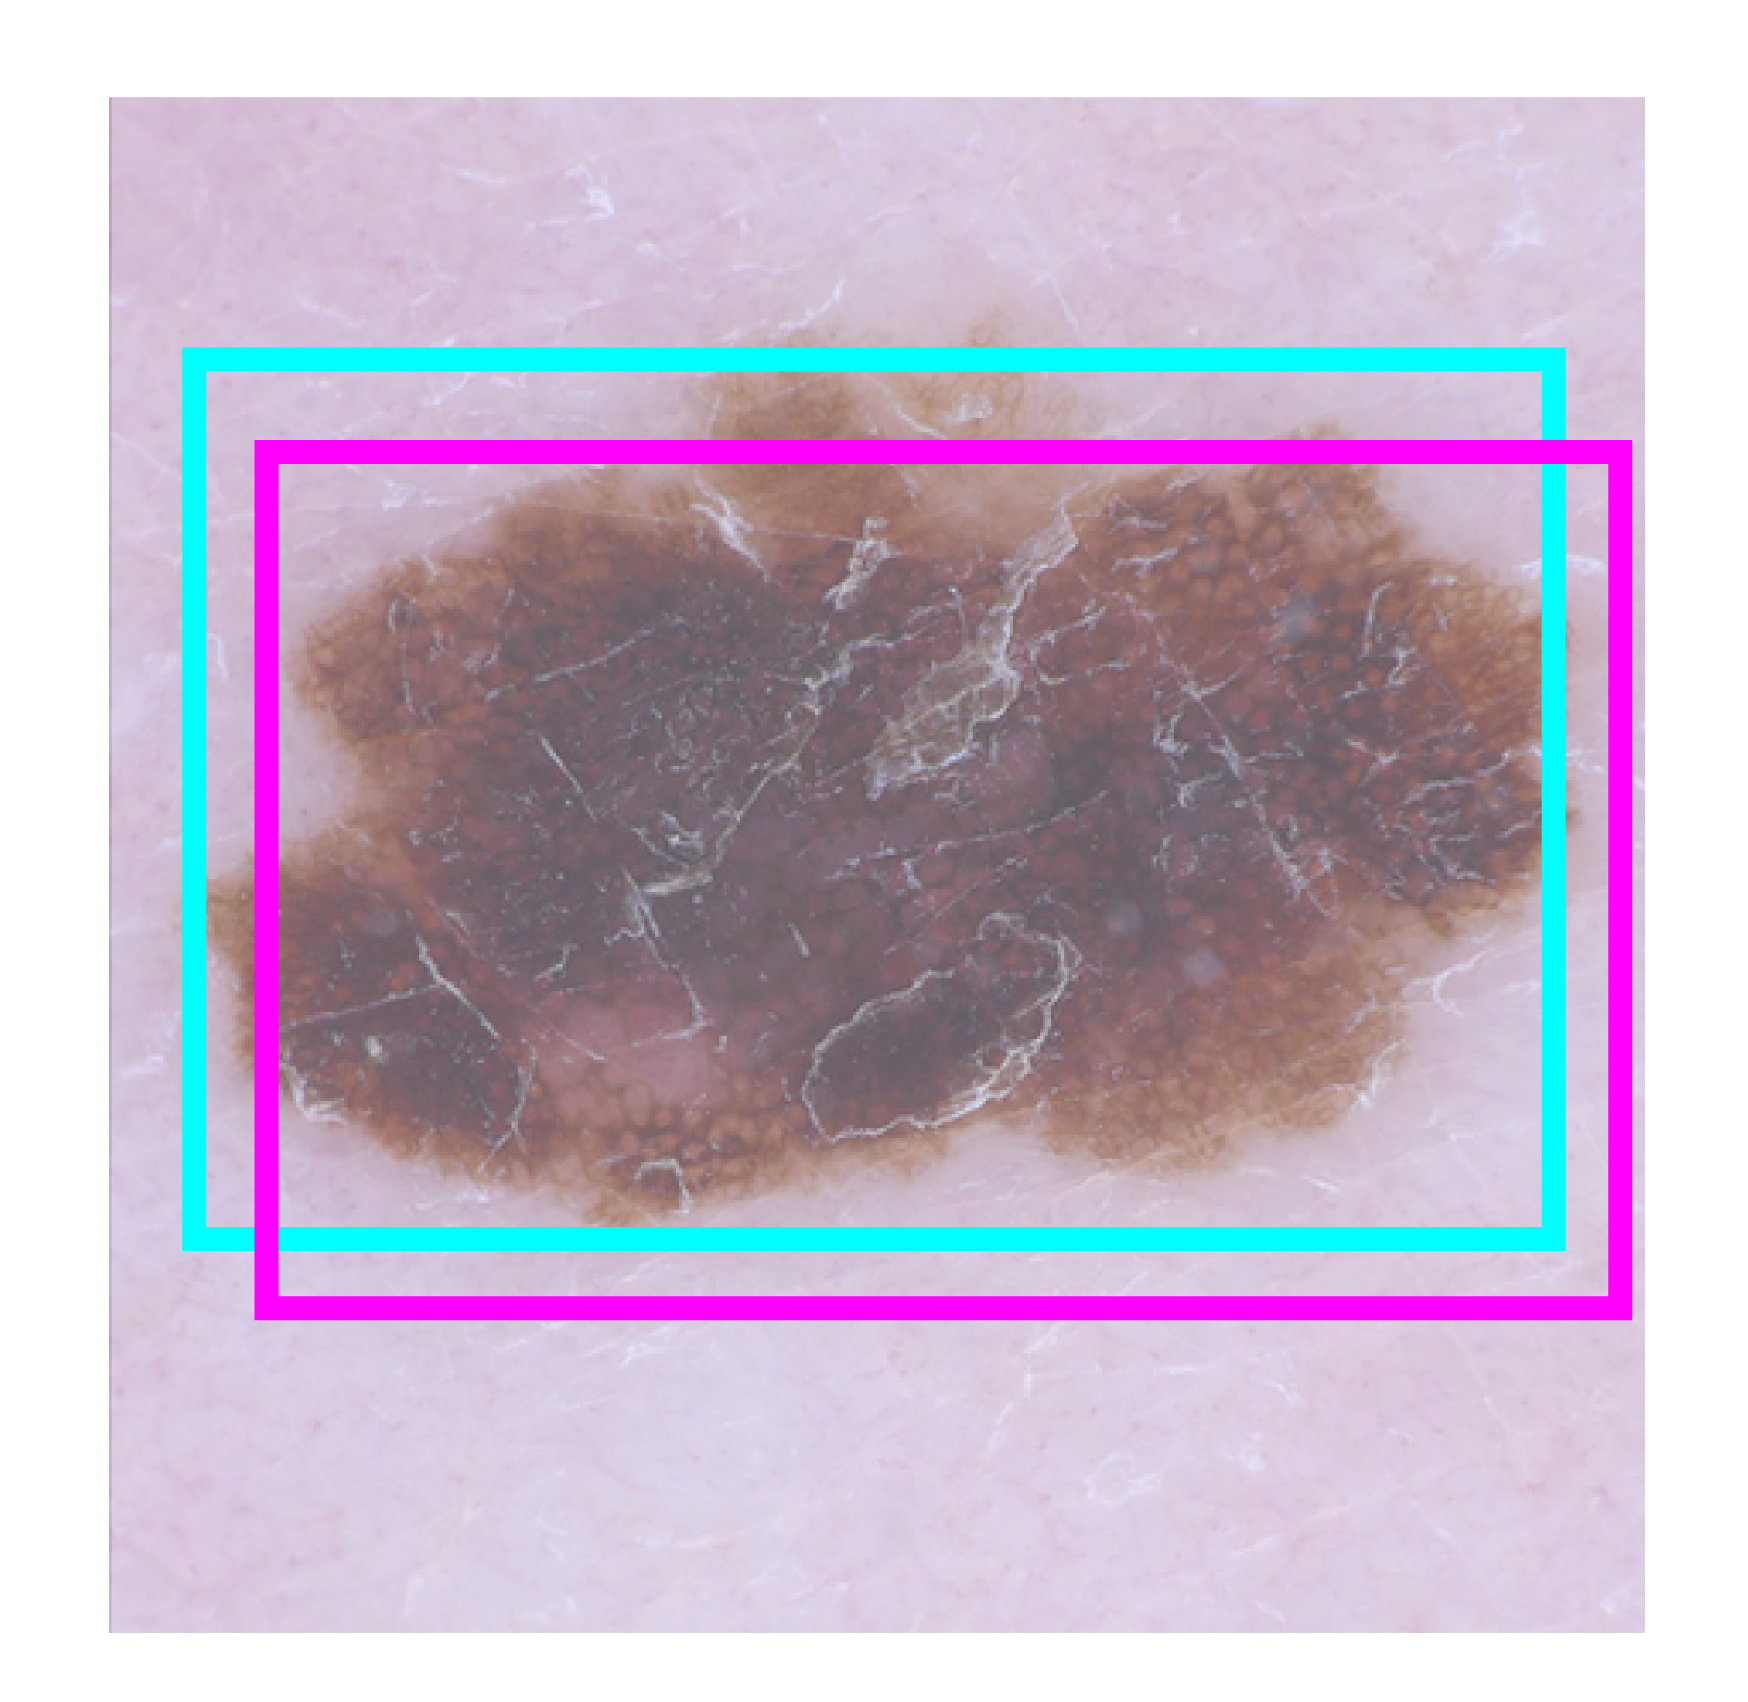
\includegraphics[width=2cm]{../img/bab2/iou-good.png}
        &
        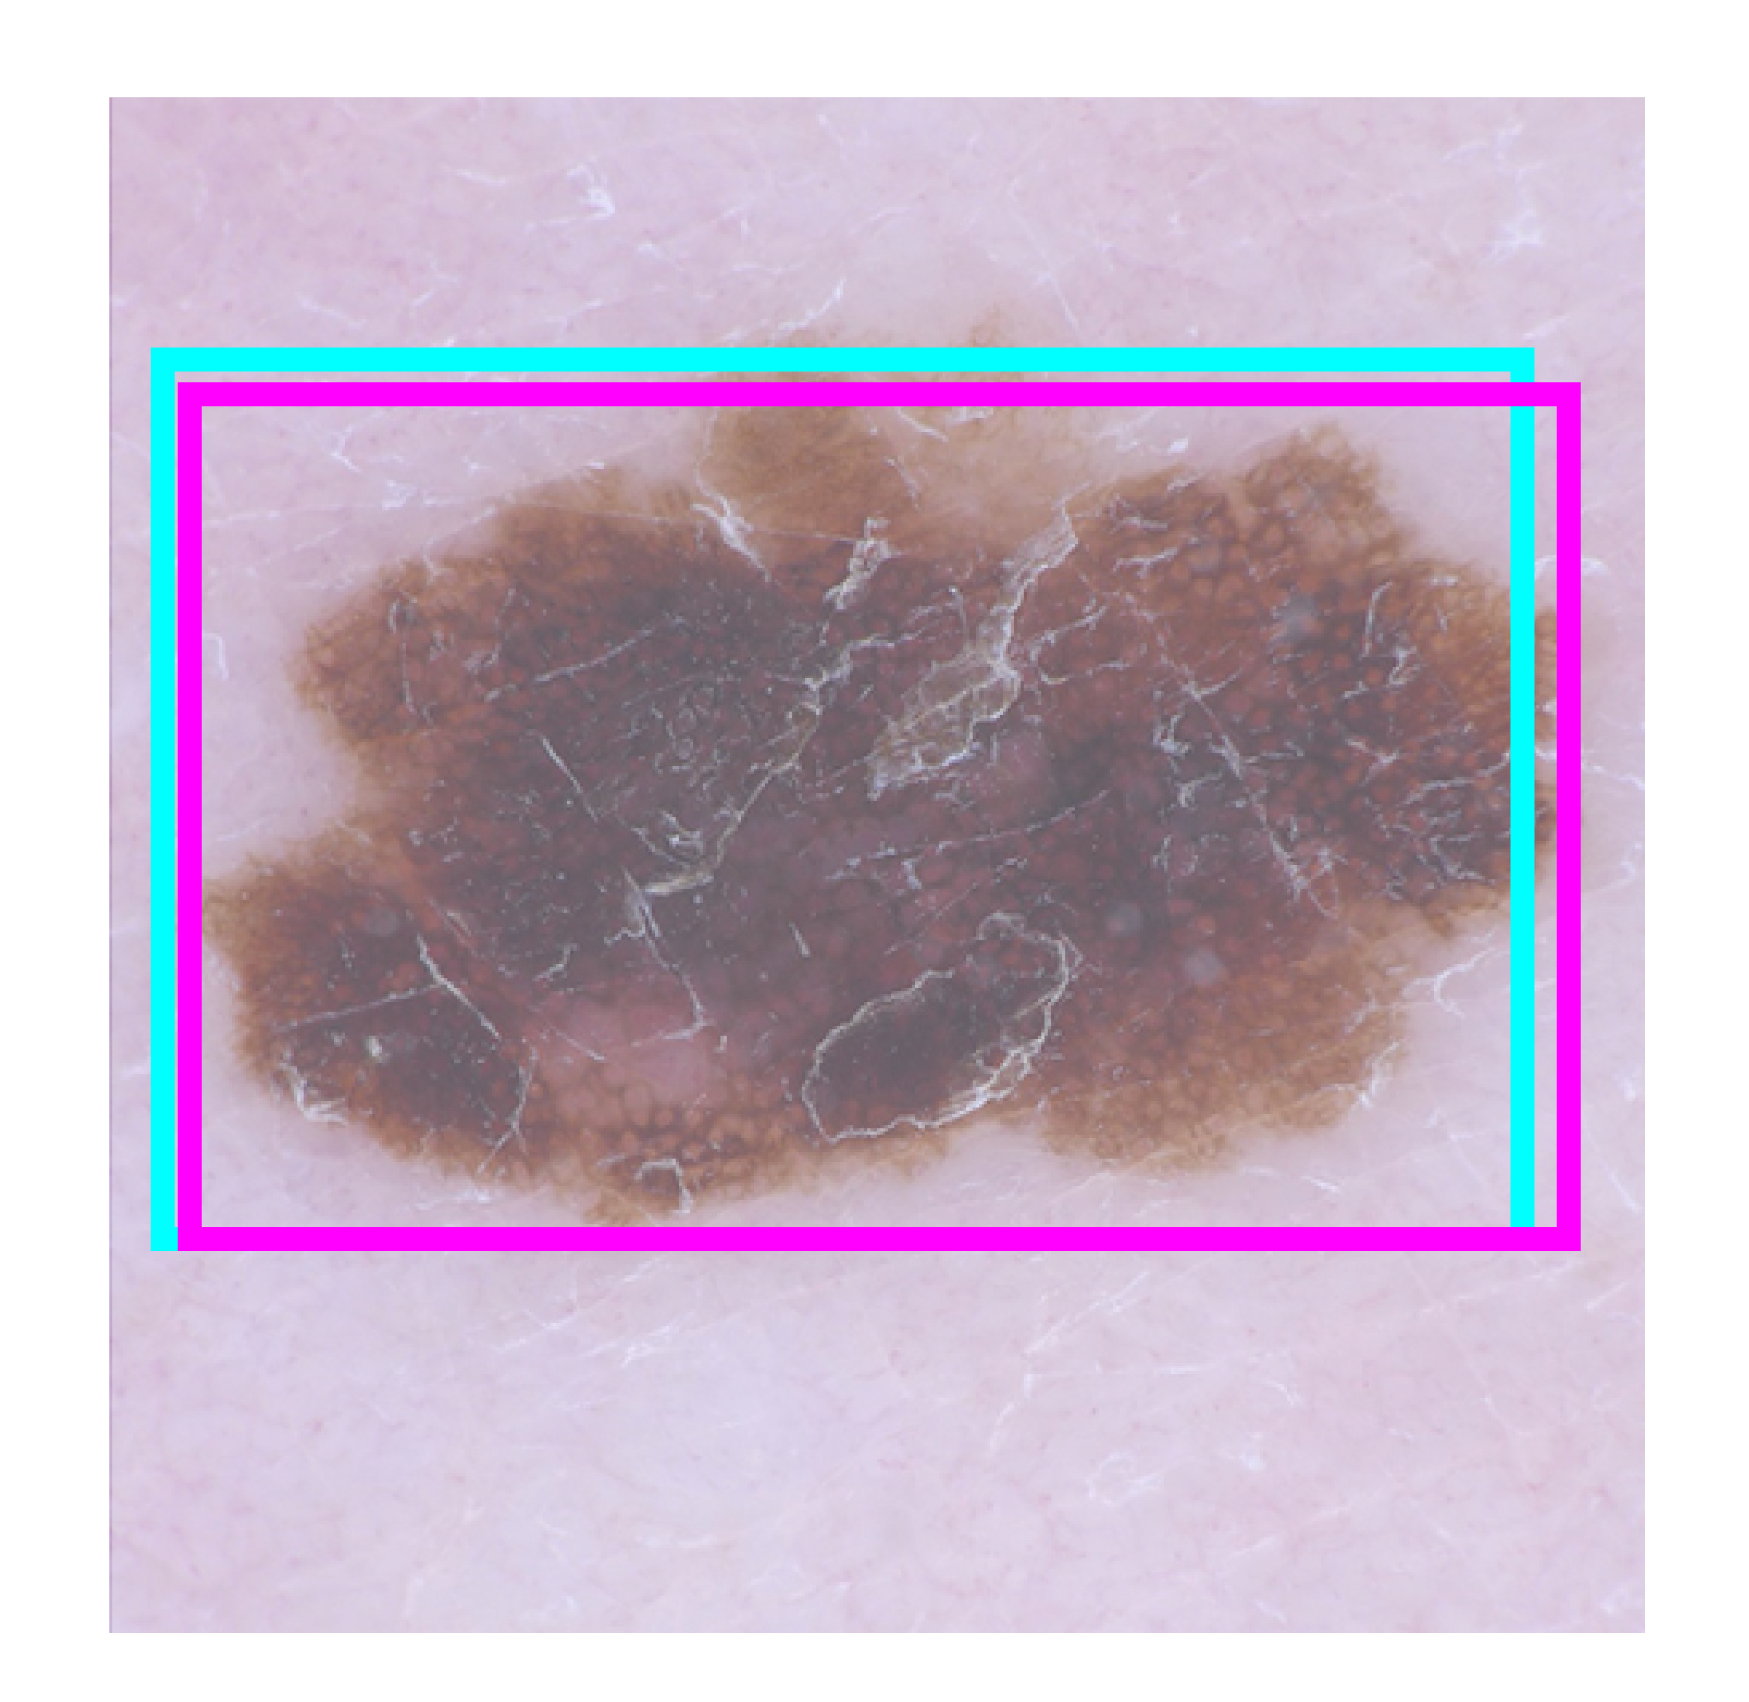
\includegraphics[width=2cm]{../img/bab2/iou-excelent.png}\\
        (a) &(b) &(c)\\
    \end{tabular}
    \caption{Menunjukkan kondisi nilai IoU (a) Nilai IoU kurang baik; (b) Nilai IoU baik; (c) Nilai IoU sangat baik}
    \label{fig:iou-cat}
    Sumber: \citep{Cowton2019}
\end{figure}

\section{\textit{mean Average Precision} (mAP)}
mAP merupakan salah satu metode evaluasi model terutama pada model deteksi objek, seperti Fast R-CNN, MobileNet SSD, dan YOLO. Semakin baik model deteksi objek maka semakin tinggi nilai mAP. mAP menghitung rata-rata \textit{Average Precision} (AP) per kelas seperti terlihat pada Persamaan \ref{eq:map}. AP merupakan perhitungan \textit{precision} dan \textit{recall} pada setiap kelas seperti terlihat pada Persamaan \ref{eq:ap}. Rasio antara kelas positif yang diprediksi dengan benar terhadap seluruh kelas yang diprediksi sebagai positif disebut \textit{precision}. Rasion antara kelas positif yang diprediksi dengan benar terhadap seluruh kelas positif disebut \textit{recall}. Persamaan \ref{eq:precision} dan \ref{eq:recall} menunjukkan perhitungan \textit{precision} dan \textit{recall} dimana $P$ dan $R$ merupakan \textit{precision} dan \textit{recall} \citep{Shultz2017}.
\begin{align}
    \label{eq:precision}
    P &= \frac{TP}{TP+FP}\\
    \label{eq:recall}
    R &= \frac{TP}{TP+FN}\\
    \label{eq:ap}
    AP &= \sum_{i=0}^{n-1} (R_i-R_{i+1})\times P_i\\
    \label{eq:map}
    mAP &= \frac{1}{n}\sum_{i=1}^{n} AP_i
\end{align}

\section{Integrasi Keislaman}
Ujian dari Allah \textit{subhanallahu wa ta'ala} selalu mengiringi kehidupan manusia. Bahkan, awal mula manusia di bumi karena ujian yang diberikan oleh Allah kepada Nabi Adam \textit{'alaihissalam}. Ujian dari Allah \textit{subhanallahu wa ta'ala} dapat berupa perkara yang disukai oleh manusia, seperti harta, tahta, dan wanita. Sedangkan perkara yang tidak disukai oleh manusia, seperti musibah, penyakit, dan kesengsaraan. Musibah dapat berupa bencana seperti musim paceklik yang akan menimpa suatu kaum pada masa Nabi Yusuf \textit{'alaihissalam} sebagaimana dalam firman-Nya:

\begin{flushright}
    \begin{RLtext}
        قَالَ تَزْرَعُوْنَ سَبْعَ سِنِيْنَ دَاَبًاۚ فَمَا حَصَدْتُّمْ فَذَرُوْهُ فِيْ سُنْۢبُلِهٖٓ اِلَّا قَلِيْلًا مِّمَّا تَأْكُلُوْنَ (٧٤) ثُمَّ يَأْتِيْ مِنْۢ بَعْدِ ذٰلِكَ سَبْعٌ شِدَادٌ يَّأْكُلْنَ مَا قَدَّمْتُمْ لَهُنَّ اِلَّا قَلِيْلًا مِّمَّا تُحْصِنُوْنَ (٨٤)
    \end{RLtext}
\end{flushright}

Artinya: "(Yusuf) berkata, 'Bercocoktanamlah kamu tujuh tahun berturut-turut! Kemudian apa yang kamu tuai, biarkanlah di tangkainya, kecuali sedikit untuk kamu makan. Kemudian, sesudah itu akan datang tujuh (tahun) yang sangat sulit (paceklik) yang menghabiskan apa yang kamu simpan untuk menghadapinya, kecuali sedikit dari apa (bibit gandum) yang kamu simpan." (Yusuf: 47-48). Sebagaimana yang dikabarkan Nabi Yusuf \textit{'alaihissalam} dalam ayat tersebut bahwa akan terdapat musim paceklik selama tujuh tahun. Pada musim tersebut tidak akan ada tumbuhan yang dapat hidup dan seluruh hasil panen akan gagal. Oleh sebab itu, Nabi Yusuf \textit{'alaihissalam} berkata kepada mereka, "... yang menghabiskan apa yang kalian simpan untuk menghidupinya (tahun sulit), kecuali sedikit dari (bibit gandum) yang kalian simpan". Imam Ibnu Katsir menafsirkan ayat ini dengan menjelaskan bahwa seseorang harus melakukan persiapan sebelum bencana terjadi sebagaimana penyakit yang akan menimpa. Jika muncul suatu kecurigaan atau muncul suatu pertanda dari penyakit dianjurkan untuk melakukan upaya pencegahan \citep{Katsir2015}.
% TODO: Tambahkan sitasi imam ibnu katsir

    \subsection{Hikmah Orang Sakit}
    Seorang mukmin tidak akan pernah terlepas dari tiga keadaan, yaitu jika mendapat nikmat maka ia bersyukur, jika mendapat susah maka ia bersabar, dan jika membuat dosa maka ia bertaubat. Hal ini merupakan kebahagiaan bagi seorang mukmin sebagaimana sabda Rasulullah \textit{shalallahu 'alaihi wa sallam}, 
    
    \begin{flushright}
        \begin{RLtext}
            عَجَبًا ِلأَمْرِ الْمُؤْمِنِ إنَّ أَمْرَهُ كُلَّهُ لَهُ خَيْرٌ وَلَيْسَ ذَلِكَ ِلأَحَدٍ إِلاَّ لْمُؤْمِنِ، إِنْ أَصَابَتْهُ سَرَّاءُ شَكَرَ فَكَانَ خَيْرًا لَهُ، وَإِنْ أَصَابَتْهُ ضَرَّاءُ صَبَرَ فَكَانَ خَيْراً لَهُ
        \end{RLtext}
    \end{flushright}

    Artinya: "Sungguh menakjubkan perkara seorang mukmin, sesungguhnya semua urusannya merupakan kebaikan, dan hal ini tidak terjadi kecuali bagi orang mukmin. Jika dia mendapat kegembiraan, maka dia bersyukur dan itu merupakan kebaikan baginya, dan jika mendapat kesusahan, maka dia bersabar dan ini merupakan kebaikan baginya." (HR. Muslim: 2999). Ketika seseorang mendapatkan nikmat dan bersyukur maka akan mendapatkan kebaikan dari Allah \textit{azza wa jalla}. Ketika seseorang mendapat kesusahan dan bersabar maka akan mendapatkan kebaikan pula dari Allah \textit{azza wa jalla}.

    Penyakit merupakan salah satu jalan untuk mendapatkan ampunan dosa dari Allah \textit{subhanallahu wa ta'ala}. Namun, terdapat ketentuan untuk mendapatkan pengampunan dosa ketika sakit, seperti tidak menjalankan maksiat ketika sakit atau tetap dalam ketakwaan ketika sakit. Rasulullah \textit{shalallahu 'alaihi wa sallam} bersabda, "Tidaklah menimpa seorang mukmin rasa sakit yang terus menerus, kepayahan, penyakit, dan juga kesedihan, bahkan sampai kesusahan yang menyusahkannya, melainkan akan dihapuskan dengannya dosa-dosanya." (HR. Muslim). Di sisi lain, penyakit juga merupakan peringatan dan hukuman dari apa yang telah diperbuat sebagaimana firman Allah \textit{subhanallahu wa ta'ala} dalam surat asy-Syura ayat 30,

    \begin{flushright}
        \<وَمَآ اَصَابَكُمْ مِّنْ مُّصِيْبَةٍ فَبِمَا كَسَبَتْ اَيْدِيْكُمْ وَيَعْفُوْا عَنْ كَثِيْرٍۗ (٠٣)>
    \end{flushright}

    Artinya: "Dan apa saja musibah yang menimpamu maka adalah disebabkan oleh perbuatan tanganmu sendiri, dan Allah memaafkan sebagian besar (dari kesalahan-kesalahanmu)." (asy-Syura: 30).

    \subsection{Ikhtiar Orang Sakit}
    Tiap-tiap orang yang sakit pasti menginginkan kesembuhan. Bagi orang sakit, usaha untuk sembuh merupakan keharusan karena dapat mengganggu ketakwaan kepada Allah \textit{subhanallahu wa ta'ala} jika sakit tidak segera dihilangkan. Syaikh Muhammad bin Shalih al-'Utsaimin \textit{rahimahullah} mengatakan bahwa ikhtiar untuk mendapatkan kesembuhan bagi orang sakit adalah suatu keharusan karena jika ditinggalkan dapat membahayakan tubuh. Hal ini mempertimbangkan fungsionalitas tubuh sebagai sarana beribadah kepada Allah \textit{subhanallahu wa ta'ala}. Misalnya, perlunya usaha untuk menghilangkan kanker pada seseorang yang terkena penyakit kanker. Kanker akan menyebar lebih luas ke jaringan tubuh lain dan memunculkan penyakit baru jika tidak segera ditangani. Oleh karena itu, menghilangkan kanker yang membahayakan merupakan suatu keharusan bagi seorang mukmin. Upaya untuk mencari kesembuhan dan tidak berputus asa dari penyakit telah diperintahkan oleh rasulullah \textit{shalallahu 'alaihi wa sallam}. Dari Jabir bin 'Abdillah, Rasulullah \textit{shalallahu 'alaihi wa sallam} bersabda,

    \begin{flushright}
        \<لِكُلِّ دَاءٍ دَوَاءٌ فَإِذَا أُصِيبَ دَوَاءُ الدَّاءِ بَرَأَ بِإِذْنِ اللَّهِ عَزَّ وَجَلَّ>
    \end{flushright}

    Artinya: “Setiap penyakit itu pasti ada obatnya. Oleh karena itu, barang siapa yang tepat dalam melakukan pengobatan suatu penyakit, maka dengan izin Allah ‘azza wa  jalla dia akan sembuh.” (HR. Muslim, Ibn Hiban, dan Hakim). Dari Abu Hurairah \textit{radhiallahu 'anhu}, dia mengabarkan bahwa Rasulullah \textit{shalallahu 'alaihi wa sallam} bersabda,

    \begin{flushright}
        \<ما أنْزَلَ اللَّهُ داءً إلَّا أنْزَلَ له شِفاءً>
    \end{flushright}

    “Tidaklah Allah menurunkan suatu penyakit, melainkan Dia turunkan obat untuknya.” (HR. Ibn Majah dan dishahihkan al-Albani).

    Berdasarkan sifat kanker kulit yang dapat menyebar ke jaringan di sekitarnya, kanker kulit termasuk ke dalam penyakit yang harus segera ditangani. Bahkan, deteksi kanker kulit yang membahayakan sangat diperlukan untuk mendiagnosis kanker kulit yang berbahaya dan tidak berbahaya. Salah satu usaha untuk mendapatkan kesembuhan dari kanker kulit adalah melakukan diagnosis kanker kulit. Penelitian ini melakukan diagnosis kanker kulit dengan metode YOLO-v7 untuk mengetahui jenis kanker kulit yang diderita sehingga dapat meminimalisir resiko yang terjadi akibat kanker kulit.









    \chapter{METODE PENELITIAN}

\section{Jenis Penelitian}
Penelitian ini melakukan deteksi objek pada data citra dermoskopi menggunakan metode YOLO-v7. Berdasarkan hal tersebut, penelitian ini data numerik yang terdiri dari matriks dan nilai intensitas piksel sehingga penelitian ini termasuk ke dalam penelitian kuantitatif. Maka dari itu, pada penelitian ini terdapat perhitungan dan analisis terkait dengan data dan metode yang digunakan untuk mendeteksi kanker kulit pada citra dermoskopi.

\section{Jenis dan Sumber Data}
Penelitian ini menggunakan dataset yang berasal dari \textit{ISIC 2019 Challenge}. Dataset \textit{ISIC 2019 Challenge} memiliki 8 jenis kanker kulit, yaitu \textit{Actinic Keratosis}, \textit{Melanoma}, \textit{Squamous Cell Carcinoma}, \textit{Basal Cell Carcinoma}, \textit{Nevus}, \textit{Dermatofibroma}, \textit{Benign Keratosis Lesion}, dan \textit{Vascular Lesion}. Terdapat ribuan data citra kanker kulit, akan tetapi dengan mempertimbangkan perangkat yang digunakan untuk pembentukan model, penelitian ini menggunakan 200 citra pada tiap kelas sehingga terdapat 1600 data citra yang digunakan pada penelitian ini untuk pembentukan model. Sampel citra masing-masing jenis kanker kulit seperti terlihat pada Gambar \ref{fig:dataset}.

\begin{figure}[H]
    \centering
    \begin{tabular}{cccc}
        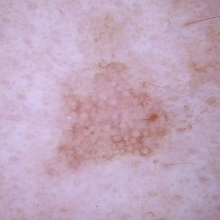
\includegraphics[width=2cm]{../img/Dataset - AK.png}
        &
        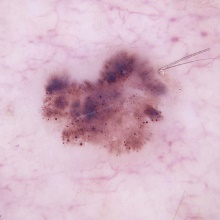
\includegraphics[width=2cm]{../img/Dataset - BCC.png}
        &
        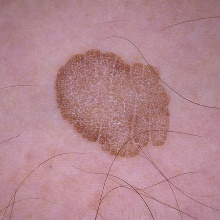
\includegraphics[width=2cm]{../img/Dataset - BKL.png}
        &
        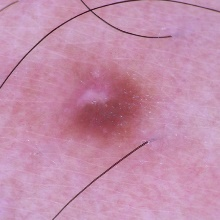
\includegraphics[width=2cm]{../img/Dataset - DF.png}\\
        (a) &(b) &(c) &(d)\\
        \  &\  &\  &\ \\
        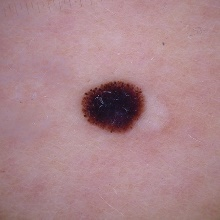
\includegraphics[width=2cm]{../img/Dataset - MEL.png}
        &
        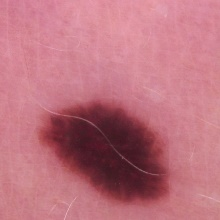
\includegraphics[width=2cm]{../img/Dataset - NV.png}
        &
        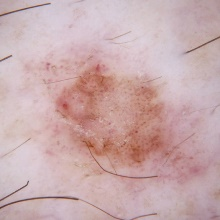
\includegraphics[width=2cm]{../img/Dataset - SCC.png}
        &
        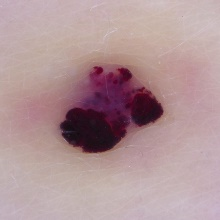
\includegraphics[width=2cm]{../img/Dataset - VASC.png}\\
        (e) &(f) &(g) &(h)\\
    \end{tabular}
    \caption{Dataset citra dermoskopi kanker kulit (a) AK; (b) BCC; (c) BKL; (d) DF; (e) MEL; (f) NV; (g) SCC; (h) VASC;}
    \label{fig:dataset}
\end{figure}

\section{Kerangka Penelitian}
Tahapan dalam melakukan deteksi kanker kulit berdasarkan citra dermoskopi menggunakan YOLO-v7 pada penelitian ini seperti terlihat pada Gambar \ref{fig:flowchart}.

\begin{figure}[H]
    \begin{center}
        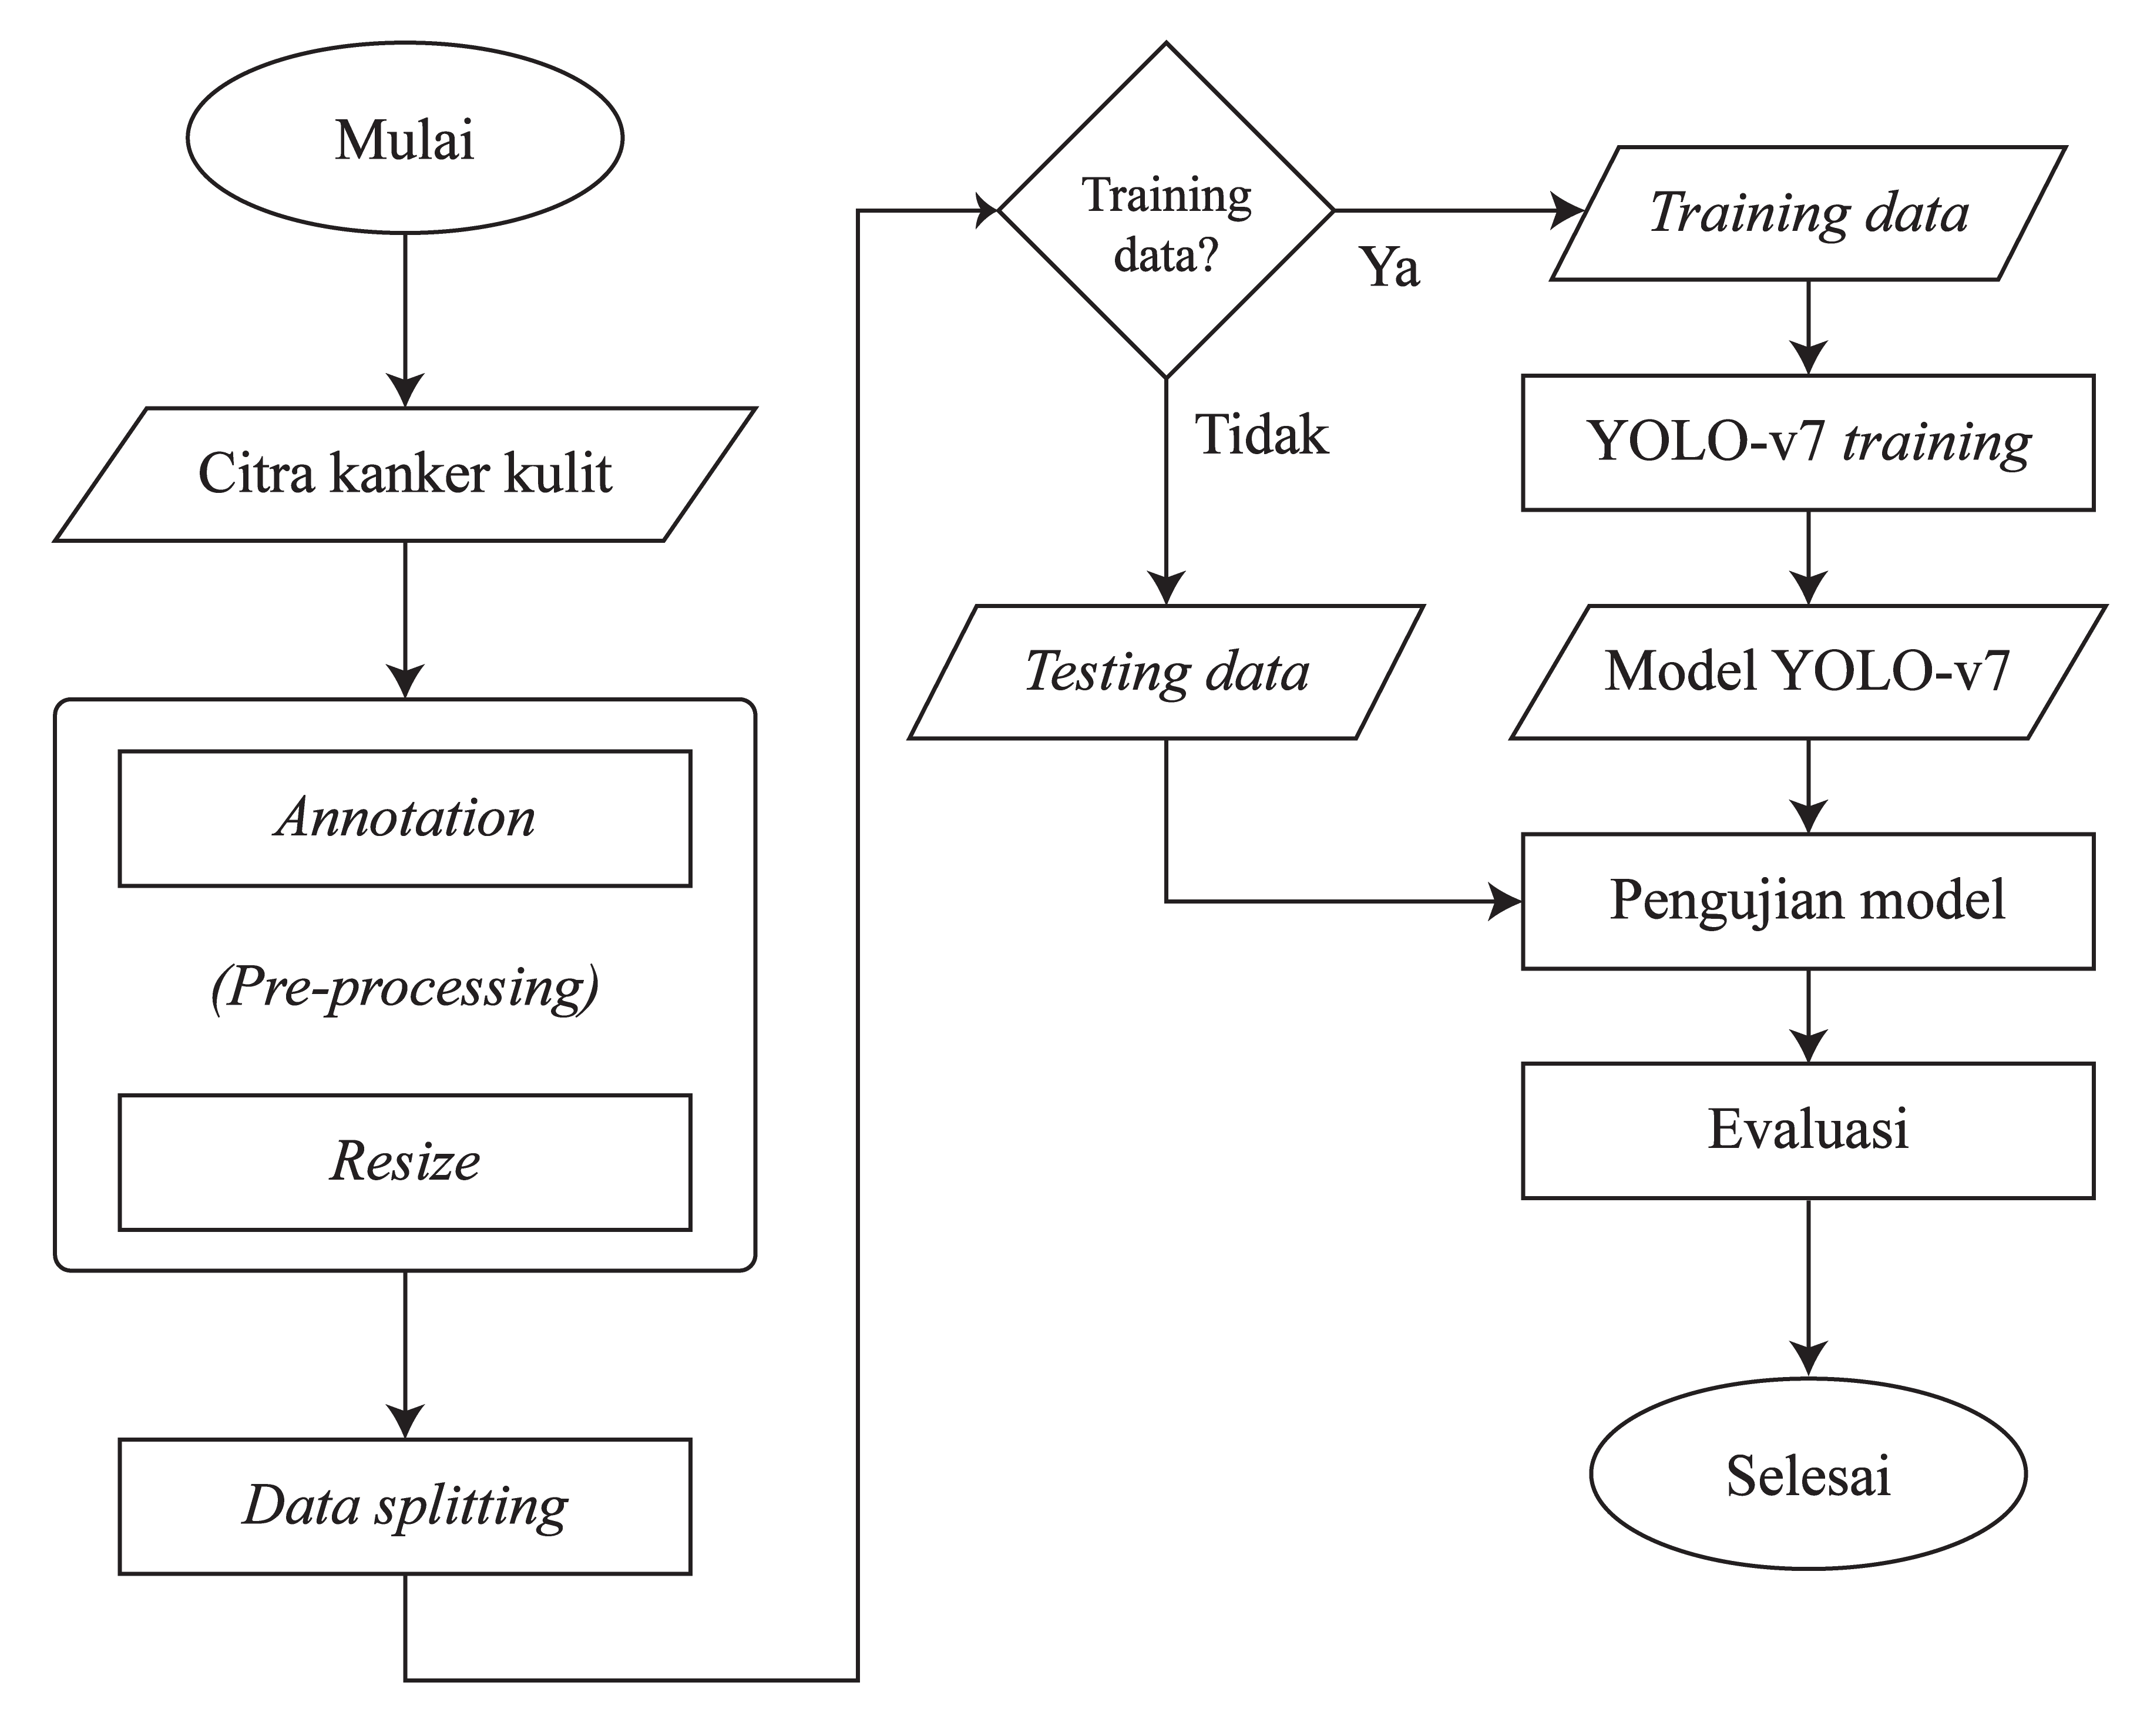
\includegraphics[width=13cm]{../img/Flowchart.png}
        \caption{Diagram alir pada penelitian ini}
        \label{fig:flowchart}
    \end{center}
\end{figure}

Penelitian ini terdiri dari beberapa proses sebagai berikut:
\begin{enumerate}
    \item Tahap \textit{pre-processing} terdiri dari \textit{annotation} dan \textit{resize}. \textit{Annotation} merupakan pemberian kotak pembatas sebuah objek pada sebuah citra. Hal ini dilakukan satu per satu sesuai dengan label yang diberikan dari penyedia dataset, yaitu \textit{ISIC 2019 Challenge}. \textit{Resize} merupakan pengubahan ukuran piksel pada sebuah citra, sehingga penelitian ini melakukan \textit{resize} citra masukan menjadi ukuran $640\times 640$. Rumus \textit{resize} seperti terlihat pada \ref{eq:resize}. Proses \textit{annotation} dan \textit{resize} seperti terlihat pada Gambar \ref{fig:preprocessing}.
    \begin{figure}[H]
        \centering
        \begin{tabular}{ccc}
            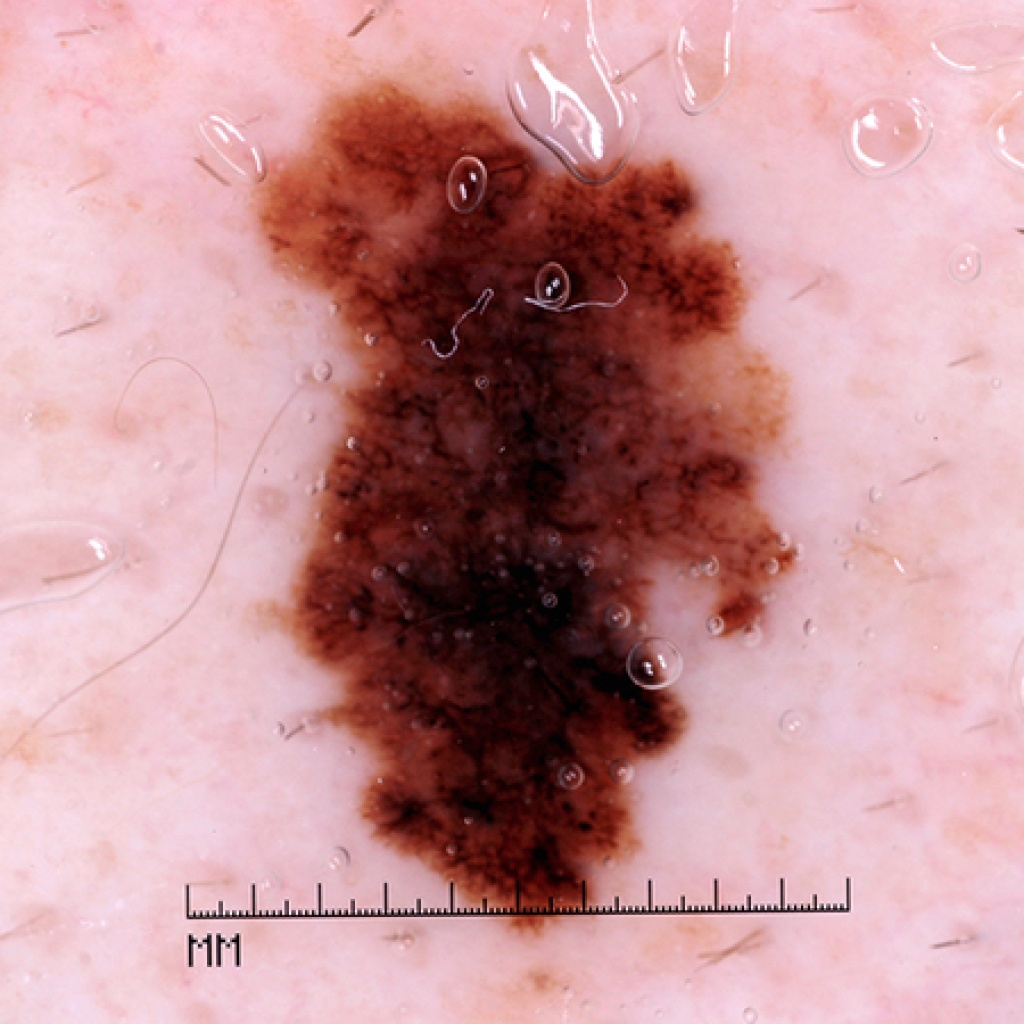
\includegraphics[width=2cm]{../img/bab2/dermoscopy.jpg}
            &
            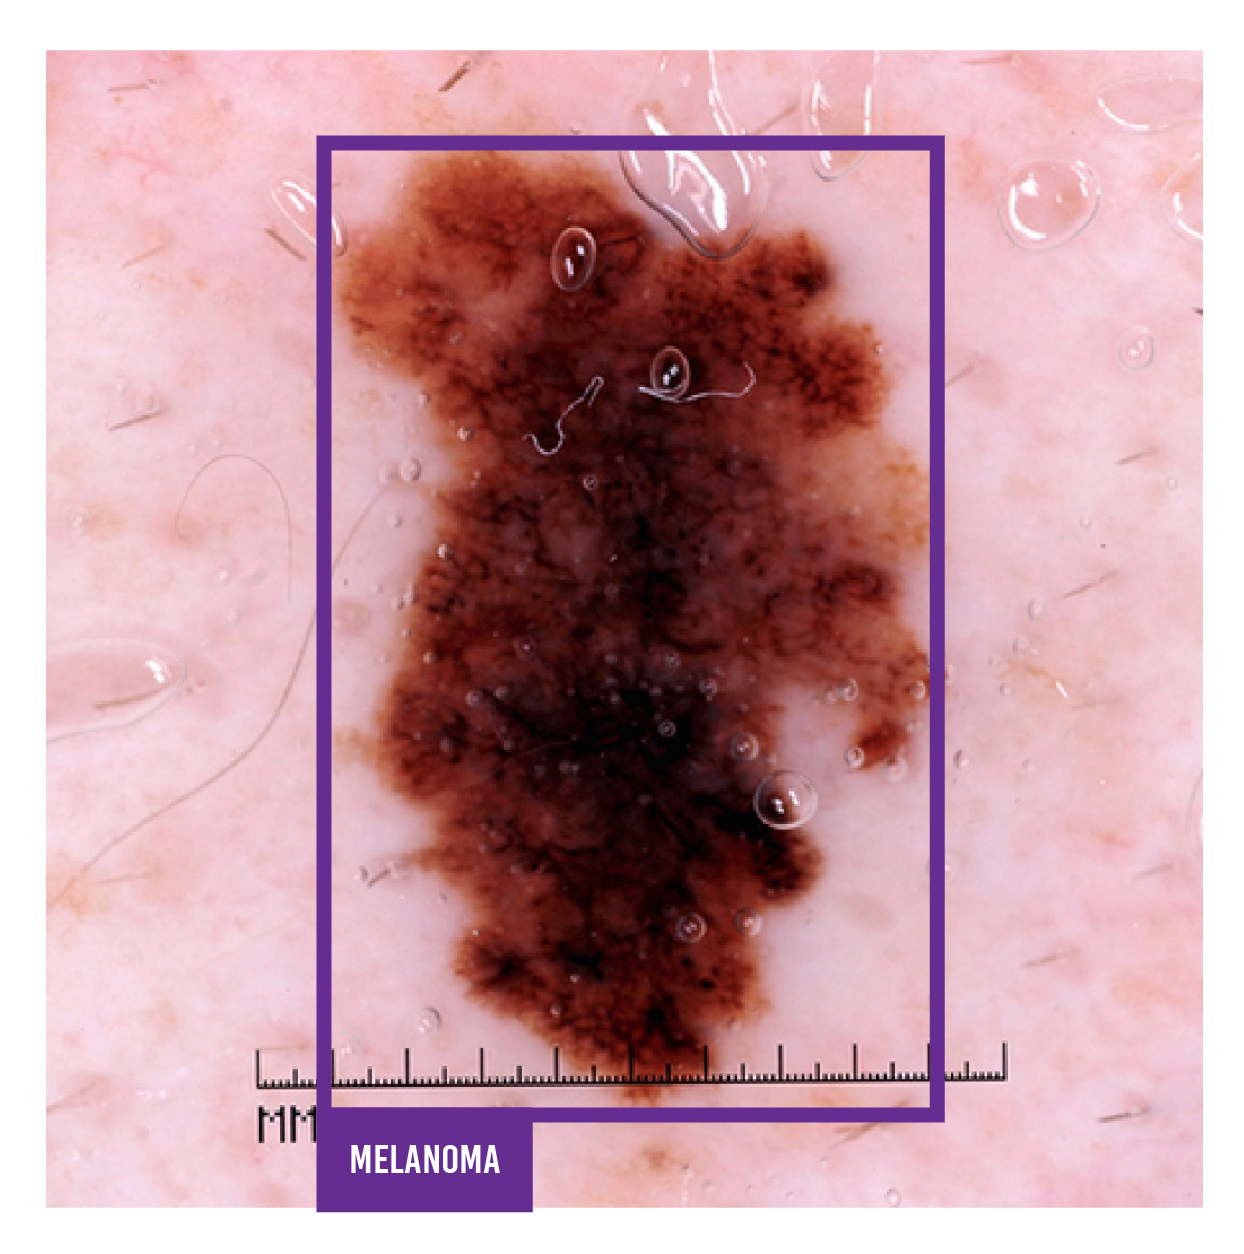
\includegraphics[width=2cm]{../img/Annotation - Latex.png}
            &
            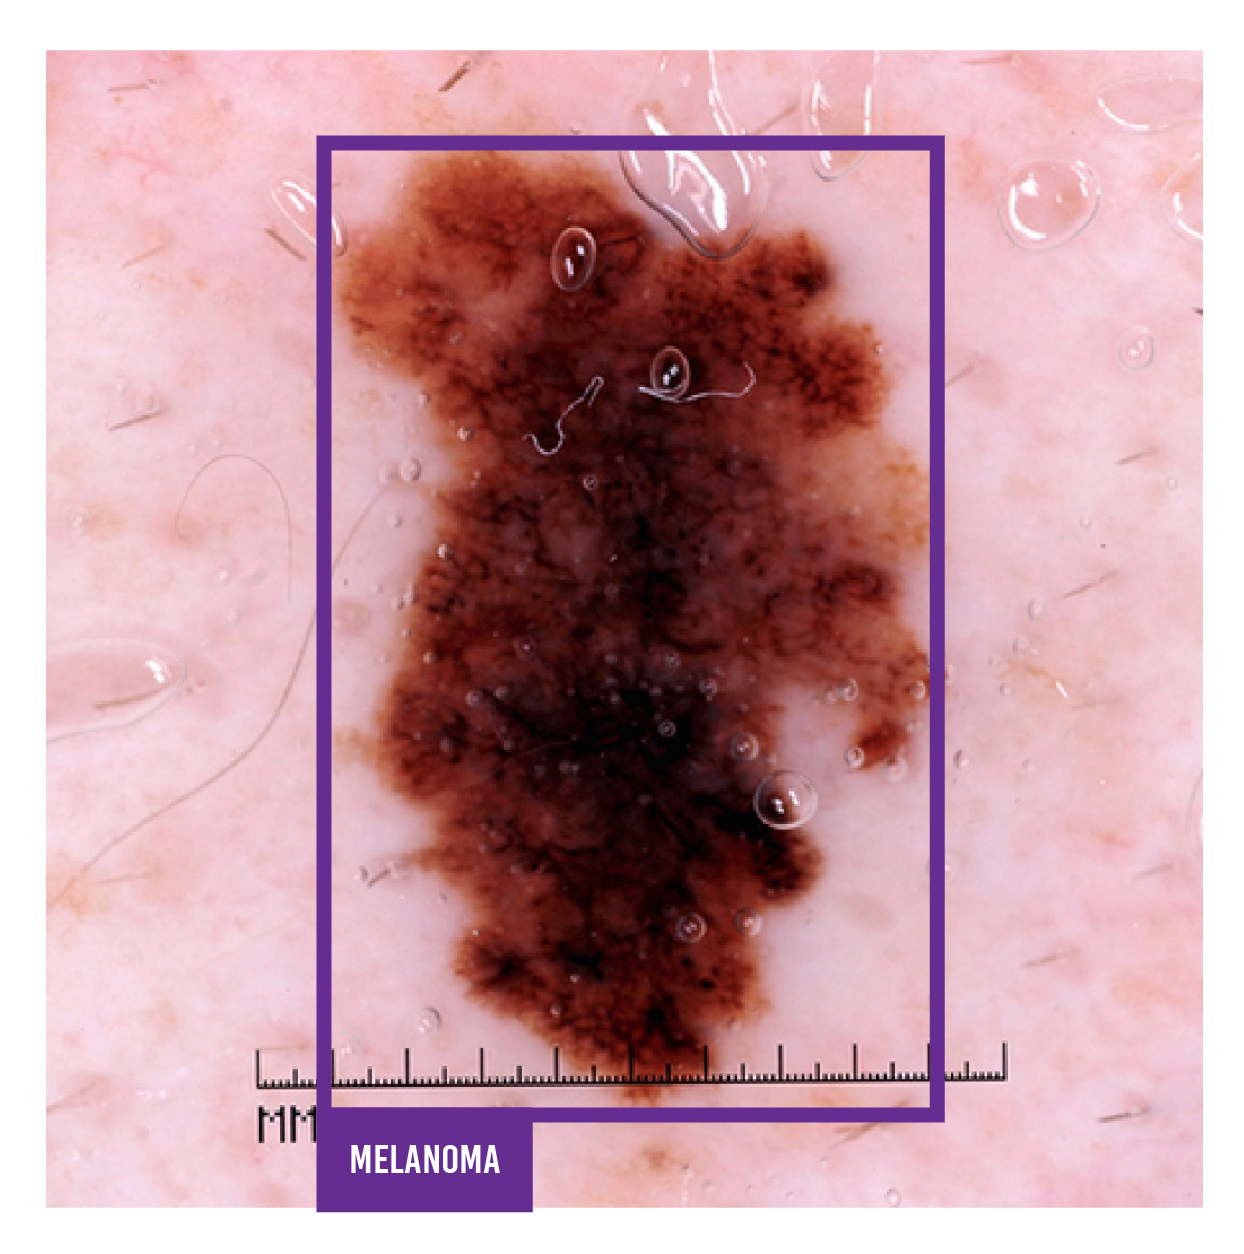
\includegraphics[width=1.5cm]{../img/Annotation - Latex.png}\\
            (a) &(b) &(c)\\
        \end{tabular}
        \caption{Tahap \textit{pre-processing} (a) Citra asli; (b) Citra setelah menerapkan \textit{annotation}; (c) Citra setelah menerapkan \textit{resize}}
        \label{fig:preprocessing}
    \end{figure}

    \item \textit{Data splitting} merupakan tahap pembagian data. Penelitian ini membagi data menjadi tiga, yaitu $70\%$ data untuk proses pelatihan, $20\%$ data untuk proses validasi, dan $10\%$ data untuk proses pengujian.
    \item Proses pembentukan model YOLO-v7 dan YOLO-v7 Tiny berdasarkan uji coba \textit{hyperparameter}. \textit{Hyperparameter} yang digunakan adalah \textit{batch size} dan \textit{epochs}. Nilai \textit{batch size} yang dilakukan uji coba pada penelitian ini adalah $32$, $64$, dan $128$. Sedangkan nilai \textit{epochs} yang dilakukan uji coba pada penelitian ini adalah $300$, $600$, dan $1200$. Proses pembentukan model menggunakan Persamaan \ref{eq:conv-layer} hingga \ref{eq:silu}.
    \item Proses pengujian model yaitu tahap untuk mengetahui tingkat keberhasilan model menggunakan \textit{testing data} untuk mendapatkan hasil evaluasi.
    \item Proses evaluasi menggunakan mAP sehingga dilakukan perhitungan mAP berdasarkan Persamaan \ref{eq:xa1} hingga \ref{eq:map} untuk mendapatkan nilai IoU, \textit{precision}, \textit{recall}, dan mAP.
\end{enumerate}

    \chapter{HASIL DAN PEMBAHASAN}

\section{\textit{Preprocessing}}
Data yang digunakan pada penelitian ini yaitu Dataset ISIC 2019 dengan 1600 data citra kanker kulit yang terdiri dari 8 kelas dan memiliki ukuran $1024\times 1024$ piksel. Mempertimbangkan ukuran data masukan metode YOLOv7 sebesar $640\times 640$, penelitian ini melakukan \textit{resize} untuk proses \textit{preprocessing} menggunakan metode \textit{Bilinear Interpolation} seperti pada Persamaan \ref{eq:resize}. Setelah melakukan proses \textit{resize}, penelitian ini melakukan \textit{annotation} untuk proses \textit{preprocessing} yang berguna untuk proses pelatihan model YOLOv7.
    \subsection{\textit{Resize}}
    Pada penelitian ini, tahap awal untuk melakukan klasifikasi jenis kanker kulit menggunakan metode YOLO adalah tahap \textit{preprocessing}. Seiring berkembangnya waktu, metode YOLO semakin meningkatkan kompleksitasnya sehingga sangat diperlukan optimasi di dibidang waktu komputasi. Salah satu untuk menguranginya adalah melakukan \textit{resize} sesuai ukuran masukan YOLO. Penelitian ini menggunakan YOLOv7 sebagai metode klasifikasi jenis kanker kulit dan YOLOv7 menggunakan ukuran data masukan $640\times 640$ piksel. Dataset ISIC 2019 yang awalnya berukuran $1024\times 1024$ piksel dilakukan \textit{resize} ke dalam ukuran $640\times 640$ piksel menggunakan rumus pada Persamaan \ref{eq:resize}. Perhitungan setiap piksel untuk mengubah ukuran citra dari ukuran $1024\times 1024$ ke dalam ukuran $640\times 640$ seperti di bawah ini.

    \begin{align*}
        (0,0) \Rightarrow Z     &=  &&A (1-w_x) (1-w_y) + B w_x (1-w_y) + C (1-w_x) w_y + \\
                                &   &&D w_x w_y\\
                                &=  &&214\times (1-0)\times (1-0) + 214\times 0\times (1-0) + 214 \times \\
                                &   &&(1-0)\times 0 + 214\times 0\times 0\\
                                &=  &&214\\
        (0,1) \Rightarrow Z     &=  &&A (1-w_x) (1-w_y) + B w_x (1-w_y) + C (1-w_x) w_y + \\
                                &   &&D w_x w_y\\
                                &=  &&228\times (1-0.7)\times (1-0) + 227\times 0.7\times (1-0) + 228 \times \\
                                &   &&(1-0.7)\times 0 + 227\times 0.7\times 0\\
                                &=  &&227\\
        \vdots\\
        (639,639) \Rightarrow Z &=  &&A (1-w_x) (1-w_y) + B w_x (1-w_y) + C (1-w_x) w_y + \\
                                &   &&D w_x w_y\\
                                &=  &&212\times (1-0.3)\times (1-0) + 211\times 0.3\times (1-0) + 212 \times \\
                                &   &&(1-0.3)\times 0 + 211\times 0.3\times 0\\
                                &=  &&212\\
    \end{align*}
    
    Dimana $Z$ merupakan nilai piksel yang baru, $A$, $B$, $C$, $D$ merupakan nilai piksel pada titik-titik terdekat, $w_x$ merupakan bobot koordinat $x$, dan $w_y$ merupakan bobot koordinat $y$. Perhitungan nilai piksel dilakukan dari titik koordinat $(0, 0)$ hingga titik koordinat $(639, 639)$ seperti perhitungan di atas. Berdasarkan perhitungan di atas, hasil \textit{resize} pada dataset ISIC 2019 seperti terlihat pada Gambar \ref{fig:d-resized}.

    \begin{figure}[H]
        \centering
        \begin{tabular}{cc}
            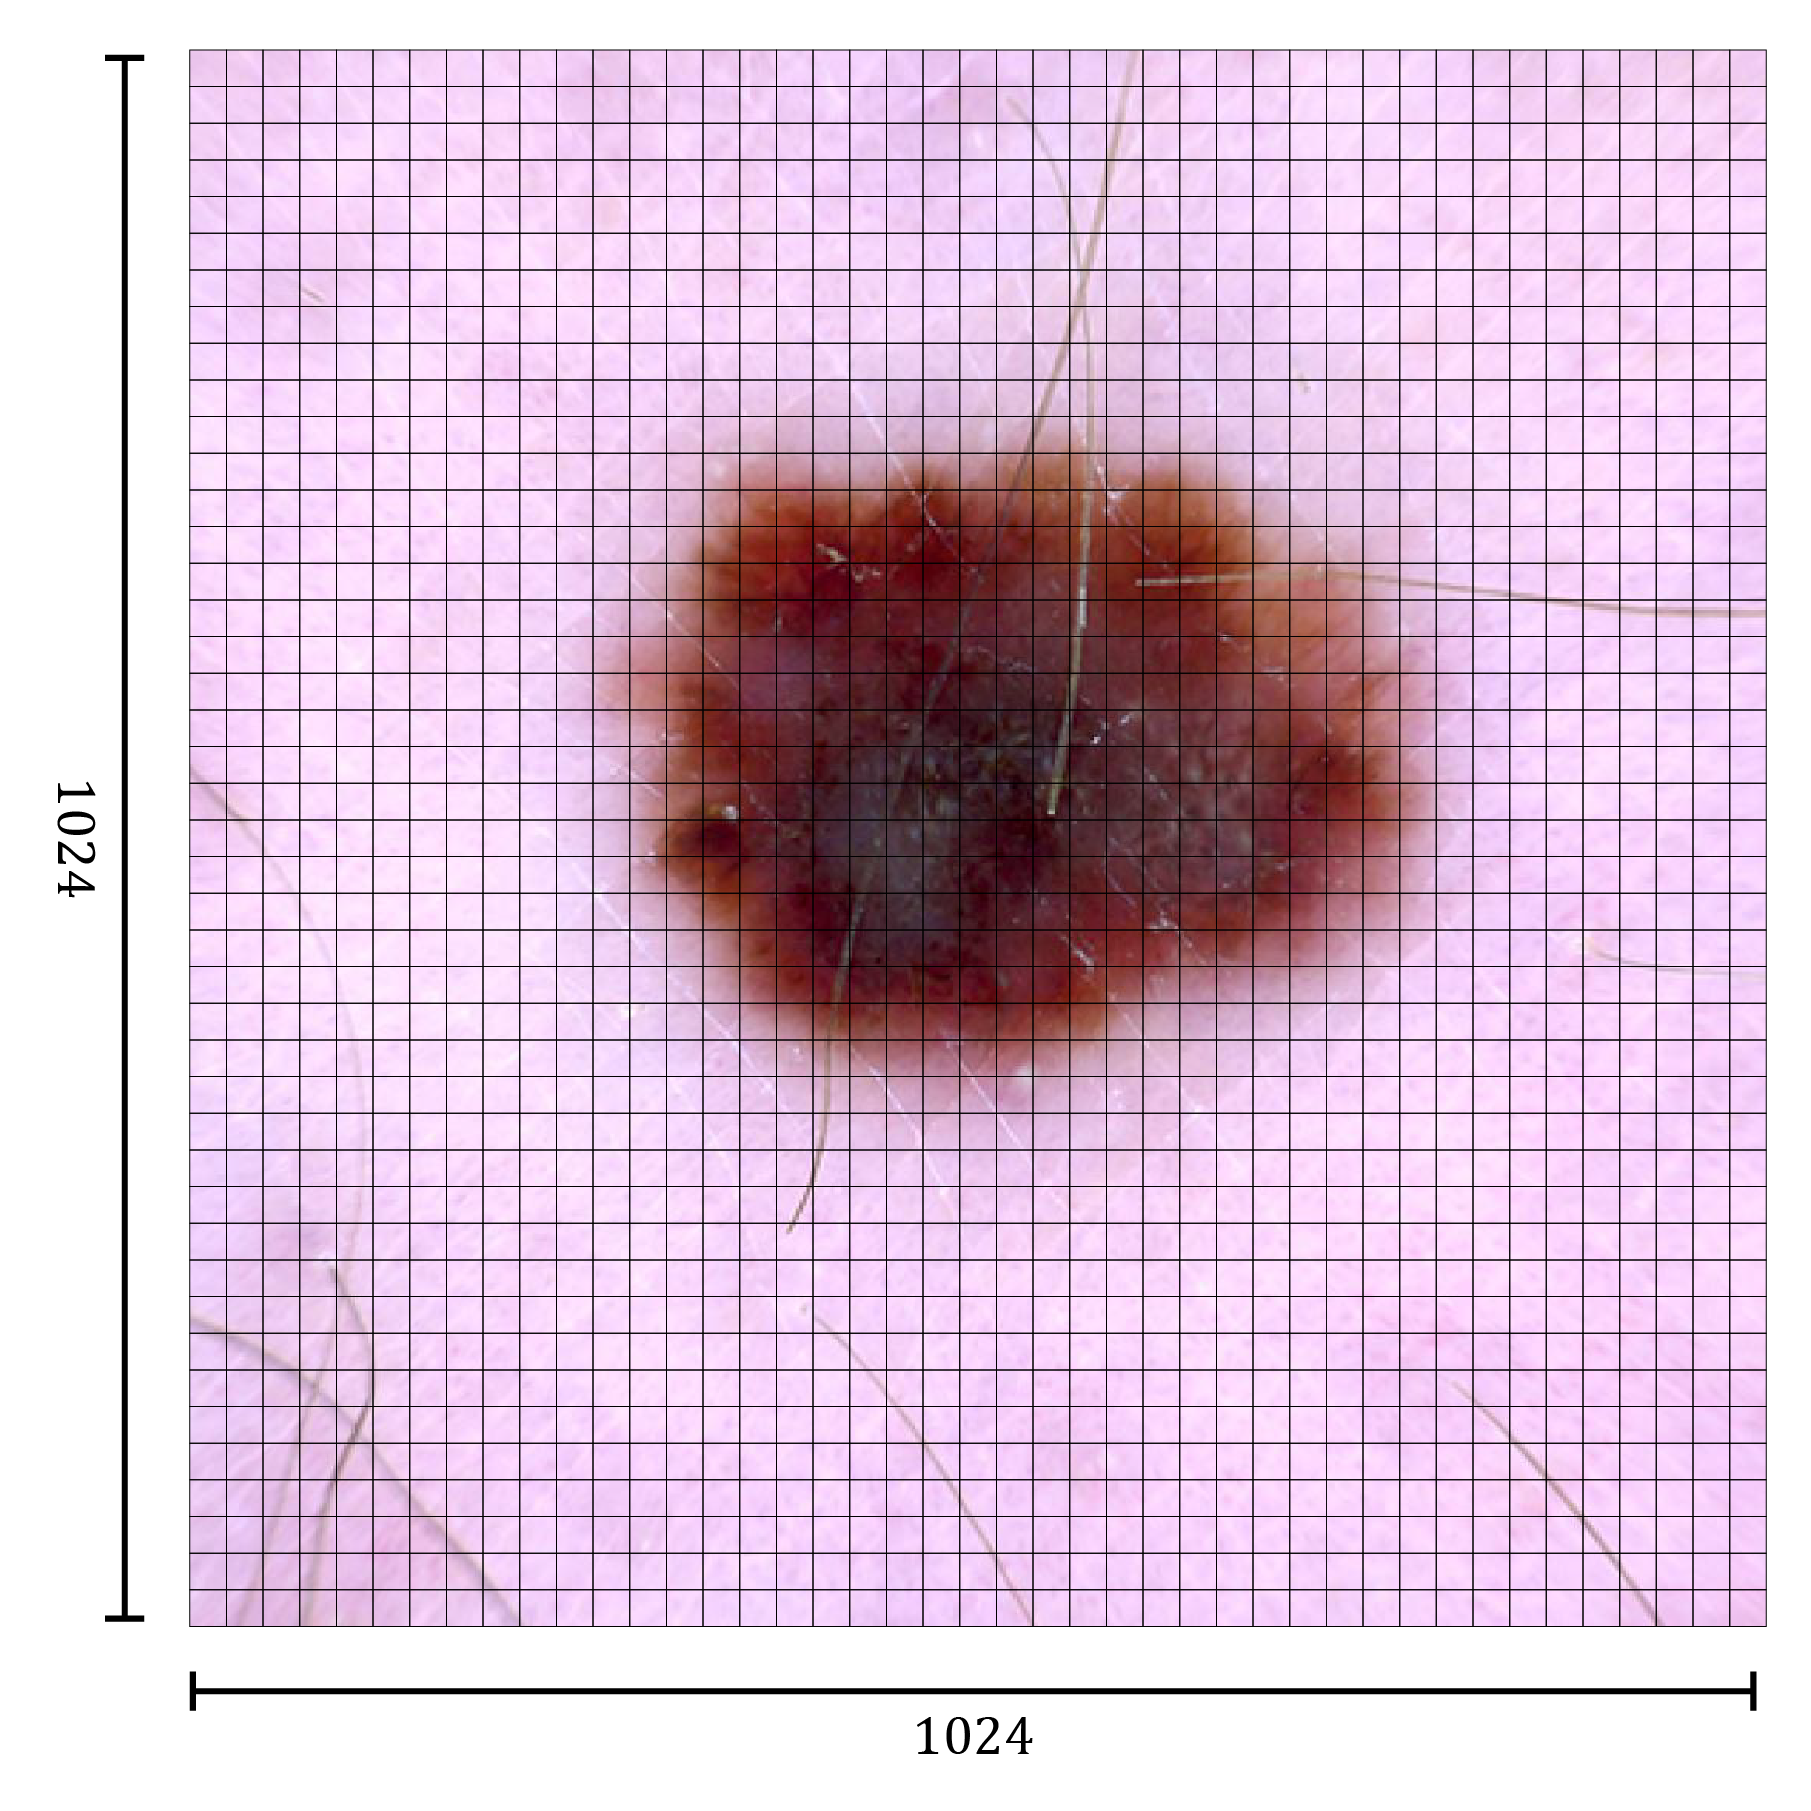
\includegraphics[width=5cm]{img/bab4/resize-1024.png}
            &
            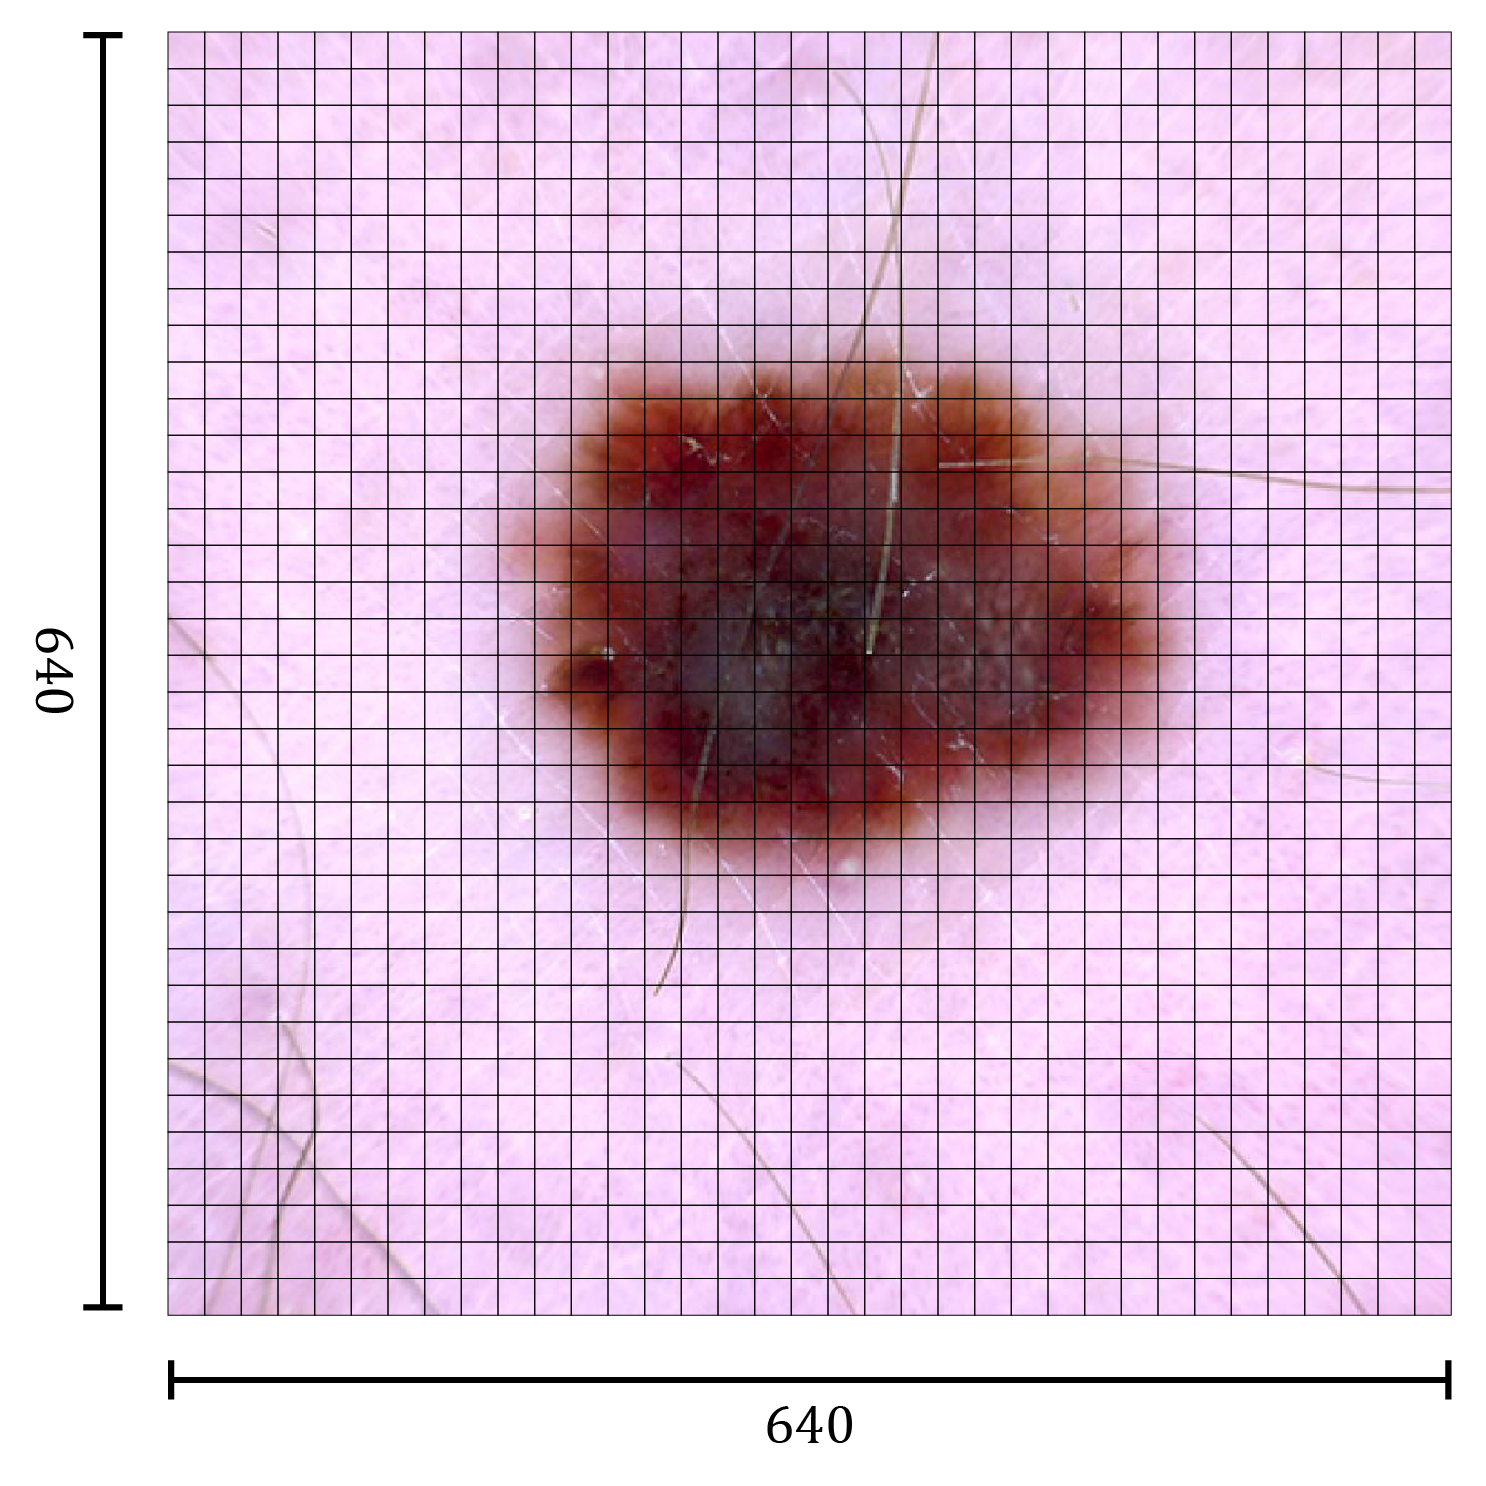
\includegraphics[width=5cm]{img/bab4/resize-640.png} \\
            (a)
            &
            (b) \\
        \end{tabular}
        \caption{\textit{Preprocessing} menggunakan \textit{resize} (a) Citra kanker kulit sebelum dilakukan \textit{resize}; (b) Citra kanker kulit setelah dilakukan \textit{resize}}
        \label{fig:d-resized}
    \end{figure}

    

    \subsection{\textit{Annotation}}
    \textit{Annotation} merupakan proses untuk memberikan label \textit{bounding box} pada citra. Hal ini berguna untuk memberikan informasi spasial mengenai objek yang ada pada citra sehingga YOLO dapat mempelajari dimana letak objek yang terdapat pada suatu citra. \textit{Annotation} dilakukan pada seluruh dataset sehingga dilakukan \textit{annotation} secara manual menggunakan Roboflow sebanyak 1600 citra. Gambar \ref{fig:d-annotation} memperlihatkan nilai yang dibutuhkan untuk melakukan proses \textit{annotation}.

    \begin{figure}[H]
        \centering
            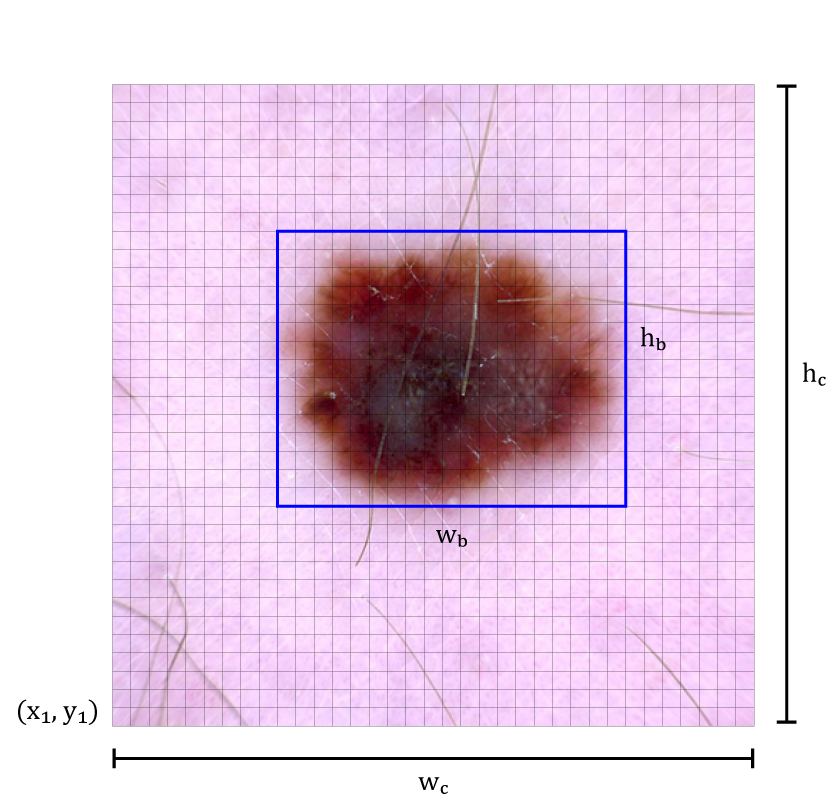
\includegraphics[width=5cm]{img/bab4/annotation.png}
        \caption{Ilustrasi proses \textit{annotation}}
        \label{fig:d-annotation}
    \end{figure}

    Berdasarkan Gambar \ref{fig:d-annotation}, \textit{annotation} dilakukan seperti perhitungan di bawah.

    \begin{alignat*}{5}
        (0) \Rightarrow x       &= \frac{x_1 + \frac{w_b}{2}}{w_c} \qquad\qquad &y  &=\frac{y_1 + \frac{h_b}{2}}{h_c}\\
                                &= \frac{110 + \frac{220}{2}}{640} \qquad\qquad &   &=\frac{80 + \frac{100}{2}}{640}\\
                                &= 0.34 \qquad\qquad                            &   &= 0.20\\
        w                       &= \frac{w_b}{w_c}\qquad\qquad                  &h  &= \frac{h_b}{h_c}\\
                                &= \frac{220}{640}\qquad\qquad                  &   &= \frac{100}{640}\\
                                &= 0.34\qquad\qquad                             &   &= 0.16\\
        (1) \Rightarrow x       &= \frac{x_1 + \frac{w_b}{2}}{w_c}\qquad\qquad  &y  &=\frac{y_1 + \frac{h_b}{2}}{h_c}\\
                                &= \frac{224 + \frac{300}{2}}{640}\qquad\qquad  &   &= \frac{155 + \frac{258}{2}}{640}\\
                                &= 0.58\qquad\qquad                             &   &= 0.44\\
        w                       &= \frac{w_b}{w_c}\qquad\qquad                  &h  &= \frac{h_b}{h_c}\\
                                &= \frac{300}{640}\qquad\qquad                  &   &= \frac{258}{640}\\
                                &= 0.47\qquad\qquad                             &   &= 0.40\\
        \vdots \\
        (1599) \Rightarrow x    &= \frac{x_1 + \frac{w_b}{2}}{w_c}\qquad\qquad  &y  &=\frac{y_1 + \frac{h_b}{2}}{h_c}\\
                                &= \frac{245 + \frac{172}{2}}{640}\qquad\qquad  &   &= \frac{180 + \frac{300}{2}}{640}\\
                                &= 0.58\qquad\qquad                             &   &= 0.50\\
        w                       &= \frac{w_b}{w_c}\qquad\qquad                  &h  &= \frac{h_b}{h_c}\\
                                &= \frac{172}{640}\qquad\qquad                  &   &= \frac{300}{640}\\
                                &= 0.27\qquad\qquad                             &   &= 0.47\\
    \end{alignat*}

    Pada perhitungan di atas, $(x, y)$ merepresentasikan nilai koordinat \textit{bounding box}, $w$ merepresentasikan lebar \textit{bounding box}, dan $h$ merepresentasikan tinggi \textit{bounding box}. Keempat nilai tersebut direpresentasikan dalam bentuk yang sudah dinormalisasi. Hasil dari proses \textit{annotation} seperti terlihat pada Tabel \ref{tab:d-annotation} dimana $c$ merepresentasikan kode kelas yang ada pada dataset.

    \begin{table}[H]
        \caption{\textit{Annotation}}
        \centering
        \begin{tabular}{cccccc}
            \hline
            Index       &$c$        &$x$        &$y$        &$w$        &$h$ \\ \hline
            $0$         &$5$        &$0.34$     &$0.20$     &$0.34$     &$0.16$ \\ \hline
            $1$         &$3$        &$0.58$     &$0.44$     &$0.47$     &$0.40$ \\ \hline
            $2$         &$1$        &$0.12$     &$0.24$     &$0.21$     &$0.21$ \\ \hline
            $3$         &$2$        &$0.63$     &$0.34$     &$0.61$     &$0.34$ \\ \hline
            $4$         &$7$        &$0.28$     &$0.24$     &$0.37$     &$0.30$ \\ \hline
            $\vdots$    &$\vdots$   &$\vdots$   &$\vdots$   &$\vdots$   &$\vdots$ \\ \hline
            $1599$      &$2$        &$0.58$     &$0.50$     &$0.27$     &$0.47$ \\ \hline
        \end{tabular}
        \label{tab:d-annotation}
    \end{table}

\section{Pelatihan Model}
Setelah proses \textit{preprocessing}, citra akan masuk ke tahap \textit{feature learning} dan \textit{object detection} sehingga mendapatkan model terbaik atau bisa disebut proses pelatihan model. Model terbaik didapatkan dari beberapa percobaan yang dilakukan pada proses pelatihan model. Penelitian ini melakukan beberapa percobaan untuk mendapatkan model terbaik. Terdapat tiga jenis percobaan, yaitu uji coba model YOLOv7, uji coba \textit{batch size}, dan uji coba \textit{epochs}. Penelitian ini melakukan uji coba versi YOLOv7, yaitu YOLOv7 dan YOLOv7 Tiny dengan mempertimbangkan waktu komputasi yang dibutuhkan untuk mendapatkan model yang optimal karena YOLOv7 Tiny masih mempertahankan arsitektur YOLOv4 dan memiliki arsitektur yang tidak lebih kompleks daripada YOLOv7. Hal ini akan sangat mempengaruhi waktu komputasi. \textit{Batch size} juga dilakukan uji coba untuk mendapatkan nilai yang optimal dengan akurasi tinggi pada proses pelatihan model. Penelitian ini menggunakan beberapa nilai \textit{batch size}, yaitu 32, 64, dan 128. Uji coba terakhir pada penelitian ini, yaitu \textit{epochs} dengan mempertimbangkan waktu komputasi dan akurasi yang meningkat seiring bertambahnya \textit{epochs}. Penelitian ini menggunakan beberapa nilai \textit{epochs}, yaitu 300, 600, dan 1200.
    \subsection{\textit{Convolutional Layer}}
    Sebagian besar arsitektur YOLOv7 tersusun dari \textit{convolutional layer} seperti terlihat pada Gambar \ref{fig:yolov7-archi}. Setiap operasi konvolusi pada YOLOv7 dilengkapi dengan \textit{Batch Normalization} dan fungsi aktivasi \textit{Sigmoid-weighted Linear Unit}. Pada \textit{convolutiona layer} terjadi proses pembelajaran fitur dari citra masukan dan \textit{feature map} dengan \textit{filter} yang ada pada YOLOv7. YOLOv7 menggunakan 3 operasi konvolusi dengan komposisi yang berbeda pada ukuran \textit{filter} ($f$) dan jumlah \textit{stride} ($s$), yaitu operasi konvolusi dengan $f=1\times 1$ dan $s=1$, $f=3\times 3$ dan $s=1$, $f=3\times 3$ dan $s=2$. Nilai $f$ dan $s$ ditentukan oleh arsitektur YOLOv7. Sedangkan \textit{padding} $(p)$ pada seluruh \textit{convolutional layer} di YOLOv7 bernilai 1 kecuali \textit{maxpool layer} yang tidak menggunakan \textit{padding}. Nilai yang ada pada \textit{filter} ditentukan secara acak oleh arsitektur YOLOv7 yang terdiri dari 3 lapisan sesuai dengan data masukan yang berupa citra RGB dengan 3 kanal. Contoh perhitungan \textit{convolutional layer} menggunakan data masukan citra RGB kanker kulit berukuran $640\times 640$ dengan 32 \textit{filter} berukuran $3\times 3$ pada masing-masing kanal RGB seperti terlihat pada Gambar \ref{fig:d-convol}.

    \begin{figure}[H]
        \centering
            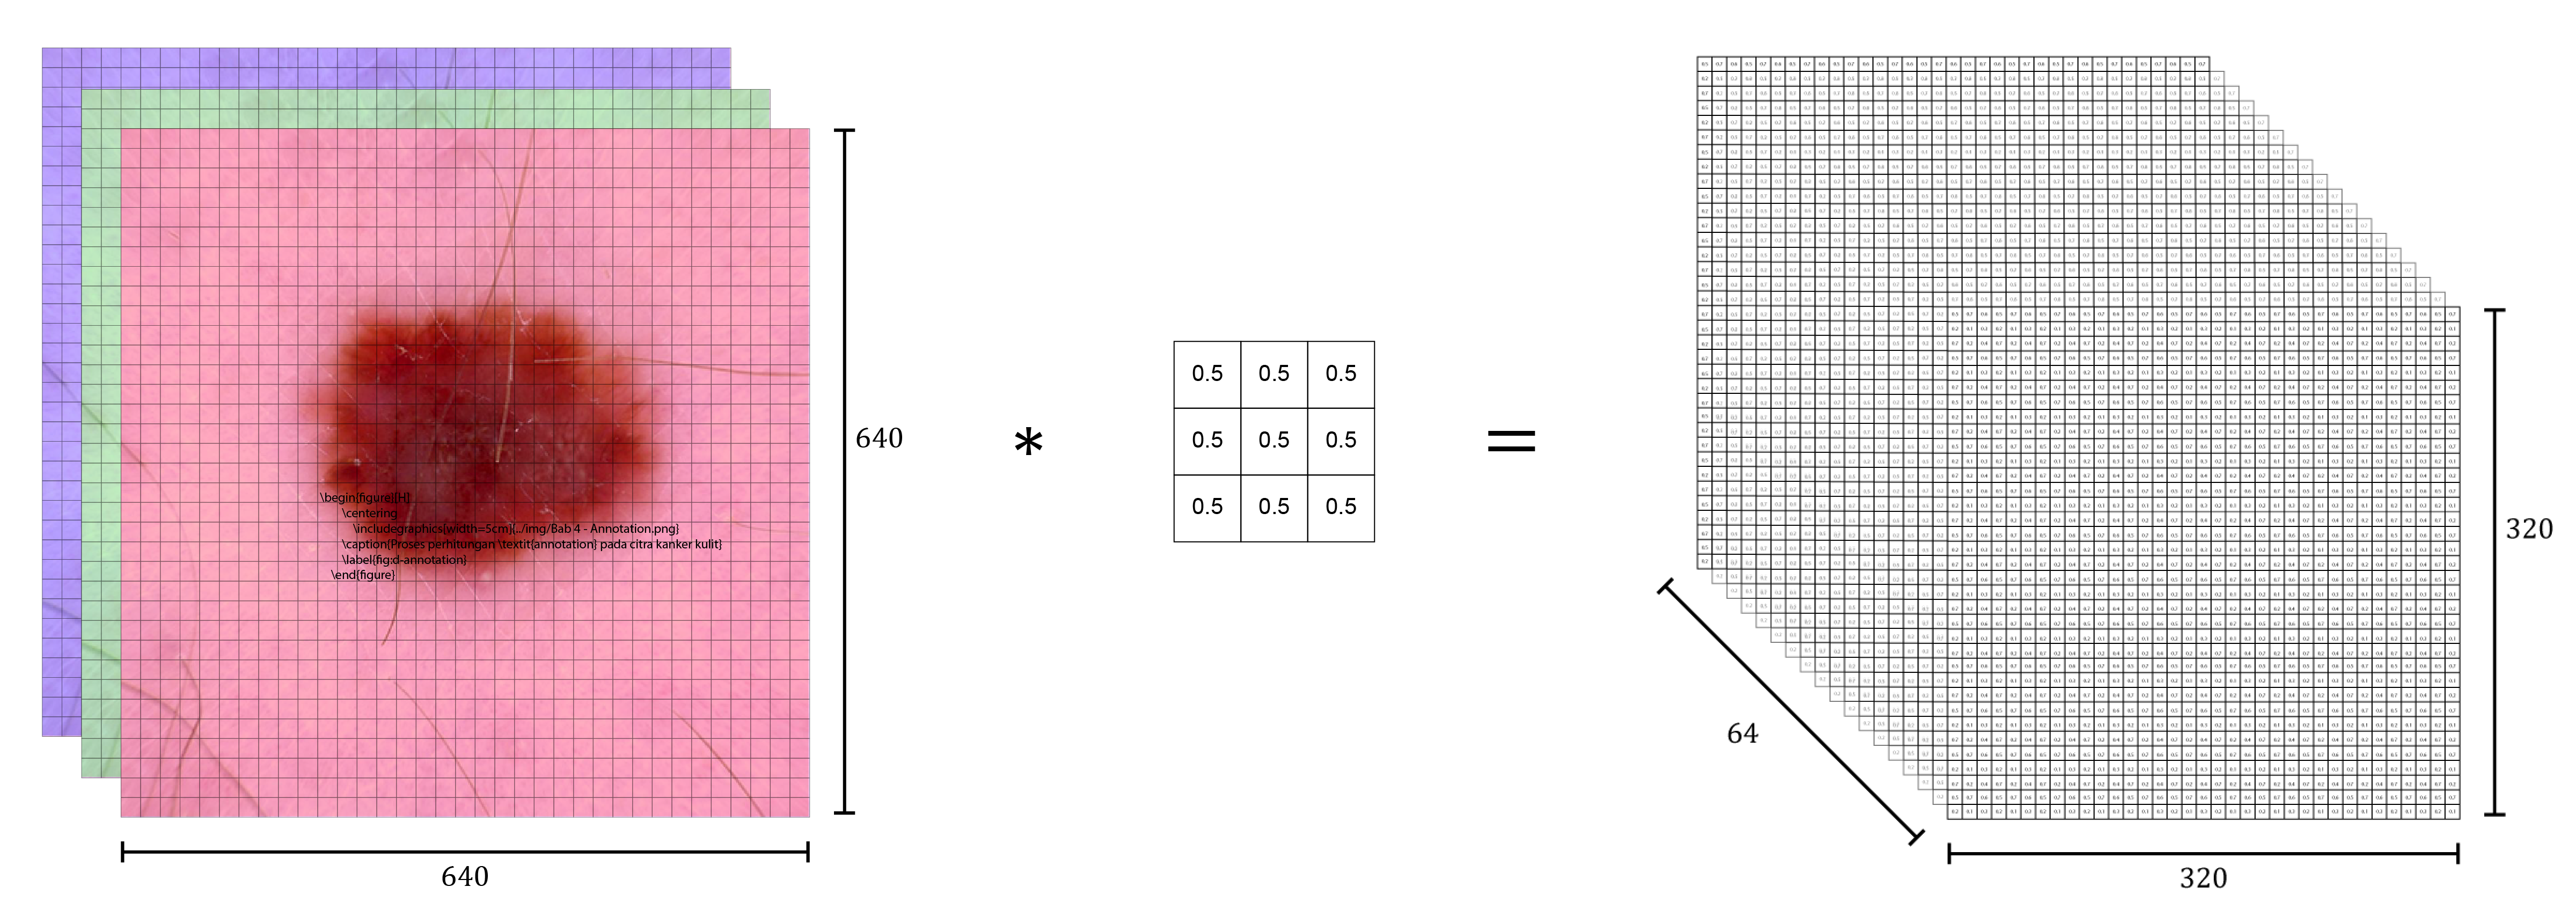
\includegraphics[width=10cm]{img/bab4/convolution.png}
        \caption{Ilustrasi operasi konvolusi data masukan dengan \textit{filter} yang menghasilkan \textit{feature map}}
        \label{fig:d-convol}
    \end{figure}

    Seperti terlihat pada Gambar \ref{fig:d-convol}, operasi konvolusi antara data masukan dengan \textit{filter} yang sudah ditentukan oleh YOLOv7 akan menghasilkan \textit{feature map}. Pada \textit{convolution layer} pertama, YOLOv7 menggunakan ukuran \textit{filter} $3\times 3$ dengan $s=1$. Ukuran dan dimensi dari \textit{feature map} dapat dihitung sesuai dengan perhitungan di bawah ini.

    \begin{align*}
        w &= \frac{w - f + 2p}{s} + 1\\
        &= \frac{640 - 3 + 2(1)}{1} + 1\\
        &= 640
    \end{align*}

    Perhitungan di atas memperlihatkan bahwa ukuran \textit{feature map} dari operasi konvolusi data masukan berukuran $640\times 640$ terhadap \textit{filter} berukuran $3\times 3$ dengan $s=1$ dan $p=1$ menghasilkan \textit{feature map} berukuran $640\times 640$ piksel. Pada arsitektur YOLOv7 seperti terlihat pada Gambar \ref{fig:yolov7-archi}, \textit{layer} pertama pada YOLOv7 menghasilkan 32 \textit{feature map} dengan ukuran $640\times 640$ piksel. Ilustrasi perhitungan operasi konvolusi data masukan dengan \textit{filter} pada \textit{layer} pertama di YOLOv7 dapat dicontohkan seperti di bawah ini.

    \begin{alignat*}{5}
        R_{(0, 0)}          &=  &&\bigl( I_{r}(0, 0)\times F_{r}(0, 0) + I_{r}(0, 1)\times F_{r}(0, 1) + I_{r}(0, 2)\times F_{r}(0, 2) + \cdots + \\
                            &   &&I_{r}(2, 2)\times F_{r}(2, 2) \bigr) + \bigl( I_{g}(0, 0)\times F_{g}(0, 0) + I_{g}(0, 1)\times F_{g}(0, 1) + \\
                            &   &&I_{g}(0, 2)\times F_{g}(0, 2) + \cdots + I_{g}(2, 2)\times F_{g}(2, 2) \bigr) + \bigl( I_{b}(0, 0)\times F_{b}(0, 0) + \\
                            &   &&I_{b}(0, 1)\times F_{b}(0, 1) + I_{b}(0, 2)\times F_{b}(0, 2) + \cdots + I_{b}(2, 2)\times F_{b}(2, 2) \bigr) \\
        % === Batas rumus
                            &=  &&\bigl( (0.925490\times 0.19116) + (0.925490\times 0.17358) + (0.925490\times \\
                            &   &&0.17896) + \cdots + (0.913725\times 0.13184) \bigr) + \bigl( (0.776471\times 0.19116) + \\
                            &   &&(0.776471\times 0.17358) + (0.776471\times 0.17896) + \cdots + (0.764706\times \\
                            &   &&0.13184) \bigr) + \bigl( (0.937255\times 0.19116) + (0.937255\times 0.17358) + \\
                            &   &&(0.937255\times 0.17896) + \cdots + (0.925490\times 0.13184) \bigr) \\
                            &=  &&0.404922 \\
        \vdots \\
        R_{(639, 639)}      &=  &&\bigl( I_{r}(638, 638)\times F_{r}(638, 638) + I_{r}(638, 639)\times F_{r}(638, 639) + \\
                            &   &&I_{r}(638, 640)\times F_{r}(638, 640) + \cdots + I_{r}(640, 640)\times F_{r}(640, 640) \bigr) + \\
                            &   &&\bigl( I_{g}(638, 638)\times F_{g}(638, 638) + I_{g}(638, 639)\times F_{g}(638, 639) + \\
                            &   &&I_{g}(638, 640)\times F_{g}(638, 640) + \cdots + I_{g}(640, 640)\times F_{g}(640, 640) \bigr) + \\
                            &   &&\bigl( I_{b}(638, 638)\times F_{b}(638, 638) + I_{b}(638, 639)\times F_{b}(638, 639) + \\
                            &   &&I_{b}(638, 640)\times F_{b}(638, 640) + \cdots + I_{b}(640, 640)\times F_{b}(640, 640) \bigr) \\
        % === Batas Rumus
                            &=  &&\bigl( (0.941176\times 0.19116) + (0.945098\times 0.17358) + (0.937255\times \\
                            &   &&0.17896) + \cdots + (0.949020\times 0.13184) \bigr) + \bigl( (0.760784\times 0.19116) + \\
                            &   &&(0.764706\times 0.17358) + (0.756863\times 0.17896) + \cdots + (0.768627\times \\
                            &   &&0.13184) \bigr) + \bigl( (0.941176\times 0.19116) + (0.945098\times 0.17358) + \\
                            &   &&(0.937255\times 0.17896) + \cdots + (0.949020\times 0.13184) \bigr) \\
                            &=  &&0.258519 \\
    \end{alignat*}

    Perhitungan di atas akan menghasilkan \textit{feature map} hasil dari operasi data masukan dengan \textit{filter} sebagaimana matriks di bawah ini. Matriks di bawah adalah salah satu dari 32 \textit{feature map} dengan ukuran $640\times 640$ yang dihasilkan dari operasi konvolusi pada perhitungan di atas.

    \begin{align*}
        R_{(:, :, 0)} = 
        \begin{pmatrix}
            0.404922 & 0.445536 & 0.445536 & 0.445536 & \cdots & 0.458136 \\
            0.349199 & 0.309777 & 0.309777 & 0.309777 & \cdots & 0.326002 \\
            0.348241 & 0.309294 & 0.309294 & 0.309294 & \cdots & 0.326987 \\
            0.348800 & 0.310123 & 0.310123 & 0.310123 & \cdots & 0.340638 \\
            0.350666 & 0.311744 & 0.311837 & 0.311837 & \cdots & 0.337295 \\
            \vdots   & \vdots   & \vdots   & \vdots   & \ddots &\vdots \\
            0.265303 & 0.246458 & 0.250151 & 0.255221 & \cdots & 0.258519 \\
        \end{pmatrix}_{640\times 640}
    \end{align*}

    Visualisasi 32 \textit{feature map} hasil dari operasi konvolusi pada perhitungan di atas seperti terlihat pada Gambar \ref{fig:d-feamap}.

    \begin{figure}[H]
        \begin{center}
            \includegraphics[width=12cm]{img/bab4/conv-layer.png}
            \caption{Visualisasi \textit{feature map} pada YOLOv7}
            \label{fig:d-feamap}
        \end{center}
    \end{figure}
    
    \subsection{\textit{Batch Normalization}}

    Setelah mendapatkan hasil \textit{feature map}, YOLOv7 mengubah \textit{feature map} tersebut ke dalam bentuk yang dinormalisasi dengan menggunakan \textit{batch normalization}. Perhitungan \textit{batch normalization} dilakukan menggunakan Persamaan \ref{eq:bn-4} dimana $\mu = -0.002345$, $\sigma^2 = 29.41072$, $\epsilon = 0.001$, $\gamma = 1.0021$, dan $\beta = 1.624$. Perhitungan \textit{batch normalization} seperti terlihat di bawah.

    \begin{align*}
        \breve{Z}_{0, 0}     &= \gamma \left( \frac{Z_{i} - \mu}{\sqrt{\sigma^2 - \epsilon}} \right) + \beta \\
                             &= 1.0021 \left( \frac{0.404922 - (-0.002345)}{\sqrt{29.41072 - 0.001}} \right) + 1.624\\
                             &= -0.589056\\
        \vdots\\
        \breve{Z}_{639, 639} &= \gamma \left( \frac{Z_{i} - \mu}{\sqrt{\sigma^2 - \epsilon}} \right) + \beta \\
                             &= 1.0021 \left( \frac{0.258519 - (-0.002345)}{\sqrt{29.41072 - 0.001}} \right) + 1.624\\
                             &= -5.816965\\
    \end{align*}

    Hasil perhitungan masing-masing nilai untuk \textit{batch normalization} seperti terlihat pada matriks di bawah ini.

    \begin{align*}
        R_{(:, :, 0)} = 
        \begin{pmatrix}
            -0.589056 & 0.861231  & 0.861231  & 0.861231  & \cdots & -0.807409 \\
            -2.578891 & -3.986590 & -3.986590 & -3.986590 & \cdots & -2.776101 \\
            -2.613092 & -4.003831 & -4.003831 & -4.003831 & \cdots & -2.778702 \\
            -2.593120 & -3.974232 & -3.974232 & -3.974232 & \cdots & -2.884571 \\
            -2.526499 & -3.916370 & -3.913023 & -3.913023 & \cdots & -3.003972 \\
            \vdots    & \vdots    & \vdots    & \vdots    & \ddots & \vdots \\
            -5.574710 & -6.247649 & -6.115799 & -5.934733 & \cdots & -5.816965 \\
        \end{pmatrix}_{640\times 640}
    \end{align*}

    Nilai pada \textit{feature map} hasil normalisasi memiliki interval yang tidak terlalu jauh seperti terlihat pada matriks di atas. Visualisasi \textit{feature map} yang telah melewati \textit{batch normalization layer} seperti terlihat pada Gambar \ref{fig:d-banorm}.

    \begin{figure}[H]
        \begin{center}
            \includegraphics[width=12cm]{img/bab4/bn-layer.png}
            \caption{Visualisasi \textit{feature map} setelah melewati \textit{batch normalization layer} pada YOLOv7}
            \label{fig:d-banorm}
        \end{center}
    \end{figure}

    \subsection{\textit{Leaky Rectified Linear Unit} (Leaky ReLU)}

    YOLOv7 Tiny menggunakan Leaky ReLU untuk fungsi aktivasi pada setiap \textit{layer} di arsitekturnya. Hal ini akan mengurangi waktu komputasi jika dibandingkan dengan fungsi aktivasi SiLU. Fungsi aktivasi Leaky ReLU menerima sedikit nilai negatif dengan grafik menaik secara konstan seperti terlihat pada Gambar \ref{fig:l-relu}. Perhitungan fungsi aktivasi Leaky ReLU menggunakan Persamaan \ref{eq:l-relu} seperti terlihat di bawah ini.

    \begin{align*}
        f(x)_{(0, 0)}       &= max(0.1\times x, x) \\
                            &= max(0.1\times (-0.589056), -0.589056) \\
                            &= max(0.1\times (-0.589056), -0.589056) \\
                            &= -0.005891 \\
        \vdots \\
        f(x)_{(639, 639)}   &= max(0.1\times x, x) \\
                            &= max(0.1\times (-5.816965), -5.816965) \\
                            &= max(0.1\times (-5.816965), -5.816965) \\
                            &= -0.058170 \\
    \end{align*}

    Hasil \textit{feature map} yang telah diaktivasi menggunakan Leaky ReLU seperti terlihat di bawah ini.

    \begin{align*}
        R_{(:, :, 0)} = 
        \begin{pmatrix}
            -0.005891 & 0.861231  & 0.861231  & 0.861231  & \cdots & -0.008074 \\
            -0.025789 & -0.039866 & -0.039866 & -0.039866 & \cdots & -0.027761 \\
            -0.026131 & -0.040038 & -0.040038 & -0.040038 & \cdots & -0.027787 \\
            -0.025931 & -0.039742 & -0.039742 & -0.039742 & \cdots & -0.028846 \\
            -0.025265 & -0.039164 & -0.039130 & -0.039130 & \cdots & -0.030040 \\
            \vdots    & \vdots    & \vdots    & \vdots    & \ddots & \vdots \\
            -0.055747 & -0.062476 & -0.061158 & -0.059347 & \cdots & -0.058170 \\
        \end{pmatrix}_{640\times 640}
    \end{align*}

    Perhitungan fungsi aktivasi Leaky ReLU terjadi hingga pada \textit{feature map} terakhir. Visualisasi \textit{feature map} yang telah melewati fungsi aktivasi Leaky ReLU seperti terlihat pada Gambar \ref{fig:d-lrelu}.

    \begin{figure}[H]
        \begin{center}
            \includegraphics[width=12cm]{img/bab4/lrelu-layer.png}
            \caption{Visualisasi \textit{feature map} setelah melewati fungsi aktivasi Leaky ReLU pada YOLOv7}
            \label{fig:d-lrelu}
        \end{center}
    \end{figure}

    \subsection{\textit{Sigmoid-weighted Linear Unit} (SiLU)}
    Peningkatan yang paling utama dari YOLOv7 adalah fungsi aktivasi SiLU. Hal ini juga meningkatkan waktu komputasi karena fungsi aktivasi SiLU memiliki persamaan yang lebih kompleks daripada fungsi aktivasi Leaky ReLU. Dapat dilihat pada Gambar \ref{fig:silu} bahwa grafik terlihat menaik dengan tidak konstan. Meskipun hal ini meningkatkan waktu komputasi, namun SiLU dapat meningkatkan akurasi pada YOLOv7. Perhitungan fungsi aktivasi SiLU menggunakan Persamaan \ref{eq:silu} seperti terlihat di bawah ini.

    \begin{align*}
        a_k(z_k)_{(0, 0)}       &= z_k\frac{1}{1+e^{-(z_k)}} \\
                                &= -0.589056\frac{1}{1+2.718^{0.589056}} \\
                                &= -0.210206 \\
        \vdots \\
        a_k(z_k)_{(319, 319)}   &= z_k\frac{1}{1+e^{-(z_k)}} \\
                                &= -5.816965\frac{1}{1+2.718^{5.816965}} \\
                                &= -0.017264 \\
    \end{align*}

    Hasil \textit{feature map} yang telah melewati fungsi aktivasi SiLU seperti terlihat pada matriks di bawah ini.

    \begin{align*}
        R_{(:, :, 0)} = 
        \begin{pmatrix}
            -0.210206 & 0.605375  & 0.605375  & 0.605375  & \cdots & -0.249040 \\
            -0.181836 & -0.072654 & -0.072654 & -0.072654 & \cdots & -0.162761 \\
            -0.178476 & -0.071743 & -0.071743 & -0.071743 & \cdots & -0.162515 \\
            -0.180436 & -0.073313 & -0.073313 & -0.073313 & \cdots & -0.152656 \\
            -0.187015 & -0.076465 & -0.076651 & -0.076651 & \cdots & -0.141928 \\
            \vdots    & \vdots    & \vdots    & \vdots    & \ddots & \vdots \\
            -0.021063 & -0.012066 & -0.013472 & -0.015661 & \cdots & -0.017264 \\
        \end{pmatrix}_{320\times 320}
    \end{align*}

    Perhitungan fungsi aktivasi SiLU terjadi hingga pada lapisan terakhir. Visualisasi \textit{feature map} yang telah melewati fungsi aktivasi Silu seperti terlihat pada Gambar \ref{fig:d-silu}.

    \begin{figure}[H]
        \begin{center}
            \includegraphics[width=12cm]{img/bab4/silu-layer.png}
            \caption{Visualisasi \textit{feature map} setelah melewati fungsi aktivasi SiLU pada YOLOv7}
            \label{fig:d-silu}
        \end{center}
    \end{figure}

    \subsection{\textit{Pooling Layer}}

    \textit{Pooling layer} berguna untuk mengurangi ukuran \textit{feature map} sehingga dapat mempercepat waktu komputasi pada saat pelatihan model YOLOv7. \textit{Pooling layer} mengurangi ukuran pada masing-masing \textit{feature map} tanpa menghilangkan informasi yang penting dari \textit{feature map}. Arsitektur YOLOv7 menggunakan \textit{max-pooling} dimana \textit{max-pooling} mengambil nilai maksimum pada ukuran \textit{filter} tertentu. Arsitektur YOLOv7 menggunakan ukuran \textit{filter} $2\times 2$ untuk mengimplementasikan \textit{pooling layer}. Berdasarkan hasil \textit{feature map} fungsi aktivasi SiLU, perhitungan \textit{pooling layer} untuk setiap nilainya seperti terlihat di bawah ini.

    \begin{align*}
        P_{(0, 0)}      &= max(-0.210206, 0.605375, -0.181836, -0.072654)\\
                        &= 0.605375 \\
        \vdots \\
        P_{(319, 319)}  &= max(-0.087075, -0.128279, -0.017056, -0.017264)\\
                        &= -0.128279 \\
    \end{align*}

    Hasil \textit{feature map} setelah melewati \textit{pooling layer} seperti terlihat di bawah ini.

    \begin{align*}
        R_{(:, :, 0)} = 
        \begin{pmatrix}
            0.605375  & -0.143407 & -0.139577 & -0.148889 & \cdots & -0.221489 \\
            -0.185320 & -0.084338 & -0.053553 & -0.076679 & \cdots & -0.146808 \\
            -0.206630 & -0.090965 & -0.077647 & -0.070564 & \cdots & -0.187663 \\
            -0.201531 & -0.089601 & -0.077569 & -0.064958 & \cdots & -0.194047 \\
            -0.202485 & -0.085817 & -0.061791 & -0.076593 & \cdots & -0.189475 \\
            \vdots    & \vdots    & \vdots    & \vdots    & \ddots & \vdots \\
            -0.192949 & -0.270050 & -0.256753 & -0.253126 & \cdots & -0.128279 \\
        \end{pmatrix}_{80, 80}
    \end{align*}

    Visualisasi \textit{feature map} yang telah melewati \textit{max-pooling layer} seperti terlihat pada Gambar \ref{fig:d-maxpool}.

    \begin{figure}[H]
        \begin{center}
            \includegraphics[width=12cm]{img/bab4/mp-layer.png}
            \caption{Visualisasi \textit{feature map} setelah melewati \textit{max-pooling layer} pada YOLOv7}
            \label{fig:d-maxpool}
        \end{center}
    \end{figure}

    \subsection{\textit{Upsample Layer}}

    Proses untuk mengembalikan ukuran \textit{feature map} dapat dilakukan menggunakan \textit{upsample layer}. \textit{Upsample layer} mengembalikan ukuran \textit{feature map} seperti pada ukuran sebelumnya. \textit{Unpooling layer} adalah nama lain dari \textit{upsample layer}. Sehingga, \textit{upsample layer} dapat diimplementasikan setelah \textit{feature map} melewati \textit{downsample layer} atau \textit{pooling layer} untuk mengurangi waktu komputasi. Perhitungan \textit{upsample layer} pada YOLOv7 menggunakan metode \textit{nearest} atau mempertimbangkan nilai piksel di sekitarnya untuk melakukan \textit{upsample}. Ilustrasi \textit{upsample layer} seperti terlihat pada Gambar \ref{fig:il-nearest}. \textit{Upsample layer} pada arsitektur YOLOv7 terletak setelah banyak proses konvolusi dan \textit{max-pool} sehingga \textit{feature map} yang telah melewati \textit{upsample layer} memiliki ukuran $40\times 40$ seperti di bawah ini.

    \begin{align*}
        R_{(40, 40, 0)} = 
        \begin{pmatrix}
            -0.240868 & -0.240868 & -0.240287 & -0.240287 & \cdots & -0.238043 \\
            -0.240868 & -0.240868 & -0.240287 & -0.240287 & \cdots & -0.238043 \\
            -0.244172 & -0.244172 & -0.240042 & -0.240042 & \cdots & -0.240131 \\
            -0.244172 & -0.244172 & -0.240042 & -0.240042 & \cdots & -0.240131 \\
            -0.251152 & -0.251152 & -0.236841 & -0.236841 & \cdots & -0.256989 \\
            \vdots    & \vdots    & \vdots    & \vdots    & \ddots & \vdots \\
            -0.262205 & -0.262205 & -0.264320 & -0.264320 & \cdots & -0.242232 \\
        \end{pmatrix}
    \end{align*}

    Visualisasi \textit{feature map} yang telah melewati \textit{upsample layer} seperti terlihat pada Gambar \ref{fig:d-uplayer}.

    \begin{figure}[H]
        \begin{center}
            \includegraphics[width=12cm]{img/bab4/up-layer.png}
            \caption{Visualisasi \textit{feature map} setelah melewati \textit{upsample layer} pada YOLOv7}
            \label{fig:d-uplayer}
        \end{center}
    \end{figure}

    \subsection{\textit{Efficient Layer Aggregation Networks (ELAN)}}

    Pada YOLOv7, terdapat 8 jaringan ELAN dengan struktur masing-masing menggunakan \textit{Convolutional Layer}, \textit{Batch Normalization}, dan \textit{Sigmoid-weighted Linear Unit} (CBS). Jaringan ELAN memiki operasi konvolusi yang bertumpuk hingga pada layer terakhir digabungkan dengan hasil keluaran dari layer awal sehingga meningkatkan pembelajaran fitur pada YOLOv7. ELAN terdiri dari $2\times CBS$ di bagian awal untuk mengurangi dimensi \textit{feature map} karena menggunakan ukuran \textit{filter} $1\times 1$ dengan $s = 1$. Kemudian terdapat 4 \textit{layer} untuk pembelajaran fitur menggunakan filter berukuran \textit{filter} $3\times 1$ dengan $s = 1$. Pada bagian akhir struktur ELAN, terdapat \textit{Concatenation Layer} yang berguna untuk menggabungkan semua hasil pembelajaran fitur pada \textit{layer} sebelumnya sehingga menghasilkan \textit{feature map} baru. Visualisasi \textit{feature map} yang telah melewati jaringan \textit{ELAN} seperti terlihat pada Gambar \ref{fig:d-elan}.

    \begin{figure}[H]
        \begin{center}
            \includegraphics[width=12cm]{img/bab4/elan-layer.png}
            \caption{Visualisasi \textit{feature map} setelah melewati jaringan \textit{ELAN} pada YOLOv7}
            \label{fig:d-elan}
        \end{center}
    \end{figure}

    \subsection{\textit{Intesection over Union} (IoU)}
    YOLOv7 menggunakan IoU untuk mengetahui keakuratan hasil prediksi model yang telah dilakukan pelatihan model. Hasil prediksi model yang berupa tumpukan \textit{feature map} atau tensor dilakukan pengukuran keakuratan \textit{bounding box} yang telah diprediksi menggunakan IoU terhadap \textit{ground truth}. \textit{Ground truth} merupakah data aktual yang telah diberikan label berupa jenis kanker dan \textit{bounding box}. Perhitungan IoU memerlukan informasi terkait \textit{overlap area} dan \textit{union area} yang dihitung menggunakan Persamaan \ref{eq:oa} dan \ref{eq:ua}. Contoh perhitungan IoU menggunakan Persamaan \ref{eq:iou} seperti terlihat di bawah ini.

    \begin{align*}
        x_{a1} &= max(3, 5)\\
               &= 5\\
        y_{a1} &= max(4, 10)\\
               &= 10\\
        x_{a2} &= min(13, 17)\\
               &= 13\\
        y_{a2} &= min(15, 19)\\
               &= 15\\
        OA     &= (13-5)\times (15-10)\\
               &= 40\\
        UA     &= (13-3)\times (15-4) + (17-5)\times (19-10) - 40\\
               &= 178\\
        IoU    &= \frac{40}{178}\\
               &= 0.224
    \end{align*}

    Seperti terlihat pada perhitungan di atas, nilai IoU 0.224 merupakan nilai yang kecil karena mendekati 0. Jika nilai ambang batas yang diberikan adalah 0.5 maka hasil prediksi termasuk ke dalam FP.

\section{Pengujian dan Evaluasi Sistem}
Tingkat keberhasilan model klasifikasi jenis kanker kulit menggunakan YOLOv7 dipengaruhi oleh beberapa faktor terkait metode yang diimplementasikan, antara lain varian metode, ukuran \textit{batch size}, dan \textit{epochs}. Sehingga, penelitian ini melakukan beberapa uji coba untuk mendapatkan model terbaik dengan mempertimbangkan perangkat yang dipakai, yaitu $2\times GPU T100$ dengan total GPU \textit{memory} 30gb. Mempertimbangkan hal tersebut, penelitian ini melakukan uji coba varian YOLOv7, yaitu YOLOv7 dan YOLOv7 Tiny. Pada uji coba \textit{batch size}, penelitian ini menggunakan nilai 32, 64, dan 128. Kemudian uji coba \textit{epochs} dilakukan menggunakan nilai 300, 600, dan 1200. Model terbaik dipilih dengan mempertimbangkan nilai mAP pada semua kelas.

Penelitian ini menggunakan \textit{kaggle notebook} untuk melakukan pelatihan model YOLOv7 sehingga penelitian ini memiliki batas sumber daya dan waktu komputasi sehingga terdapat beberapa uji coba yang tidak bisa diselesaikan. Hal ini memengaruhi uji coba \textit{batch size} pada YOLOv7 sehingga uji coba yang awalnya menggunakan nilai \textit{batch size} 32, 64, dan 128 diubah menjadi 16, 32, dan 40. Meskipun penelitian ini mengurangi nilai \textit{batch size} pada YOLOv7, terdapat uji coba yang tidak dapat terselesaikan, yaitu uji coba YOLOv7 dengan 16 \textit{batch size} dan 1200 \textit{epochs}. Hal ini terjadi karena \textit{runtime} GPU pada \textit{kaggle notebook} maksimal hingga 12 jam. Sedangkan waktu pelatihan model YOLOv7 dengan 16 \textit{batch size} dan 1200 \textit{epochs} melebihi batas waktu 12 jam. Hasil uji coba klasifikasi kanker kulit menggunakan YOLOv7 seperti terlihat pada Tabel \ref{tab:d-testing}.

\begin{table}[H]
    \caption{Hasil uji coba varian YOLOv7, \textit{batch size} dan \textit{epochs} pada penelitian ini}
    \centering
    \begin{tabular}{|c|c|c|c|c|c|c|}
        \hline
        Varian YOLO                  & \textit{Batch Size}  & \textit{Epochs} & \textit{Time (h)}  & P     & R     & mAP\\
        \hline
        \multirow{8}{*}{YOLOv7}      & \multirow{2}{*}{16}  & 300             & 5.847              & 0.632 & 0.656 & 0.661\\ \cline{3-7}
                                     &                      & 600             & 11.755             & 0.752 & 0.769 & 0.778\\ \cline{2-7}
                                     & \multirow{3}{*}{32}  & 300             & 3.439              & 0.699 & 0.693 & 0.715\\ \cline{3-7}
                                     &                      & 600             & 6.806              & 0.776 & 0.606 & 0.695\\ \cline{3-7}
                                     &                      & 1200            & 11.423             & 0.773 & 0.720 & 0.749\\ \cline{2-7}
                                     & \multirow{3}{*}{40}  & 300             & 3.225              & 0.725 & 0.678 & 0.696\\ \cline{3-7}
                                     &                      & 600             & 6.692              & 0.775 & 0.626 & 0.694\\ \cline{3-7}
                                     &                      & 1200            & 11.308             & 0.784 & 0.727 & 0.773\\ \cline{2-7}
        \hline
        \multirow{9}{*}{YOLOv7 Tiny} & \multirow{3}{*}{32}  & 300             & 1.683              & 0.851 & 0.662 & 0.782\\ \cline{3-7}
                                     &                      & 600             & 3.521              & 0.709 & 0.644 & 0.689\\ \cline{3-7}
                                     &                      & 1200            & 7.084              & 0.785 & 0.804 & 0.827\\ \cline{2-7}
                                     & \multirow{3}{*}{64}  & 300             & 1.731              & 0.752 & 0.757 & 0.789\\ \cline{3-7}
                                     &                      & 600             & 3.409              & 0.640 & 0.600 & 0.635\\ \cline{3-7}
                                     &                      & 1200            & 6.763              & 0.698 & 0.606 & 0.669\\ \cline{2-7}
                                     & \multirow{3}{*}{128} & 300             & 1.662              & 0.823 & 0.720 & 0.805\\ \cline{3-7}
                                     &                      & 600             & 3.235              & 0.823 & 0.782 & \textbf{0.832}\\ \cline{3-7}
                                     &                      & 1200            & 6.713              & 0.872 & 0.728 & 0.818\\ \cline{2-7}
        \hline
    \end{tabular}
    \label{tab:d-testing}
\end{table}

Pada Tabel \ref{tab:d-testing}, terlihat bahwa nilai terbaik yang diperoleh model YOLOv7 adalah model YOLOv7 dengan 16 \textit{batch size}, 600 \textit{epochs}, 11.755 jam waktu komputasi, 0.752 nilai \textit{precision}, 0.769 nilai \textit{recall}, dan 0.778 nilai mAP. Hal ini disebabkan oleh komposisi \textit{batch size} dan \textit{epochs} yang baik. Dapat dilihat pada Tabel \ref{tab:d-testing} bahwa nilai \textit{batch size} yang besar harus didukung dengan nilai \textit{epochs} yang besar karena di antara \textit{epochs} 600 dan 1200 terdapat peningkatan mAP yang signifikan. Jika nilai \textit{epochs} ditingkatkan maka tidak menutup kemungkinan untuk meningkatkan akurasi yang lebih signifikan. YOLOv7 memerlukan waktu untuk mempelajari data dengan varian data yang lebih banyak sehingga \textit{batch size} yang besar tidak memberikan kepastian bahwa akurasi akan meningkat. Melainkan harus diiringi oleh kenaikan \textit{epochs}.

Nilai mAP yang tinggi pada YOLOv7 dengan 32 \textit{batch size} dan 300 \textit{epochs} dapat terjadi karena inisialisasi yang lebih stabil dibandingkan dengan model lainnya. Sehingga tidak menutup kemungkinan dengan nilai \textit{epochs} yang sedikit akan menghasilkan akurasi yang baik. Akan tetapi, bisa dikatakan bahwa model tersebut tidak stabil karena akurasi meningkat secara instan. Nilai akurasi yang baik adalah nilai yang meningkat secara bertahap sehingga model mempelajari data dengan baik.

YOLOv7 Tiny memiliki nilai terbaik dengan waktu komputasi yang tidak lama jika dibandingkan dengan waktu komputasi YOLOv7. Seperti terlihat pada Tabel \ref{tab:d-testing}, model terbaik YOLOv7 Tiny didapatkan dengan 128 \textit{batch size}, 600 \textit{epochs}, 3.235 jam waktu komputasi, 0.823 \textit{precision}, 0.782 \textit{recall}, dan 0.832 mAP. Model terbaik ini didapatkan dengan waktu komputasi 8 jam lebih cepat daripada model terbaik yang dihasilkan oleh YOLOv7. Hal ini terjadi karena dua kondisi, yaitu perbedaan jumlah \textit{convolution layer} dan fungsi aktivasi. Fungsi aktivasi Leaky ReLU terbukti memberikan waktu komputasi yang lebih cepat dan tidak menurunkan akurasi yang memberikan dampak signifikan pada model. ELAN juga dapat memberikan pengaruh yang signifikan pada YOLOv7 karena ELAN tersusun atas banyak \textit{convolutional layer} yang menghabiskan banyak waktu komputasi. Meskipun ELAN dapat meningkatkan akurasi akan tetapi ELAN membutuhkan waktu komputasi yang lebih. Sedangkan dataset pada penelitian ini sudah dapat dipelajari dengan baik oleh YOLOv7 Tiny dengan waktu komputasi yang tidak terlalu lama.

\begin{figure}[H]
    \begin{center}
        \includegraphics[width=12cm]{img/bab4/confmat-yolov7.png}
        \caption{Hasil \textit{confusion matrix} model terbaik YOLOv7}
        \label{fig:d-confmat-yolov7}
    \end{center}
\end{figure}

Model terbaik YOLOv7 didapatkan dengan 16 nilai \textit{batch size} dan 600 nilai \textit{epochs}. Hasil \textit{confusion matrix} model tersebut seperti terlihat pada Gambar \ref{fig:d-confmat-yolov7}. Seperti terlihat pada Gambar \ref{fig:d-confmat-yolov7}, nilai tertinggi didapatkan oleh kelas VASC. Kanker kulit VASC memiliki ciri khas warna dan bentuk yang signifikan sehingga menjadi kelas yang paling mudah dikenali oleh model YOLOv7. Nilai TP yang rendah didapatkan oleh kelas AK dan SCC. Hal ini juga dapat dipertimbahkan bahwa kanker kulit jenis AK dan SCC memiliki kesamaan dengan area sekitar kulit dan memiliki tepi yang kurang jelas seperti terlihat pada Gambar \ref{fig:ak} dan Gambar \ref{fig:scc}. Hal ini juga dapat dipengaruhi oleh tingkat keparahan jenis kanker yang berbeda-beda. Sedangkan kanker kulit yang berbahaya, yaitu MEL mendapatkan nilai TP sebesar 0.84 yang dapat dikatakan baik untuk klasifikasi. 

\textit{Precision} dan \textit{recall} pada setiap jenis kanker kulit dapat dihitung menggunakan Persamaan \ref{eq:precision} dan \ref{eq:recall}. Perhitungan \textit{precision} dan \textit{recall} seperti terlihat di bawah ini.

\begin{alignat*}{5}
    P_{ak}   &= \frac{TP}{TP+FP}         & R_{ak}   &= \frac{TP}{TP+FP} \\
             &= \frac{0.52}{0.52 + 0.28} &          &= \frac{0.52}{0.52 + 0.4} \\
             &= 0.74                     &          &= 0.75 \\
             &\vdots                     &          &\vdots \\
    P_{vasc} &= \frac{TP}{TP+FP}         & R_{vasc} &= \frac{TP}{TP+FP} \\
             &= \frac{0.95}{0.95 + 0.12} &          &= \frac{0.95}{0.95 + 0.05} \\
             &= 0.97                     &          &= 0.92 \\
\end{alignat*}

Hasil visualisasi \textit{precision} dan \textit{recall} pada model terbaik YOLOv7 seperti terlihat pada Gambar \ref{fig:d-pr-yolov7}.

\begin{figure}[H]
    \begin{center}
        \includegraphics[width=12cm]{img/bab4/pr-yolov7.png}
        \caption{Hasil \textit{precision} dan \textit{recall} model terbaik YOLOv7}
        \label{fig:d-pr-yolov7}
    \end{center}
\end{figure}

Nilai \textit{precision} merepresentasikan tingkat prediksi data negatif sebagai data positif sedangkan nilai \textit{recall} merepresentasikan tingkat prediksi data positif sebagai data negatif. Pada studi kasus diagnosis penyakit, nilai \textit{recall} lebih diutamakan. Hal ini karena \textit{recall} merupakan tingkat sensitifitas model terhadap penyakit tertentu. Pada Gambar \ref{fig:d-pr-yolov7}, terlihat bahwa dari 8 jenis kanker kulit yang diklasifikasikan, nilai \textit{precision} pada semua jenis kanker kulit masih berada di bawah $80\%$ kecuali VASC.  Namun, pada Gambar \ref{fig:d-pr-yolov7} terdapat 3 jenis kanker kulit yang mendekati $80\%$, yaitu DF, MEL, dan NV. Sedangkan nilai \textit{recall} MEL berada di atas $80\%$ beserta jenis kanker NV dan VASC. Nilai \textit{recall} jenis kanker kulit MEL perlu dipertimbangkan karena MEL merupakan jenis kanker kulit paling berbahaya. Nilai \textit{precision} dan \textit{recall} jenis kanker kulit AK dan SCC perlu ditingkatkan lagi dengan menambah \textit{epochs}, data, atau \textit{preprocessing}.

Rendahnya nilai \textit{precision} dan \textit{recall} pada model YOLOv7 dapat dipengaruhi oleh metode YOLOv7 yang tidak dapat melakukan \textit{feature learning} dengan maksimal. Jika YOLOv7 dapat meningkatkan sumber daya pelatihan dengan meningkatkan nilai \textit{epochs} maka tidak menutup kemungkinan bahwa nilai \textit{precision} dan \textit{recall} dapat meningkat. Hal tersebut juga dapat dipengaruhi oleh kurangnya jumlah data pada dataset karena pengembang YOLO mengatakan bahwa jumlah minimal data citra untuk satu kelas adalah 1500 data \citep{Jocher2020}. Sedangkan, penelitian ini hanya menggunakan 200 data pada tiap kelas di dataset. 

\begin{figure}[H]
    \begin{center}
        \includegraphics[width=12cm]{img/bab4/confmat-yolov7tiny.png}
        \caption{Hasil \textit{confusion matrix} model terbaik YOLOv7 Tiny}
        \label{fig:d-confmat-yolov7tiny}
    \end{center}
\end{figure}

Hasi visualisasi \textit{confusion matrix} model YOLOv7 Tiny terbaik seperti terlihat pada Gambar \ref{fig:d-confmat-yolov7tiny}. Nilai TP tertinggi yang dihasilkan dari model YOLOv7 Tiny sebesar $95\%$ oleh jenis kanker kulit NV. Pada model YOLOv7 Tiny, kanker kulit jenis AK dan SCC lebih mudah dikenali daripada kanker kulit DF. Bahkan, kanker kulit jenis AK memiliki nilai TP sebesar $73\%$ pada YOLOv7 Tiny sedangkan kanker kulit jenis DF memiliki nilai TP sebesar $61\%$. Ketiga jenis kanker kulit yang memiliki nilai TP tertinggi adalah MEL, NV, dan VASC. Keberhasilan model dalam mendeteksi jenis kanker kulit dapat dilihat dari nilai \textit{precision} dan \textit{recall} seperti perhitungan di bawah ini.

\begin{alignat*}{5}
    P_{ak}   &= \frac{TP}{TP+FP}         & R_{ak}   &= \frac{TP}{TP+FP} \\
             &= \frac{0.73}{0.73 + 0.26} &          &= \frac{0.73}{0.73 + 0.24} \\
             &= 0.74                     &          &= 0.75 \\
             &\vdots                     &          &\vdots \\
    P_{vasc} &= \frac{TP}{TP+FP}         & R_{vasc} &= \frac{TP}{TP+FP} \\
             &= \frac{0.90}{0.90 + 0.02} &          &= \frac{0.90}{0.90 + 0.08} \\
             &= 0.97                     &          &= 0.92 \\
\end{alignat*}

Hasil visualisasi perhitungan \textit{precision} dan \textit{recall} pada perhitungan di atas dapat dilihat pada Gambar \ref{fig:d-pr-yolov7tiny}.

\begin{figure}[H]
    \begin{center}
        \includegraphics[width=12cm]{img/bab4/pr-yolov7tiny.png}
        \caption{Hasil \textit{precision} dan \textit{recall} model terbaik YOLOv7 Tiny}
        \label{fig:d-pr-yolov7tiny}
    \end{center}
\end{figure}

Gambar \ref{fig:d-pr-yolov7tiny} menunjukkan bahwa model dapat mengenali jenis kanker kulit jenis MEL, NV, dan VASC dengan baik. Pada studi kasus klasifikasi penyakit, nilai \textit{recall} sangat diperhitungkan untuk mengetahui tingkat sensitifitas model terhadap penyakit dengan tidak melupakan nilai \textit{precision}. Pada Gambar \ref{fig:d-pr-yolov7tiny}, nilai \textit{recall} yang tinggi didapatkan oleh kanker kulit jenis NV dan VASC.

Berdasarkan nilai \textit{precision} dan \textit{recall} dapat dihitung nilai mAP menggunakan Persamaan \ref{eq:map}. Contoh perhitungan mAP seperti perhitungan di bawah ini.

\begin{alignat*}{5}
    AP_{ak}     &= &&\sum_{i=0}^{n-1} \left( (R_i - R_{i+1})\times P_i \right) \\
                &= &&\left( (0.97-0.95)\times 0.21 \right) + \left( (0.95-0.91)\times 0.32 \right) + \\
                &  &&\left( (0.91-0.87)\times 0.32 \right) + \cdots + \left( (0.12 - 0.02)\times 0.98 \right) \\
                &= &&0.527 \\
                &  &&\vdots \\
    AP_{vasc}   &= &&\sum_{i=0}^{n-1} \left( (R_i - R_{i+1})\times P_i \right) \\
                &= &&\left( (0.99-0.98)\times 0.25 \right) + \left( (0.98-0.95)\times 0.27 \right) + \\
                &  &&\left( (0.95-0.92)\times 0.41 \right) + \cdots + \left( (0.21 - 0.19)\times 0.96 \right) \\
                &= &&0.93
\end{alignat*}

Hasil visualisasi perhitungan di atas seperti terlihat pada Gambar \ref{fig:d-map}.

\begin{figure}[H]
    \begin{center}
        \includegraphics[width=12cm]{img/bab4/map.png}
        \caption{Hasil mAP model terbaik YOLOv7 dan YOLOv7 Tiny}
        \label{fig:d-map}
    \end{center}
\end{figure}

Pada Gambar \ref{fig:d-map}, nilai mAP yang tinggi didapatkan oleh jenis kanker kulit NV dan VASC pada YOLOv7 maupun YOLOv7 Tiny. Nilai mAP pada jenis kanker paling berbahaya, yaitu MEL juga cukup signifikan. Pada YOLOv7, nilai mAP yang perlu ditingkatkan adalah jenis kanker kulit AK. Akan tetapi, jenis kanker kulit AK memiliki nilai yang tidak terlalu buruk pada model YOLOv7 Tiny. Hal ini dapat dipengaruhi oleh arsitektur model. Pada YOLOv7 Tiny tidak menggunakan ELAN dan fungsi aktivasi SiLU, akan tetapi komposisi \textit{convolutional layer} dengan beberapa \textit{skip connections} dan \textit{concatenation}. Hal ini justru membuat YOLOv7 Tiny dapat mempelajari pola data dari jenis kanker kulit AK. Fungsi aktivasi Leaky ReLU pada YOLOv7 Tiny juga dapat berpengaruh karena fungsi aktivasi SiLU hanya meneruskan nilai yang lebih dari 0. Berbeda dengan fungsi aktivasi SiLU pada YOLOv7 dengan perhitungan yang lebih kompleks seperti terlihat pada Persamaan \ref{eq:silu}. 

Pada model YOLOv7 Tiny, jenis kanker kulit dengan nilai mAP terendah didapatkan oleh jenis kanker kulit DF. Sebaliknya, jenis kanker kulit DF memiliki nilai mAP yang tidak terlalu buruk pada model YOLOv7. Dapat dilihat pada Gambar \ref{fig:d-map} bahwa rata-rata jenis kanker kulit memiliki nilai mAP lebih tinggi pada model YOLOv7 Tiny daripada model YOLOv7. Keunggulan YOLOv7 Tiny juga memiliki waktu komputasi yang lebih cepat. Hal ini disebabkan oleh kompleksitas arsitektur yang ada pada YOLOv7 Tiny lebih rendah daripada kompleksitas arsitektur yang ada pada YOLOv7 dengan mempertimbangkan ELAN dan fungsi aktivasi SiLU. Fungsi aktivas Leaky ReLU cukup baik meningkatkan kinerja model YOLOv7 Tiny. Pada penelitian ini dengan dataset kanker kulit yang terdiri dari 8 kelas, model YOLOv7 Tiny cukup memberikan nilai mAP yang tinggi dengan waktu komputasi yang lebih cepat. Pembaruan yang dibawa oleh Wang, dkk. terkait ELAN dan fungsi aktivasi SiLU belum dapat dirasakan pada penelitian ini.

\section{Integrasi Keilmuan}

Hasil penelitian ini memberikan pengingat yang luar biasa terkait perkembangan zaman. Semakin jauh perkembangan zaman, semakin kompleks permasalahan yang dihadapi. Hal ini linier dengan perkembangan solusi untuk menyelesaikan masalah yang terjadi. Salah satunya adalah perkembangan metode untuk melakukan diagnosis kanker kulit. Selain dari rahmat Allah \textit{subhanallahu wa ta'ala}, hal ini tercapai atas kemauan manusia berusaha dalam menghadapi permasalahan yang ada sebagaimana firman-Nya dalam surat Ar-Ra'd ayat 11:

\begin{flushright}
    \begin{RLtext}
        لَهُۥ مُعَقِّبَٰتٌ مِّنۢ بَيْنِ يَدَيْهِ وَمِنْ خَلْفِهِۦ يَحْفَظُونَهُۥ مِنْ أَمْرِ ٱللَّهِ ۗ إِنَّ ٱللَّهَ لَا يُغَيِّرُ مَا بِقَوْمٍ حَتَّىٰ يُغَيِّرُوا۟ مَا بِأَنفُسِهِمْ ۗ وَإِذَآ أَرَادَ ٱللَّهُ بِقَوْمٍ سُوٓءًا فَلَا مَرَدَّ لَهُۥ ۚ وَمَا لَهُم مِّن دُونِهِۦ مِن وَالٍ
    \end{RLtext}
\end{flushright}

Artinya: "Bagi manusia ada malaikat-malaikat yang selalu mengikutinya bergiliran, di muka dan di belakangnya, mereka menjaganya atas perintah Allah. Sesungguhnya Allah tidak merubah keadaan sesuatu kaum sehingga mereka merubah keadaan yang ada pada diri mereka sendiri. Dan apabila Allah menghendaki keburukan terhadap sesuatu kaum, maka tak ada yang dapat menolaknya; dan sekali-kali tak ada pelindung bagi mereka selain Dia." (Ar-Ra'd: 11).

Ayat tersebut menjelaskan bahwa kesungguhan manusia akan membuahkan hasil. Semua usaha manusia tidak akan ada yang sia-sia sehingga Allah \textit{subhanallahu wa ta'ala} tidak memberikan balasan yang sesuai. Bahkan, Allah \textit{subhanallahu wa ta'ala} tidak akan mengubah keadaan suatu kaum hingga mereka mengubah keadaan yang ada pada diri mereka sendiri. Jika saja manusia tidak berusaha untuk menemukan solusi terkait permasalahan, seperti contoh pada penelitian ini adalah penyakit kanker kulit pasti Allah \textit{subhanallahu wa ta'ala} tidak akan memberikan jalan untuk menemukan metode-metode yang dapat menyelesaikan proses klasifikasi kanker kulit dengan hasil yang cukup baik.

Hasil pada penelitian ini menggambarkan kerja keras umat manusia dalam berlomba-lomba dalam bidang keilmuan. Namun, hal itu tidak akan tercapai jika tidak dengan rahmat Allah \textit{subhanallahu wa ta'ala}. Hal tersebut juga salah satu dari bentuk ikhtiar seorang hamba kepada Allah \textit{subhanallahu wa ta'ala}. Allah \textit{subhanallahu wa ta'ala} yang memilki kuasa atas kesembuhan terkait penyakit yang menimpa sebagaimana firman-Nya dalam surat Asy-Syu'ara ayat 80:

\begin{flushright}
    \<وَإِذَا مَرِضْتُ فَهُوَ يَشْفِينِ>
\end{flushright}

Artinya: "Dan apabila aku sakit, Dialah Yang menyembuhkan aku," (QS: Asy-Syu'ara: 80, Al-Anbiyaa': 83).

Berdasarkan ayat di atas, Allah \textit{subhanallahu wa ta'ala} yang melimpahkan umat manusia kenikmatan makanan dan minuman. Jika suatu penyakit menimpa umat manusia, maka Allah \textit{subhanallahu wa ta'ala} yang akan menyembuhkannya. Hal ini sejalan dengan firman-Nya dalam surah Al-Anbiyaa' ayat 83:

\begin{flushright}
    \<وَأَيُّوبَ إِذْ نَادَىٰ رَبَّهُۥٓ أَنِّى مَسَّنِىَ ٱلضُّرُّ وَأَنتَ أَرْحَمُ ٱلرَّٰحِمِينَ>
\end{flushright}

Kedua ayat di atas memaparkan bahwa ketika suatu penyakit menimpa umat manusia, hanya Allah \textit{subhanallahu wa ta'ala} yang dapat menyembuhkannya. Hal tersebut dapat diteladani dari kisah Nabi Ibrahim \textit{'alaihissalam} dan Nabi Ayyub \textit{'alaihissalam} sebagaimana kedua ayat di atas. Ketika Allah \textit{subhanallahu wa ta'ala} memberikan kesembuhan, manusia wajib untuk bersyukur kepada-Nya sebagaimana firman-Nya dalam surat Al-Baqarah ayat 152:

\begin{flushright}
    \<فَٱذْكُرُونِىٓ أَذْكُرْكُمْ وَٱشْكُرُوا۟ لِى وَلَا تَكْفُرُونِ>
\end{flushright}

Pada ayat di atas, Allah \textit{subhanallahu wa ta'ala} memerintahkan manusia untuk mengingat-Nya, bersyukur kepada-Nya, dan tidak kufur kepada-Nya. Sebagaimana dengan hasil pada penelitian ini, harus diingat bahwa hasil tersebut tidak akan tercapai jika tidak sesuai dengan kehendak Allah \textit{azza wa jalla}. Maka dari itu, jangan kufur terhadap nikmat-nikmat Allah \textit{subhanallahu wa ta'ala} dengan mengingkari nikmat-nikmat-Nya dan menggunakannya untuk perkara yang diharamkan oleh Allah \textit{subhanallahu wa ta'ala}.


    
\chapter{PENUTUP}

\section{Kesimpulan}

Hasil penelitian klasifikasi jenis kanker kulit berdasarkan citra dermoskopi menggunakan metode YOLOv7 memberikan beberapa kesimpulan yang dapat diambil dari percobaan yang telah dilakukan, yaitu:

\begin{enumerate}
    \item Hasil optimal klasifikasi jenis kanker kulit menggunakan YOLO berdasarkan citra dermoskopi dihasilkan oleh jenis model YOLOv7 Tiny dengan 128 \textit{batch size} dan 600 \textit{epochs}. Model tersebut menghasilkan nilai \textit{precision} sebesar $82.3\%$, nilai \textit{recall} sebesar $78.2\%$, dan nilai mAP sebesar $83.2\%$. YOLOv7 Tiny dapat mengklasifikasikan jenis kanker kulit MEL, NV, dan VASC dengan baik. Hal ini dapat dilihat dari nilai \textit{precision}, \textit{recall}, dan \textit{mAP} per kelas. Kelas MEL memiliki nilai \textit{precision} sebesar $78.6\%$, nilai \textit{recall} sebesar $82.6\%$, dan nilai mAP sebesar $84.7\%$. Kelas NV memiliki nilai \textit{precision} sebesar $79.3\%$, nilai \textit{recall} sebesar $92.5\%$, dan nilai mAP sebesar $96.9\%$. Kelas VASC memiliki nilai \textit{precision} sebesar $88.8\%$, nilai \textit{recall} sebesar $95.0\%$, dan nilai mAP sebesar $93.0\%$. Pada penelitian ini, model optimal yang dihasilkan oleh YOLOv7 Tiny dapat melakukan klasifikasi jenis kanker kulit dengan baik jika dilihat dari nilai \textit{precision}, \textit{recall}, dan mAP.
    \item Hasil perbedaan model YOLO berdasarkan uji coba \textit{hyperparameter} memiliki perbedaan yang signifikan dengan YOLOv7 Tiny sebagai model terbaik. Nilai mAP YOLOv7 mengalami kenaikan seiring dengan semakin besarnya nilai \textit{epochs}. Namun, hal ini menghabiskan waktu komputasi yang cukup lama. Nilai mAP terbaik yang dihasilkan model YOLOv7 adalah $77.8\%$ dengan waktu komputasi 11.755 jam. YOLOv7 Tiny memiliki nilai mAP yang stabil pada nilai \textit{batch size} sebesar 128. Nilai mAP terbaik pada model YOLOv7 Tiny didapatkan dengan waktu komputasi 3.235 jam dengan selisih 8.520 jam lebih cepat daripada YOLOv7. Pada penelitian ini, YOLOv7 Tiny dapat memberikan performa yang lebih baik daripada YOLOv7 dari segi mAP dan waktu komputasi.
\end{enumerate}

\section{Saran}

Penelitian klasifikasi jenis kanker kulit berdasarkan citra dermoskopi menggunakan metode YOLOv7 ini memiliki banyak sekali kekurangan yang perlu diperbaiki sehingga meningkatkan efisiensi model deteksi objek. Beberapa hal yang diharapkan terkait penelitian berikutnya yaitu:
\begin{enumerate}
    \item Penelitian ini menggunakan sumber daya \textit{open source} yang berasal dari \textit{kaggle} sehingga penelitian ini memiliki batasan terkait tingkat \textit{feature learning} pada metode YOLOv7. Berdasarkan hal tersebut, sumber daya dengan kapasitas yang besar sangat diperlukan untuk memaksimalkan kinerja metode YOLOv7. Hal ini diperlukan untuk meningkatkan nilai \textit{epochs} agar model dapat mempelajari data dengan lebih baik.
    \item Data kanker kulit pada penelitian ini tidak menggunakan proses augmentasi data maupun peningkatan kualitas citra untuk membantu proses klasifikasi jenis kanker kulit. Salah satu masalah dalam metode YOLO adalah kurangnya jumlah data yang dapat digunakan dalam proses pelatihan model.
\end{enumerate}



    %-----------------------------------------------------------------
    %Disini awal masukan untuk Daftar Pustaka (ISI SESUAI DENGAN DATA ANDA!)
    %-----------------------------------------------------------------
    \addcontentsline{toc}{chapter}{DAFTAR PUSTAKA}
    \bibliography{Skripsi.bib}


    %-----------------------------------------------------------------
    %Disini awal masukan untuk Lampiran (JIKA DIPERLUKAN)
    %-----------------------------------------------------------------
    \appendix
    \label{appendix: filter}
\end{document}